\documentclass[%
  a4paper,%
  oneside,
  11pt,% <10pt, 9pt>
  %style=screen,
  %sender=bottom,
  blue,% <orange, green, violet>
  %rgb, <cmyk>
  %mono,
  %extramargin,
  %marginleft, <marginright>
  ]{tubsreprt}

\usepackage[utf8x]{inputenc}
\usepackage[ngerman]{babel}
\usepackage[authoryear]{natbib}
\usepackage{graphicx}
\usepackage{lscape}			% Querformatiges Beschreiben einzelner Abschnitte mit \begin{landscape} Text \end{landscape}

\usepackage{tikz} 			% TikZ - ein geniales Zeichentool vor allem für Skizzen oder Schemata, Programmabläufe, etc.
\usepackage{pgf}			% Für Tikz
\usepackage{pgfplots} 			% Plots mit TikZ
\usetikzlibrary{shapes,backgrounds, arrows, positioning, trees, shadows}	% Bibliotheken für Tikz
\usepackage{pgfgantt}			% Zum Erstellen eines Gantt-Charts

\graphicspath{{./graphics/}}

%===============================================================
%
%	Hyperlinks im Dokument
%
%---------------------------------------

\usepackage[
  pdftex,%
  hidelinks,%
  linktocpage, breaklinks
]{hyperref}				% Package für Lesezeichen und Verlinkungen

%===============================================================
%
%	Glossary
%
%---------------------------------------

\usepackage[nonumberlist,acronym,section]{glossaries}
	%nonumberlist: no page numbering
	%acronym: abbreviations list
	%toc: entry in table of contents
	%section: in toc placed at section level
	%nopostdot: no dots after description
				
\newglossary[slg1]{symbolslist}{syi1}{syg1}{List of Symbols}			% symbols latin
%\newglossary[slg1]{symbolslistgreek}{syi2}{syg2}{Symbols}			% symbols greek
%\newglossary[slg1]{symbolslistindex}{syi3}{syg3}{Symbols}			% indices
\newglossary[alg]{acronymlist}{acr}{acn}{List of Abbreviations}			% abbreviations	

\makeglossaries

\AtEndDocument{\glsaddall}	%füge alle Symbole dem Verzeichnis zu

%-----------------------------------------------------------------


%Makros für eine erleichterte Eingabe wiederkehrender Befehle:
\newcommand{\abb}[1]{Abbildung~\ref{#1}}
\newcommand{\tab}[1]{Tabelle~\ref{#1}}
\newcommand{\glg}[1]{Gleichung~\ref{#1}}
\newcommand{\kap}[1]{Kapitel~\ref{#1}}
\newcommand{\abschn}[1]{Abschnitt~\ref{#1}}
\newcommand{\anh}[1]{Anhang~\ref{#1}}

\newcommand{\ul}{\underline}
\newcommand{\ol}{\overline}
\newcommand{\tb}{\textbf}
\newcommand{\ts}{\textsl}

\newcommand{\kalman}{\textsc{Kalman}-Filter }

%===============================================================
%
% Farben
%
%-------------------------------

\definecolor{ilr-blue}{RGB}{44,79,162}
\definecolor{light-blue}{RGB}{220,220,255}
\definecolor{gray90}{gray}{0.9}
\definecolor{gray80}{gray}{0.8}
\definecolor{gray60}{gray}{0.6}
\definecolor{gray50}{gray}{0.5}
\definecolor{gray40}{gray}{0.4}
\definecolor{gray20}{gray}{0.2}

%===============================================================
%
% Titelseiten-Elemente
%
%-------------------------------

\title{\LARGE R XXXX X (beim Betreuer beantragen!) \newline Auslegung einer Grid Fin Aktuatorik für 
	wiederverwendbare Raketen}
\subtitle{Institut f\"ur Raumfahrtsysteme}
\author{Ole Scholz}

%---------------------------------------------------------------

\logo{
\includegraphics{iraslogo_deutsch.png}} % ilrlogo_englisch.png
\titlepicture{Valykrie_Gepard_Flight_2.jpg}


\begin{document}

  \maketitle[image] %[<plain/image/imagetext>,<logo=left/right>]

  \chapter*{Aufgabenstellung}

Die Originalaufgabenstellung ist bei Studienarbeiten dem ungebundenen Institutsexemplar beizufügen, bei Bachelor-, Master- und Diplomarbeiten dem 
gebundenen Exemplar zur Vorlage bei der Fakultät. Die Aufgabenstellung bei Bachelor-, Master- und Diplomarbeiten wird vom Fachbereich ausgegeben 
(bei CSE-Masterarbeit vom CSE Office), dieser registriert den Beginn und die Abgabe der Arbeit und stempelt diese Angaben auf das letzte Blatt der 
Original-Aufgabenstellung.

Eine Diplom-, Studien-, Bachelor- bzw. Masterarbeit soll zeigen, dass man in der Lage ist, in begrenzter Frist eine Aufgabe nach wissenschaftlichen Methoden 
selbständig zu bearbeiten.

Die Aufgabenstellung kann Literaturhinweise enthalten, die als Einstieg in die Aufgabe gedacht
sind. Es wird erwartet, daß weitere Literatur selbständig gesammelt wird (Bibliotheken
der TU, des Instituts, etc.).

\tb{Wichtig:} Schriftverkehr mit Dritten bei Nennung des die Arbeit betreuenden Instituts bedarf der
vorherigen Genehmigung.
\\ 
\\
In der Abgabeversion dann dieses Blatt entfernen und an dieser Stelle durch die Aufgabenstellung ersetzen!

  \chapter*{Eidesstattliche Erkl\"arung}

Ich erkläre hiermit an Eides Statt, dass ich die nachfolgende Arbeit selbständig und nur unter Zuhilfenahme der angegebenen Literatur angefertigt habe.

\vspace{2cm}
\tikz\draw (0,0) -- (7,0);

Datum, Unterschrift

  \chapter*{Übersicht}
Im Rahmen des NewSpace finden Gitterflossen, auch Grid Fins genannt, immer häufiger Anwendung als Möglichkeit zur aktiven Steuerung von Wiedereintrittsfahrzeugen und wiederverwendbaren Raketenstufen. Da nun auch neue Microlauncher und AirLaunch-Raketen wiederverwendbar werden, kann auch für sie eine Nutzung von Grid Fins in Betracht gezogen werden. Somit ist es das Ziel dieser Arbeit eine Grid Fin Aktuatorik für solche Raketen zu entwerfen. Mit Hilfe von zwei morphologischen Kästen werden verschiedene Designansätze gegeneinander abgewogen und überprüft, welche den Anforderungen gerecht werden. Die Anforderungen ergaben sich aus der gewünschten Art der Fertigung, dem 3D-Druck, und einer Betriebssimulation einer Raketenmission unter erschwerten Bedingungen, wie zum Beispiel dem Wiedereintritt ohne ReEntry-Burn.  Eine erste Version wird anschließend in CAD modelliert und auch erste Komponenten für die Aktuatorik aus Katalogen gewählt. Das Design wird dann mittels FEM-Berechnungen untersucht. Dabei wird zunächst versucht die Verteilung und der Fluss der Spannung im Material zu verstehen und dem zufolge ein massearmes und gleichzeitig spannungsgerechtes Design zu erreichen. Die Belastungen in den restlichen Bauteilen wurde mit einer Mischung aus numerischen und analytischen Rechnungen ebenfalls untersucht und angepasst. Der Grid Fin sollte sich außerdem um zwei Achsen bewegen lassen. Die gewählte Aktuatorik für die Steuerbewegung, bestehend aus Elektromotor, Wälzenkörperlagerung und Planetengetriebe, wird in einer Betriebssimulation auf ihre Fähigkeit getestet. Gleiches gilt für die Aktuatorik zum Ausklappen er Grid Fins, welche im Gegensatz dazu ein Spindelgetriebe verwendet. Am Ende konnte gezeigt werden, dass ein anforderungsgerechtes Design für die Grid Fin Aktuatorik zustande kam.
  \tableofcontents
  \newpage
   \glossarystyle{altlong4col}%
    \setlength{\glsdescwidth}{0.7\textwidth}
  %----------------------------------------------
%
% Symbolverzeichnis
%
%-----------------------------------------------


% LATIN (use prefix 'x' in sort)
%-----------------------

%\newglossaryentry{symb:c} {name=\ensuremath{c},    description={Lichtgeschwindigkeit im Vakuum, \ensuremath{c=299.792.458\; \frac{m}{s}}}, symbol=\ensuremath{\frac{m}{s}},       sort=xc,type=symbolslist}
%\newglossaryentry{symb:g} {name=\ensuremath{g},    description={Erdbeschleunigung}, symbol=\ensuremath{\frac{m}{s^{2}}},       sort=xg,type=symbolslist}
%\newglossaryentry{symb:m} {name=\ensuremath{m},    description={Masse},             symbol=\ensuremath{kg},                    sort=xm,type=symbolslist}
%\newglossaryentry{symb:E} {name=\ensuremath{E},    description={Energie},           symbol=\ensuremath{J},                     sort=xE,type=symbolslist}
%\newglossaryentry{symb:J2}{name=\ensuremath{J_{2}},description={Koeffizient f\"ur die Abplattung der Erde}, symbol=\ensuremath{},sort=xJ2,type=symbolslist}

\newglossaryentry{symb:d}{name=\ensuremath{d},description={Wanddicke}, symbol=\ensuremath{m}, sort=xd, type=symbolslist}
\newglossaryentry{symb:g}{name={g},description={Zellgröße, Abstand der Zellwände}}
\newglossaryentry{symb:b}{name={b},description={Spannweite der Grid Fins}}
\newglossaryentry{symb:h}{name={h},description={Höhe der Grid Fins}}
\newglossaryentry{symb:A}{name={A},description={Querschnittsfläche der Grid Fins}}
\newglossaryentry{symb:s}{name={s},description={Sehnenlänge}}
\newglossaryentry{symb:U}{name={U},description={Geschwinkigkeit des Fluids}}
\newglossaryentry{symb:M}{name={M},description={Moment}}
\newglossaryentry{symb:C}{name={C},description={Kräfte- /Momentenbeiwert}}
\newglossaryentry{symb:F}{name={F},description={Kraft}}

% GREEK (use prefix 'y' in sort)
%------------------------

%\newglossaryentry{symb:OmegaE}{name=\ensuremath{\Omega_{E}},description={Winkelgeschwindigkeit der Erde}, symbol=\ensuremath{\frac{rad}{s}}, sort=yOmegaE, type=symbolslist}
%\newglossaryentry{symb:rho}{name=\ensuremath{\rho}, description={Dichte}, symbol=\ensuremath{kg/m^{3}}, sort=yrho, type=symbolslist}
\newglossaryentry{symb:Lambda}{name={\ensuremath{\Lambda}},description={Klappwinkel, Pfeilungswinkel (mit Index)}}
\newglossaryentry{symb:eta}{name={\ensuremath{\eta}},description={Steuerwinkel}}
\newglossaryentry{symb:lambda}{name={\ensuremath{\lambda}},description={Rollwinkel}}
\newglossaryentry{symb:sigma}{name={\ensuremath{\sigma}},description={Neigungswinkel des Flugkörper zur Strömung}}
\newglossaryentry{symb:alpha}{name={\ensuremath{\alpha}},description={Anstellwinkel des Grid Fins zur Anströmung}}

% INDICES (use prefix 'z' in sort)
%-------------------------
%\newglossaryentry{Index:min}{name=\ensuremath{min},description={Minimalwert},symbol=\ensuremath{}, sort=zmin, type=symbolslist}
%\newglossaryentry{Index:max}{name=\ensuremath{max},description={Maximalwert},symbol=\ensuremath{}, sort=zmax, type=symbolslist}
\newglossaryentry{Index:R}{name={R},description={Rahmen}}
\newglossaryentry{Index:G}{name={G},description={Gitter}}
\newglossaryentry{Index:inf}{name={\ensuremath{\infty}},description={Zustand der Anströmung}}
\newglossaryentry{Index:m}{name={m},description={Auf das Steuergelenk bezogen}}
\newglossaryentry{Index:N}{name={N},description={Normal zur X-Achse}}
\newglossaryentry{Index:alpha}{name={\ensuremath{\alpha}},description={Differnzialquotient über \ensuremath{$\alpha$}}}
\newglossaryentry{Index:X}{name={X},description={In (negative) X-Richtung}}
\newglossaryentry{Index:Konf}{name={Konf},description={Konfiguration}}
  %----------------------------------------------
%
% Abkürzungsverzeichnis
%
%-----------------------------------------------

\newacronym{DLR}{DLR}{Deutsches Zentrum f\"ur Luft- und Raumfahrt}
\newacronym{ILR}{ILR}{Institut f\"ur Luft- und Raumfahrtsysteme}
\newacronym{ERIG}{ERIG}{ExperimentalRaumfahrt - InteressenGemeinschaft e.V.}
\newacronym{STERN}{\textsc{STERN}}{Studentische Experimentalraketen} 
  
  \chapter{Einleitung}

Die Einleitung soll einen Überblick über den Stand der Technik geben, das zu unter-
suchende System beschreiben und die Aufgabenstellung mit eigenen Worten näher
erläutern.

\section{Ziele der Arbeit}

\section{Vorgehensweise}

Hier wiedergeben, wie die zuvor definierten Ziele in den folgenden Kapiteln umgesetzt werden, etwa:

In \kap{sec:grundlagen} werden die theoretischen Grundlagen behandelt, wonach dann in \kap{sec:hauptteil} die Software-Architektur festgelegt und 
beschrieben wird.
  \chapter{Theoretische Grundlagen}
\label{sec:grundlagen}

\section{Bewertung der Arbeit}

Alle Arbeiten am ILR werden nach einem vorgegebenen Schema bewertet, so dass vorkommen kann, dass Studenten, die eine perfekte Software als Lösung
des Problems liefern, oder etwa eine perfekte Konstruktionslösung bieten, dennoch Abzüge in der Note erhalten können,
wenn etwa die Dokumentation Schwächen zeigt (äußere Form, \ts{roter Faden} in der Arbeit, Unvollständigkeit, etc.).

Die Beurteilungskriterien sind in der folgenden Tabelle aufgelistet:
\begin{table}[h!]
 \centering
 \begin{tabular}{lr}
  Inhalt (Einführung, Theorie, Lösungsweg, Ergebnisse, Diskussion) & 50\% \\
  Äußere Form der Arbeit & 15\% \\
  Arbeitsweise (Eigene Ideen, Selbständigkeit, Methodik) & 30\% \\
  Zeiteinteilung & 5\% \\
 \end{tabular}

\end{table}

\section{Formelzeichen}

Ein Symbol- und Abk\"urzungsverzeichnis sind, neben den bereits automatisch 
durch diese Vorlage erstellten Tabellen- und Abbildungsverzeichnissen, zu erstellen.
Dabei wird empfohlen, von dem Paket \tb{glossaries} Gebrauch zu machen, welches 
ebenfalls in dieser Vorlage eingebunden ist. Hier ein paar Beispiele:
\begin{itemize}
 \item Ein Symbol, welches im Symbolverzeichnis auftauchen soll: \gls{symb:J2}
 \item Eine Abk\"urzung wird beim ersten Mal ausgeschrieben: \gls{ILR} und ab dem zweiten Mal nicht mehr: \gls{ILR}
\end{itemize}
In Gleichungen verwendet man die Formelzeichen analog, wie an \glg{eq:beispiel} zu sehen ist:
\begin{equation}
 \gls{symb:E}=\gls{symb:m}\cdot \gls{symb:c}^2 \label{eq:beispiel}
\end{equation}

Zunächst werden die als Formelzeichen benutzten lateinischen bzw. deutschen Buchstaben in alphabetischer Reihenfolge geordnet, wobei
jeweils die großen Buchstaben den kleinen voranzustellen sind. Dann in gleicher
Reihenfolge die dem griechischen Alphabet entnommenen Symbole. Am Schluss
sind die häufig benutzten Indizes in alphabetischer Reihenfolge anzugeben. Beinhaltet
die Arbeit die Erstellung eines Programms oder von Teilen hierzu, so sollen die im
Programm verwendeten Bezeichnungen den Formelzeichen zugeordnet werden. Es
sind ausschließlich SI-Einheiten zu verwenden.

Die Sortierung kann ebenfalls automatisch vorgenommen werden, indem im Symbolverzeichnis (Datei: \ts{symbolverzeichnis.tex}) jedem Eintrag der entsprechende 
\tb{sort}-Schlüssel gegeben wird, z.B.:
\begin{itemize}
 \item Das Symbol \tb{c} soll im Symbolverzeichnis auftauchen. Es handelt sich um einen lateinischen Buchstaben, 
       der Schlüssel zum Sortieren wird mit \ts{sort=xc} vergeben (Präfix \ts{x}, der gleich ersichtlich wird - s.u.).
 \item Das Symbol \tb{$\alpha$} ist ein griechischer Buchstabe und soll erst nach den lateinischen Buchstaben kommen. 
       Entsprechend stellt man den Schlüssel auf \ts{sort=yalpha} (Präfix \ts{y}, sodass griechische Buchstaben immer
       nach den lateinischen Buchstaben erscheinen werden.
\end{itemize}

Existieren benötigte Herleitungen bereits in der Literatur, so ist auf diese zu verweisen. Nur zum unmittelbaren Verständnis notwendige Gleichungen sollten
dargestellt werden. Es ist darauf zu achten, dass sonstige theoretische Herleitungen schlüssig sind (kontrollieren, ob jede Größe eindeutig definiert ist
und keine Gedankensprünge vorhanden sind). Herleitungen soweit wie möglich mit allgemeinen Bezeichnungen durchführen, Zahlenwerte erst im Ergebnisteil (ab 
\kap{sec:hauptteil}) einsetzen.
  \chapter{Modellentwurf}\label{sec:modellentwurf}
Nachdem nun alle notwendigen Grundlagen erläutert wurden, wird in diesem Kapitel der Grid Fin samt Aktuatorik entworfen. Hierzu werden zunächst die Anforderungen an das System aufgestellt, um dann auf dieser Basis eine geeignete Wahl der Designvarianten treffen zu können. Zur Übersicht über die verschiedenen technischen Umsetzungsvarianten wird ein morphologischer Kasten zur Hilfe gezogen. Schlussendlich wird in Abschnitt \ref{sec:modelldesign} ein erstes Modell zusammengestellt und anschließend in CAD modelliert.
\section{Systemanforderungen}
Zunächst werden also die Anforderungen an das System definiert. Hierbei wird sich hauptsächlich auf eine in MatLab mit Simulink durchgeführte Simulation und Angaben von GAIA Aerospace bezogen.
\subsection{Leistungsanforderungen}
Das wichtigste ist natürlich, dass die Grid Fins ihre Funktion erfüllt, beim Wiedereintritt einen stabilen Flug zu gewährleisten. Simulationen haben ergeben, dass hierfür ein Beiwertanstieg von $C_{N\alpha} =0,048/^\circ=2,75/$rad und einer Fläche $A=0,09\mathrm{m}^2$. Die zu entwerfenden Finnen sollten also vergleichbare Normalkräfte produzieren können.

Auch wenn die Axialkraft zusätzlich zur Stabilität beiträgt, ist sie weniger wichtig und liegt in den bisherigen Simulationen bei $C_X=0,1$ bei $\mathrm{Ma}_\infty=$ und $\alpha=0$. Generell ist sie jedoch positiv zu bewerten, da je größer der Aerodynamische Widerstand der Grid Fins ist, desto sicherer ist unversehrte der Flug und die Triebwerke, die den größten Anteil zur aerodynamischen Bremsung leisten, werden geschont. Dies sollt jedoch nicht auf Kosten der Lebensdauer der Grid Fins passieren, weil sonst der Aspekt der Wiederverwendbarkeit eingeschränkt wird.
\\~\\
Die Aktuatoren müssen nun gewährleisten, dass die Grid Fins zu jedem Zeitpunkt unter gegebener Last die notwendige Position einnehmen können. Für den Klappwinkel sind die Anforderungen an den Motor und das zugehörige Getriebe also sehr gering. Die Bewegung passiert hier ohne angreifende Kräfte, sodass nur die eigene Trägheit und die Lagerreibung überwunden werden muss. Dabei ist auch keine hohe Drehrate erforderlich, da für dieses Manöver theoretisch der gesamte Zeitraum zwischen Separation und Wiedereintritt zur Verfügung steht. Die restliche Zeit muss nur dafür gesorgt werden, dass die Grid Fins diese Position halten. Der aerodynamische Widerstand wirkt hierbei sogar unterstützend mit, die aus den Trägheitskräften resultierenden Moment um dieses Gelenk müssen jedoch standgehalten werden.
Der Klappwinkel muss also einmal von $\Lambda=90^\circ$ zu $\Lambda=0^\circ$ bewegbar sein und sich dort halten lassen

Der Aktuator für das Steuergelenk muss dagegen deutlich höhere Leistungen aufbringen. Der Steuerwinkel wird während des Wiedereintritts ständig vom Regler verändert. Somit kommen zu den Trägheits- und Reibungskräften auch noch die aerodynamischen Kräfte hinzu. Wenn auch deutlich größer sind sie zu planaren Finnen jedoch vergleichsweise gering, wie in dem vorherigen Kapitel gezeigt wurde. Im Gegensatz zum Klappwinkel spielt hier auch die Drehrate eine wichtige Rolle, da nur, wenn die Grid Fins auch schnell genug reagieren, kann der Flug effizient geregelt werden. In der Simulink-Simulation sind bei unbeweglichen Grid Fins Schwingungen in der aerodynamischen Flugphase mit einer Periodendauern von $\Delta t=1,58$s ($\Delta t=0,73$s). Um diese auszugleichen, muss also auch der Steuerwinkel in der halben Zeit vom maximalen Ausschlag in die eine Richtung zum maximalen Ausschlag in die andere drehen können. Da der Steuerwinkel im Bereich $\eta = [-20^\circ,20^\circ]$ liegen soll, folgt nun also eine Drehrate von mindestens $50,63^\circ/\mathrm{s}$ beziehungsweise $0,884\mathrm{rad/s}$ ($109,59^\circ/\mathrm{s}=1,913\mathrm{rad/s}$).
\subsection{Anforderungen an die Kosten}
Für die Kosten gilt das klare Ziel diese zu Minimieren und somit maximale Wirtschaftlichkeit zu erreichen. Somit sollen so weit es geht COTS verwendet werden, die keine teure Sonderanfertigung benötigen. Kleine Bauteile sparen sogar doppelt Geld, da sie zum einen weniger Materialkosten haben und zum anderen für den Flug der Rakete ihr Gewicht weniger erhöhen, sodass geringere Mengen an Treibstoff benötigt beziehungsweise mehr Nutzlast mitgenommen werden kann.
\subsection{Thermische und Mechanische Anforderungen}
Beim Wiedereintritt treten sehr hohe thermische Lasten auf, die sich jedoch schwer im Vorfeld quantifizieren lassen, da sie stark von der Geometrie abhängen und sich nur durch aufwendige CFD-Simulationen bestimmen lassen. Generell gilt für die thermische Belastung, dass umströmte Fläche, besonders an der Vorderkante, einen negativen Effekt hat und die Wärme des durch den Verdichtungsstoß stark erhitzen Fluids aufnimmt. Währenddessen ist ein großes Volumen mit idealer Weise hoher Wärmekapazität vorteilhaft, da dieses die Energie der Außenfläche aufnehmen kann. Dieser Effekt ist am besten bei hoher Wärmeleitfähigkeit nutzbar und sorgt für möglichst geringe Temperaturgradienten, die wiederum auch Eigenspannungen verursachen würden. Am wichtigsten ist jedoch die Schmelztemperatur, beziehungsweise die maximale Temperatur, bei der der Werkstoff noch akzeptable mechanische Eigenschaften hat, weil dies schlussendlich bestimmt wie viel Wärme ausgehalten werden kann.
\\~\\
Für die Stabilität gilt, dass sich die Grid Fins und natürlich auch ihre Aktuatorik nicht plastisches Verformen oder gar vollständig versagen darf. Dabei ist auch besonders auf das Kriechen zu achten, welches bei einer Kombination von thermischer und mechanischer Belastung wie sie hier vorliegt schnell auftreten kann.

Abbildung \ref{abb_KraefteNormal} zeigt die an einem der vier Grid Fins angreifenden Kräfte im Körperfesten System bei einer Mission der Valkyrie, wenn sie durchgehend in der Neutralstellung gehalten und nicht gesteuert oder geregelt werden. Dargestellt sind sowohl die Kräfte in negative X-Richtung (rot), als auch in Y- (blau) und Z-Richtung (grün) im Zeitintervall von $t=400$s bis $t=500$s nach der Entkoppelung von den Pylonen. Während die Axialkraft relativ monoton steigt und fällt sind die Normalkräfte starken Schwankungen auf Grund der Abwesenheit eines Reglers ausgesetzt.

Es ist zu erkennen, dass bei ungefähr $t=400$s der Wiedereintritt beginnt und die Kräfte anfangen zu steigen. Diese schwellen schnell auf und der Lastenvektor $\vec{F}$ erreicht seinen Höhepunkt bei
\begin{equation}
	\vec{F}(t=448,5\mathrm{s})=
		\left(\begin{array}{c}F_{-x}\\F_y\\F_z\end{array}\right)
			=\left(\begin{array}{c}487\mathrm{N}\\70\mathrm{N}\\220\mathrm{N}\end{array}\right).
\end{equation}
An dieser Stelle ist der Maximale Staudruck "Max Q"\ erreicht und wird für die Auslegung von entscheidender Bedeutung sein. Danach nehmen alle Kräfte wieder ab, da sich die Geschwindigkeit verlangsamt. 
\begin{figure}[h]
	\centering
	\includegraphics[width=0.9\textwidth]{FNormal.png}
	\caption{Kräfte an einem der Grid Fins bei konstant gehaltener Neutralstellung}
	\label{abb_KraefteNormal}
\end{figure}\\
Dies kommt dadurch zustande, dass die Dichte der Umgebungsluft zwar monoton steigt, die Geschwindigkeit aber abnimmt. Diese ist in Abbildung \ref{abb_vNormal} für den selben Zeitbereich dargestellt. Am Anfang macht sich die Atmosphäre noch nicht stark bemerkbar, dort steigt sogar die Geschwindigkeit durch die Flugbahn leicht an. Es folgt der ReEntry-Burn, der die Rakete von $U_\infty \approx 25000$m/s auf etwas über $15000$m/s abbremst. Danach lässt sich der Widerstand in der Atmosphäre an dem weiteren Abfallen der Fluggeschwindigkeit erkennen, deren Zeit mit den Kräften in Abbildung \ref{abb_KraefteNormal} übereinstimmt. Diese Reduzierung der Geschwingkeit erklärt die Abnahme der aerodynamischen Kräfte an den Grid Fins. Bei ungefähr $t=456$s ist ein Knick in der Geschwindigkeitskurve zu erkennen, der den Zeitpunkt markiert, an dem ein Machzahl von 2 unterschritten wurde, sodass der Ballute auslöst. Dies mindert die Geschwindigkeit weiter drastisch ab, damit sich der Gleitschirm sicher öffnen kann. Der Zeitraum nach dem Ballonschirm ist für die Auslegung der Grid Fins uninteressant.
\begin{figure}[h]
	\centering
	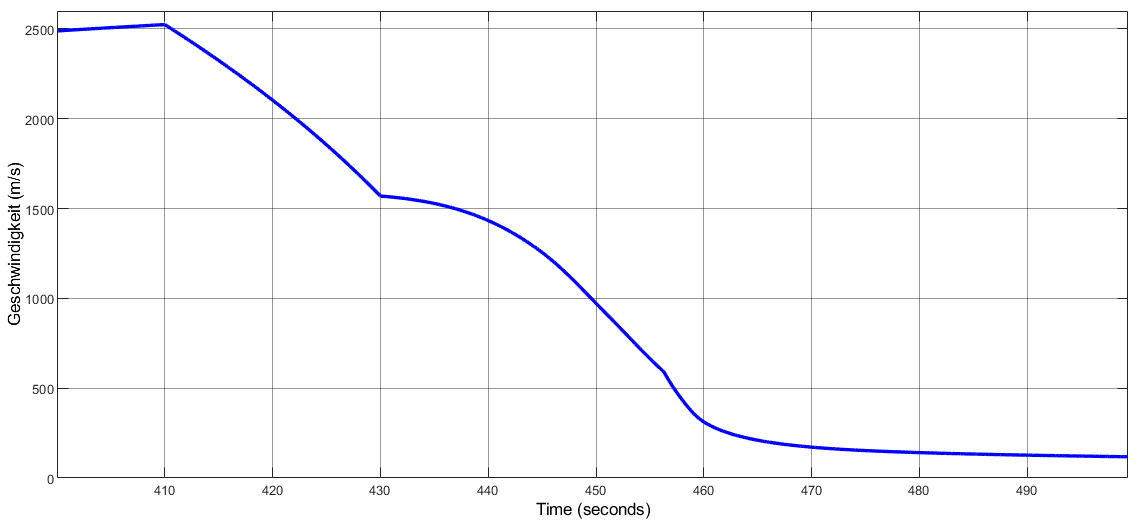
\includegraphics[width=0.9\textwidth]{vNormal.png}
	\caption{Fluggeschwindigkeit bei konstant gehaltener Neutralstellung}
	\label{abb_vNormal}
\end{figure}\\~\\
Dies war nun aber nur ein sehr simpler Missionsablauf, der den Grid Fins nicht viel abverlangt. Für die Auslegung müssen jedoch auch die worst-case-Szenarien berücksichtigt werden. Dazu zählt zum einem ein Ausschlag des Steuerwinkels, wodurch zum einem deutlich höhere Normalkräfte zu Stande kommen, aber auch die Axialkräfte deutlich ansteigen. Des Weiteren ist der Fall zu betrachten, dass der ReEntry-Burn ausfällt, beziehungsweise bewusst weggelassen wird, um die Wirtschaftlichkeit durch geringere Treibstoffmitnahme zu maximieren. In dem Fall würde die Raketenstufe mit deutlich höherer Geschwindigkeit in die Atmosphäre eintauchen, was zu enormen Belastungen führt.

Zu dem maximalen Lastfall kommt es, wenn kein ReEntry-Burn stattfindet und alle Grid Fins um $\eta = \pm 10^\circ$ ausgeschlagen sind. Die Finnen befinden sich dabei in x-Formation und der Ausschlag ist so ausgerichtet, dass ein Moment erzeugt wird, das den Nickwinkel erhöht. Die Kräfte, die in diesem Fall von den Grid Fins ausgehalten werden müssen sind für alle betragsmäßig gleich und in Abbildung \ref{abb_FExtreme} dargestellt. Während die Axialkraft nur leicht ansteigt, nehmen die Normalkräfte sehr hohe Werte an wie der Kraftvektor
\begin{equation}
	\vec{F}(t=440,7\mathrm{s})
	=\left(\begin{array}{c}817\mathrm{N}\\-6530\mathrm{N}\\-6183\mathrm{N}\end{array}\right)
\end{equation}
zeigt. Zu erkennen ist, dass der Wiedereintritt hochfrequenten Schwingungen ausgesetzt die Amplituden von bis zu $\Delta F_z = 3194$N besitzen. Wird nun aber davon ausgegangen, dass eine funktionstüchtige Reglung existiert, so kann diese Schwingung ausgeglichen werden und es käme ein Kraftvektor mit den Mittelwerten zu Stande.
\begin{equation}\label{eq_Fmax}
\vec{F}_\mathrm{geregelt}(t=440,7\mathrm{s})
=\left(\begin{array}{c}572\mathrm{N}\\-6415\mathrm{N}\\-4995\mathrm{N}\end{array}\right)
\end{equation}
Der Moment, in dem eine Machzahl von $Ma_\infty = 2$ erreicht qird und der Ballonschirm deployed, ist zwar in diesem Fall deutlich erkennbar, da die Raketenstufe in diesem Moment plötzlich herumgerissen wird, kann jedoch im Vergleich zu den Kräften bei "Max Q"\ vernachlässigt werden.
\begin{figure}[h] 
	\centering
	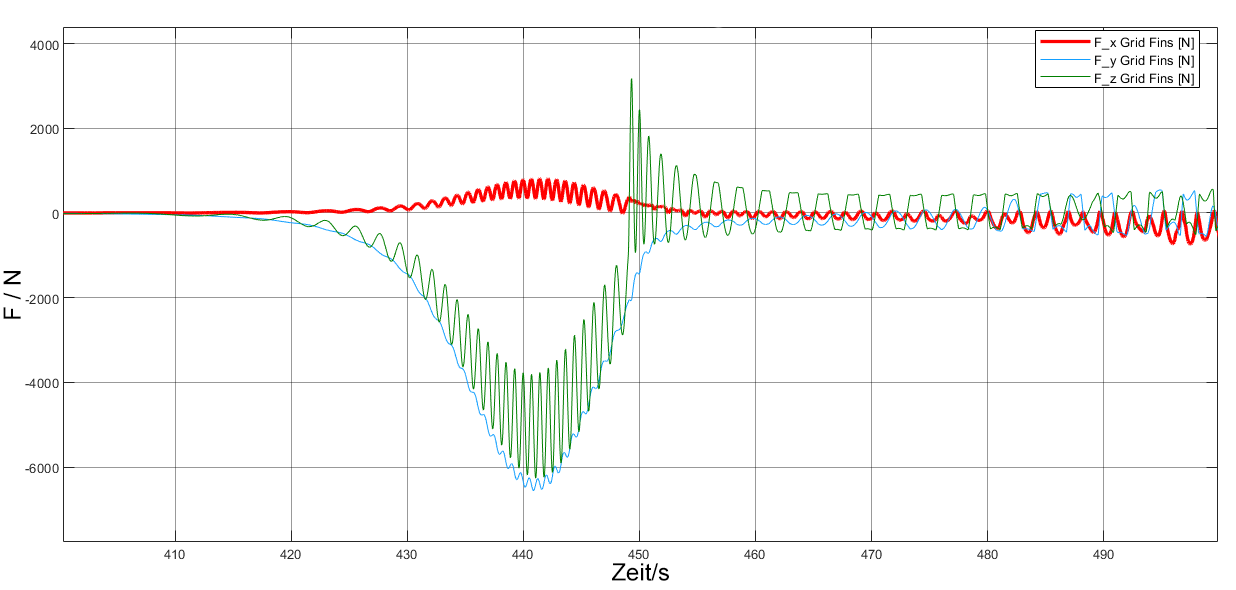
\includegraphics[width=0.9\textwidth]{F2Extreme4.png}
	\caption{Kräfte am Grid Fin beim maximalen Lastfall}
	\label{abb_FExtreme}
\end{figure}\\
\subsection{Geometrische Anforderungen}
Die Hauptmaße der Grid Fins sind hauptsächlich durch die Fertigung begrenzt. Ein Grid Fin soll also in einen entsprechenden 3D-Drucker mit den Maßen $300$x$300$x$400\mathrm{mm}^3$ passen. Für die Größe und Anordnung der Aktuatorik ist darauf zu achten, dass für alle vier Grid Fins jeweils zwei Motoren mit ihren zugehörigen Getrieben in den Raketendurchmesser von $1,1$m passen müssen. Das Innere dieses Durchmessers wird jedoch für die Bordelektronik benötigt, sodass sich die Aktuatorik am äußeren Rand befinden muss. Es ist des Weiteren eine Maximalhöhe von $0,15$m vorgesehen, die nicht überschritten werden darf.
\newpage
\section{Morphologischer Kasten}
Um eine Übersicht über die verschiedenen Designmöglichkeiten zu haben wird an dieser Stelle ein morphologischer Kasten, wie in er in Abbildung \ref{abb_MorphKastGF} zu sehen ist, eingeführt. Für fünf Designentscheidungen des Grid Fins sind dort unterschiedliche Teillösungen aufgelistet. Ganz links sind drei mögliche Zellformen gegeben. Es besteht die Wahl zwischen quadratischen, drei- und sechseckigen Geometrien. Hierbei sei aber wieder zu berücksichtigen, dass es auch zu einer Mischung mehrerer Formen kommen kann und besonders am Rand durch den Rahmen die Zellen ungleichmäßig verkleinert werden könnten.

Für die Form des gesamten Gitters stehen nur drei unterschiedliche Möglichkeiten zur Auswahl: Rechteck, Diamant oder auch eine dem Insektenflügel nachempfundene Struktur. Da jedoch die Maße noch nicht festgelegt sind kann die ersten der beiden Formen auch noch zum Quadrat werden. Des Weiteren kann es sein, dass die Geometrie an der einen Seite für die Anbringung noch angepasst wird.

Die größte Auswahl bietet sich bei den Wandquerschnittsformen. Rechteckig, abgerundet, beidseitig und einseitig spitzt, trapezförmig und dreieckig sind die sechs Optionen, die es hier gibt. Der Wandquerschnitt muss nicht überall die gleiche Form besitzen. So kann es kommen, dass das Gitter eine unterschiedliche erhält als der Rahmen. Die unteren beiden Formen sind zum Beispiel asymmetrisch, sodass sie nur für die Umrandung der Grid Fins in Frage kommen.

Als viertes wird die Fragestellung einer Krümmung gezeigt. Neben einem flachen Design kann der Grid Fin entweder zur Strömung hin konvex oder konkav gekrümmt sein. Dies ist abhängig davon in welche Richtung die Finne eingeklappt werden kann.

Im Grundlagenkapitel wurden drei verschiedene Arten der Pfeilung eines Grid Fins gezeigt. Da sie sich grundsätzlich unterschiedlich implementieren lassen, können sie theoretisch sogar in Kombination gewählt werden. Der Pfeilungswinkel ist für die Varianten noch frei wählbar und auch negative Winkel, also Vorwärtspfeilung, ist denkbar. Für die lokale Pfeilung der Zellen rückt der Unterschied zwischen Vorwärts- und Rückwärtspfeilung durch die Unterscheidung vom Berg- und Tal-Typus noch mehr in den Vordergrund. Wichtig ist noch anzumerken, dass die konfigurelle Pfeilung keinen direkten Einfluss auf das Design der Grid Fins an sich hat, sondern sich durch den Bewegungsspielraum der Aktuatorik umsetzten lässt.
\begin{figure}[h]
	\centering
	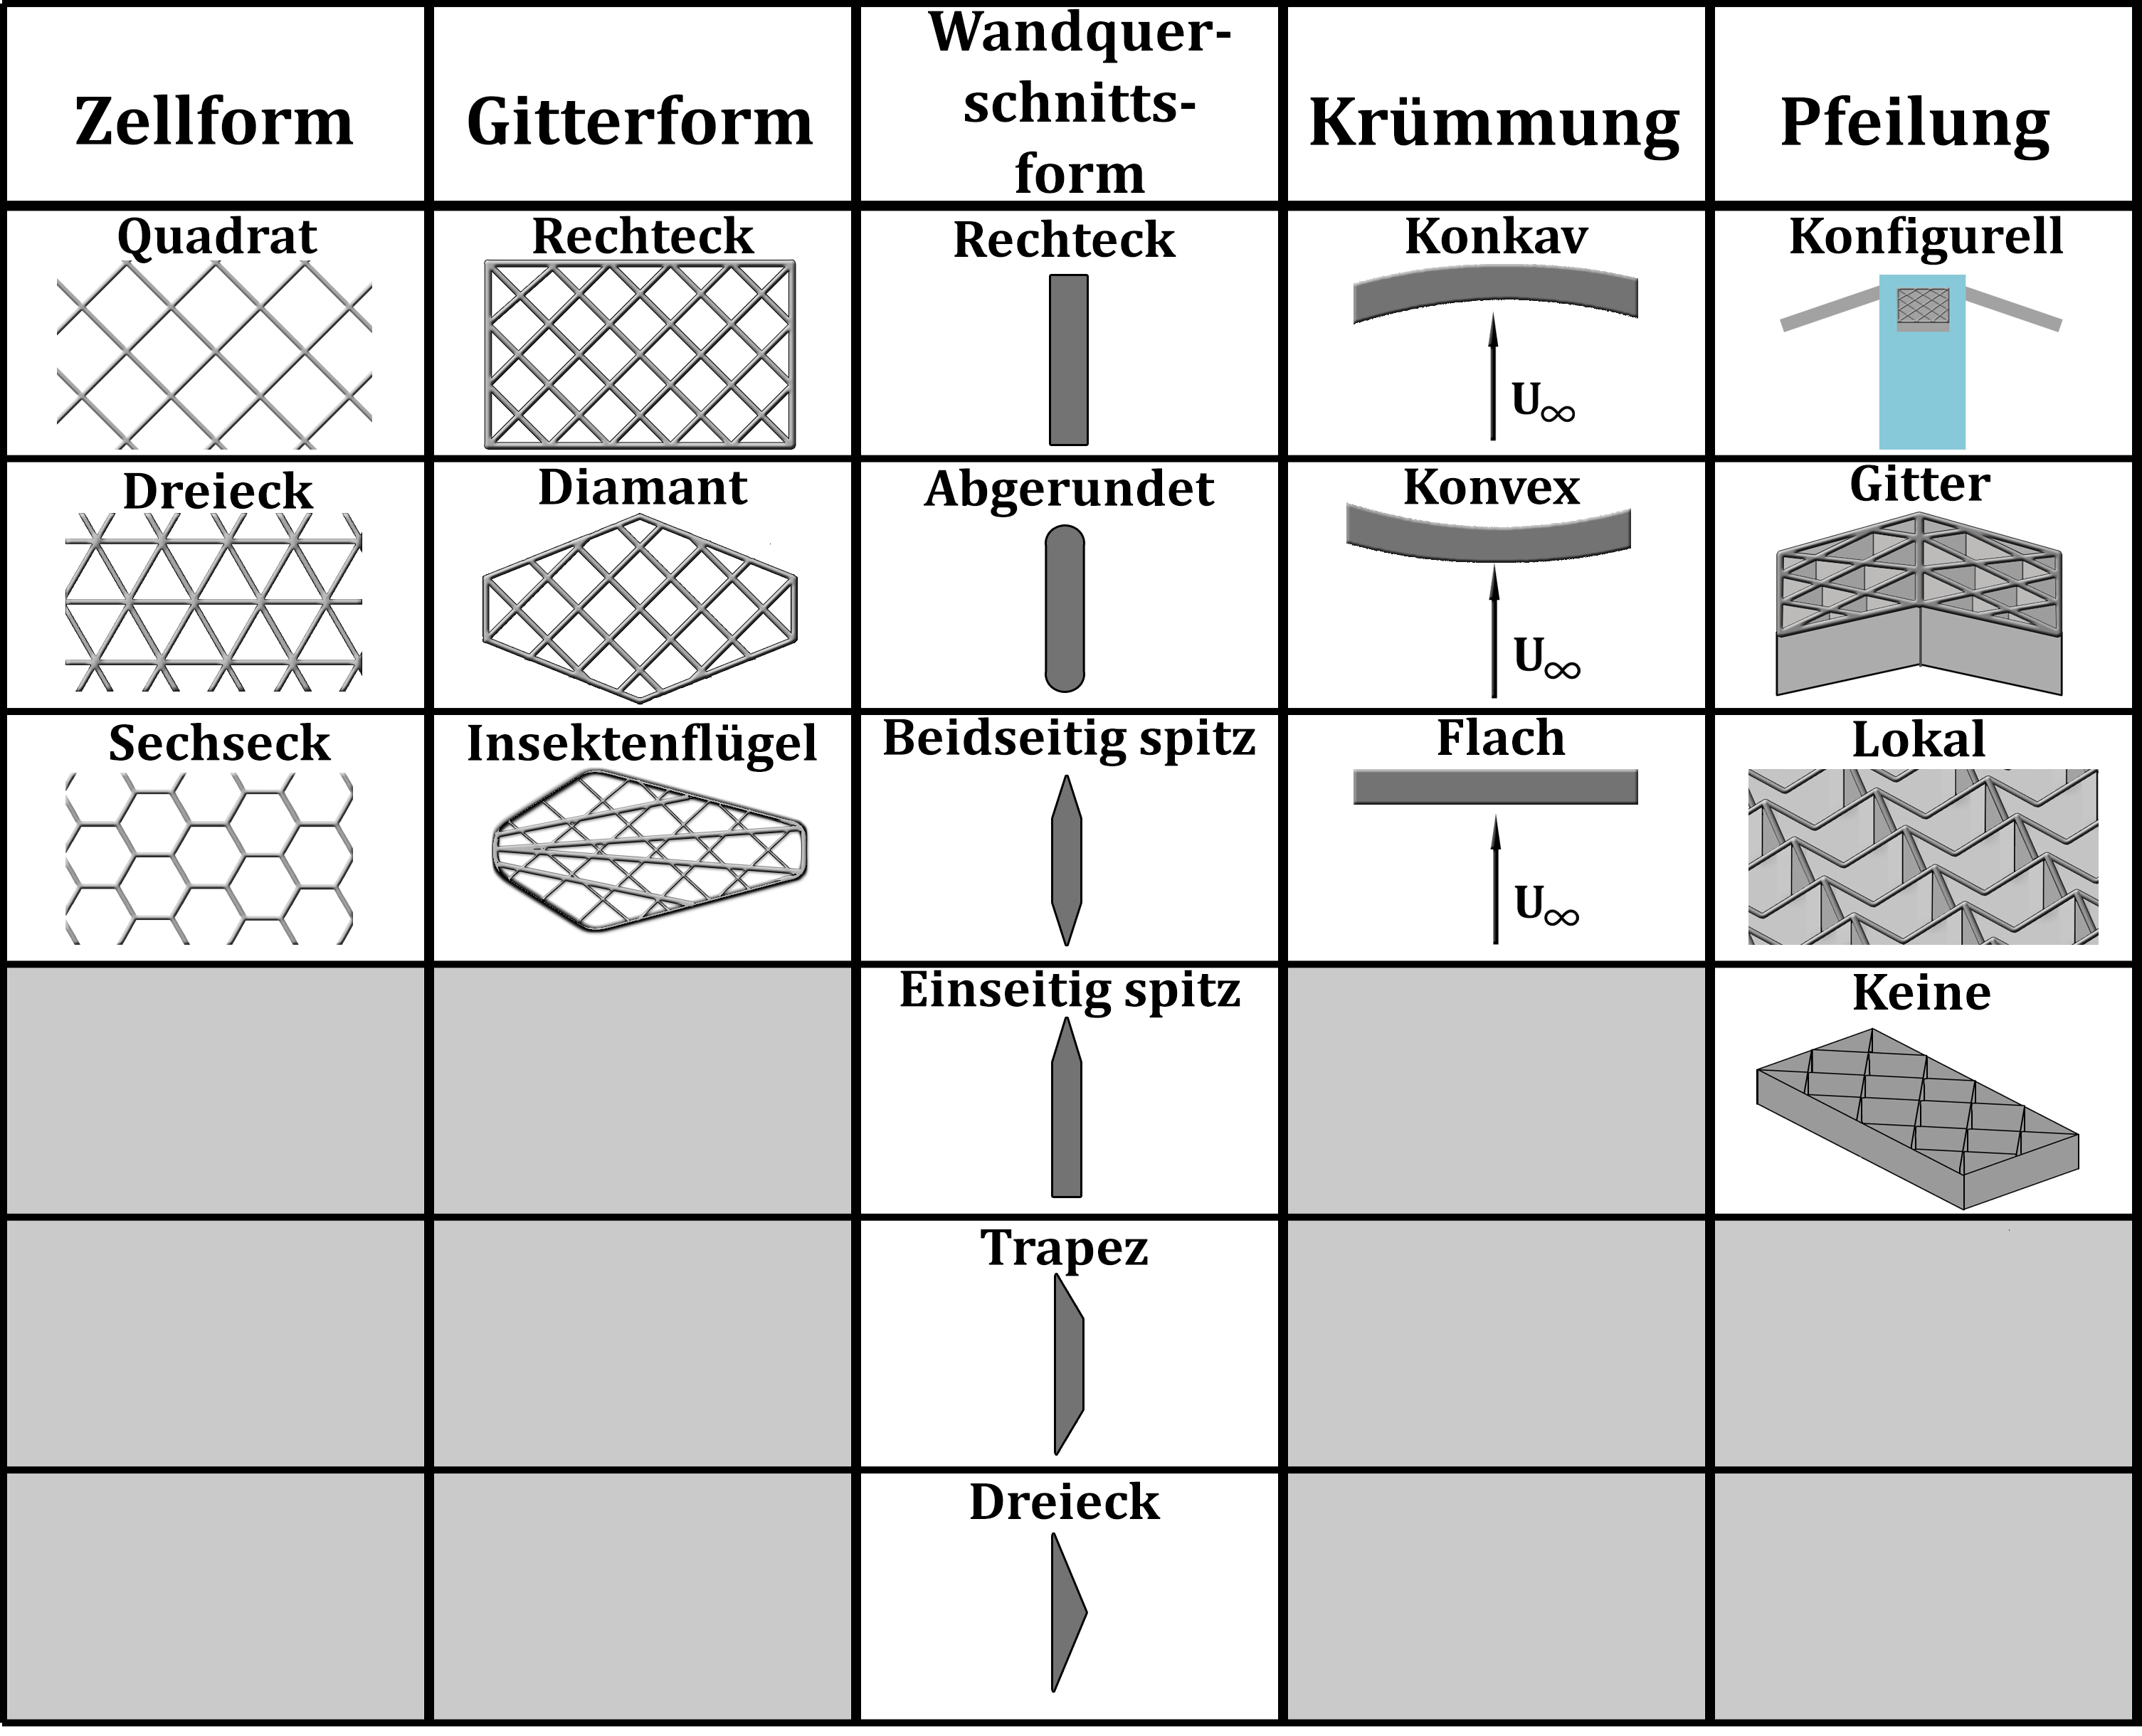
\includegraphics[width=0.9\textwidth]{Morphologischer Kasten GF V2.png}
	\caption{Morphologischer Kasten für die Grid Fins}
	\label{abb_MorphKastGF}
\end{figure}\\~\\
Für den Entwurf der Aktuatorik wurde ein zweiter morphologischer Kasten erstellt. Dieser ist in Abbildung \ref{abb_MorphKastAk} zu sehen und zeigt drei verschieden Designkategorien. Da die Grid Fins zwei unabhängige Freiheitsgrade haben, können für den Steuer- und Klappwinkel separat unterschiedliche Lösungen aus dem morphologischen Kasten gewählt werden.

Eine wichtige Designentscheidung ist der Aktuator, da er bestimmt was als Energiequelle genutzt wird und hat somit einen großen Einfluss auf Gewicht und Kosten. Eine Möglichkeit ist die elektrische Energie zu nutzen und diese mit einem Elektromotor direkt die mechanische Arbeit verrichten zu lassen. Hierbei muss noch die Wahl getroffen werden, ob linear oder rotatorischer Motor vorgezogen werden soll. Alternativ kann auch ein hydraulisches oder gar pneumatisches System verwendet werden. Da Grid Fins zwei Freiheitsgrade haben, können diese über unterschiedliche Aktuatoren, die auch unterschiedlicher Art sein können, bewegt werden. Also muss in diesem Punkt für beide Rotationen einzeln entschieden werden.

Über ein Getriebe wird die Leistung des Aktuators auf die Grid Fins übertragen, um mehr Spielraum für Kraft, Moment, Drehzahl und Orientierung des Aktuators zu gewährleisten. Eine Möglichkeit bietet das klassische Zahnradgetriebe. Viele Paarungen wie Stirn-, Kegel-, Schrauben- oder Schneckenräder sind denkbar. Kräfte und die zugehörige Bewegungsgeschwindigkeit lassen sich auch durch hydrostatische Getriebe beeinflussen. Momente und Drehzahlen können durch hydrodynamische Getriebe verändert werden. Generell sind durch Kombinationen beliebig komplexe Systeme möglich.

Als letztes beschäftigt sich der Morphologische Kasten in Abbildung \ref{abb_MorphKastAk} mit der Lagerung. Hierbei wird generell zwischen den Wälz- und Gleitlagern unterschieden. Beide bieten jedoch noch mehr Entscheidungsfreiheiten. So gibt es einige unterschiedliche Wälzkörper, wie Kugeln, Zylinder, Kegel oder Pendelrollen. Auch Gleitlagern können weiter zu statischen und dynamischen unterteilt werden, je nach Art der Schmierfilmdruckerzeugung.
\begin{figure}[h]
	\centering
	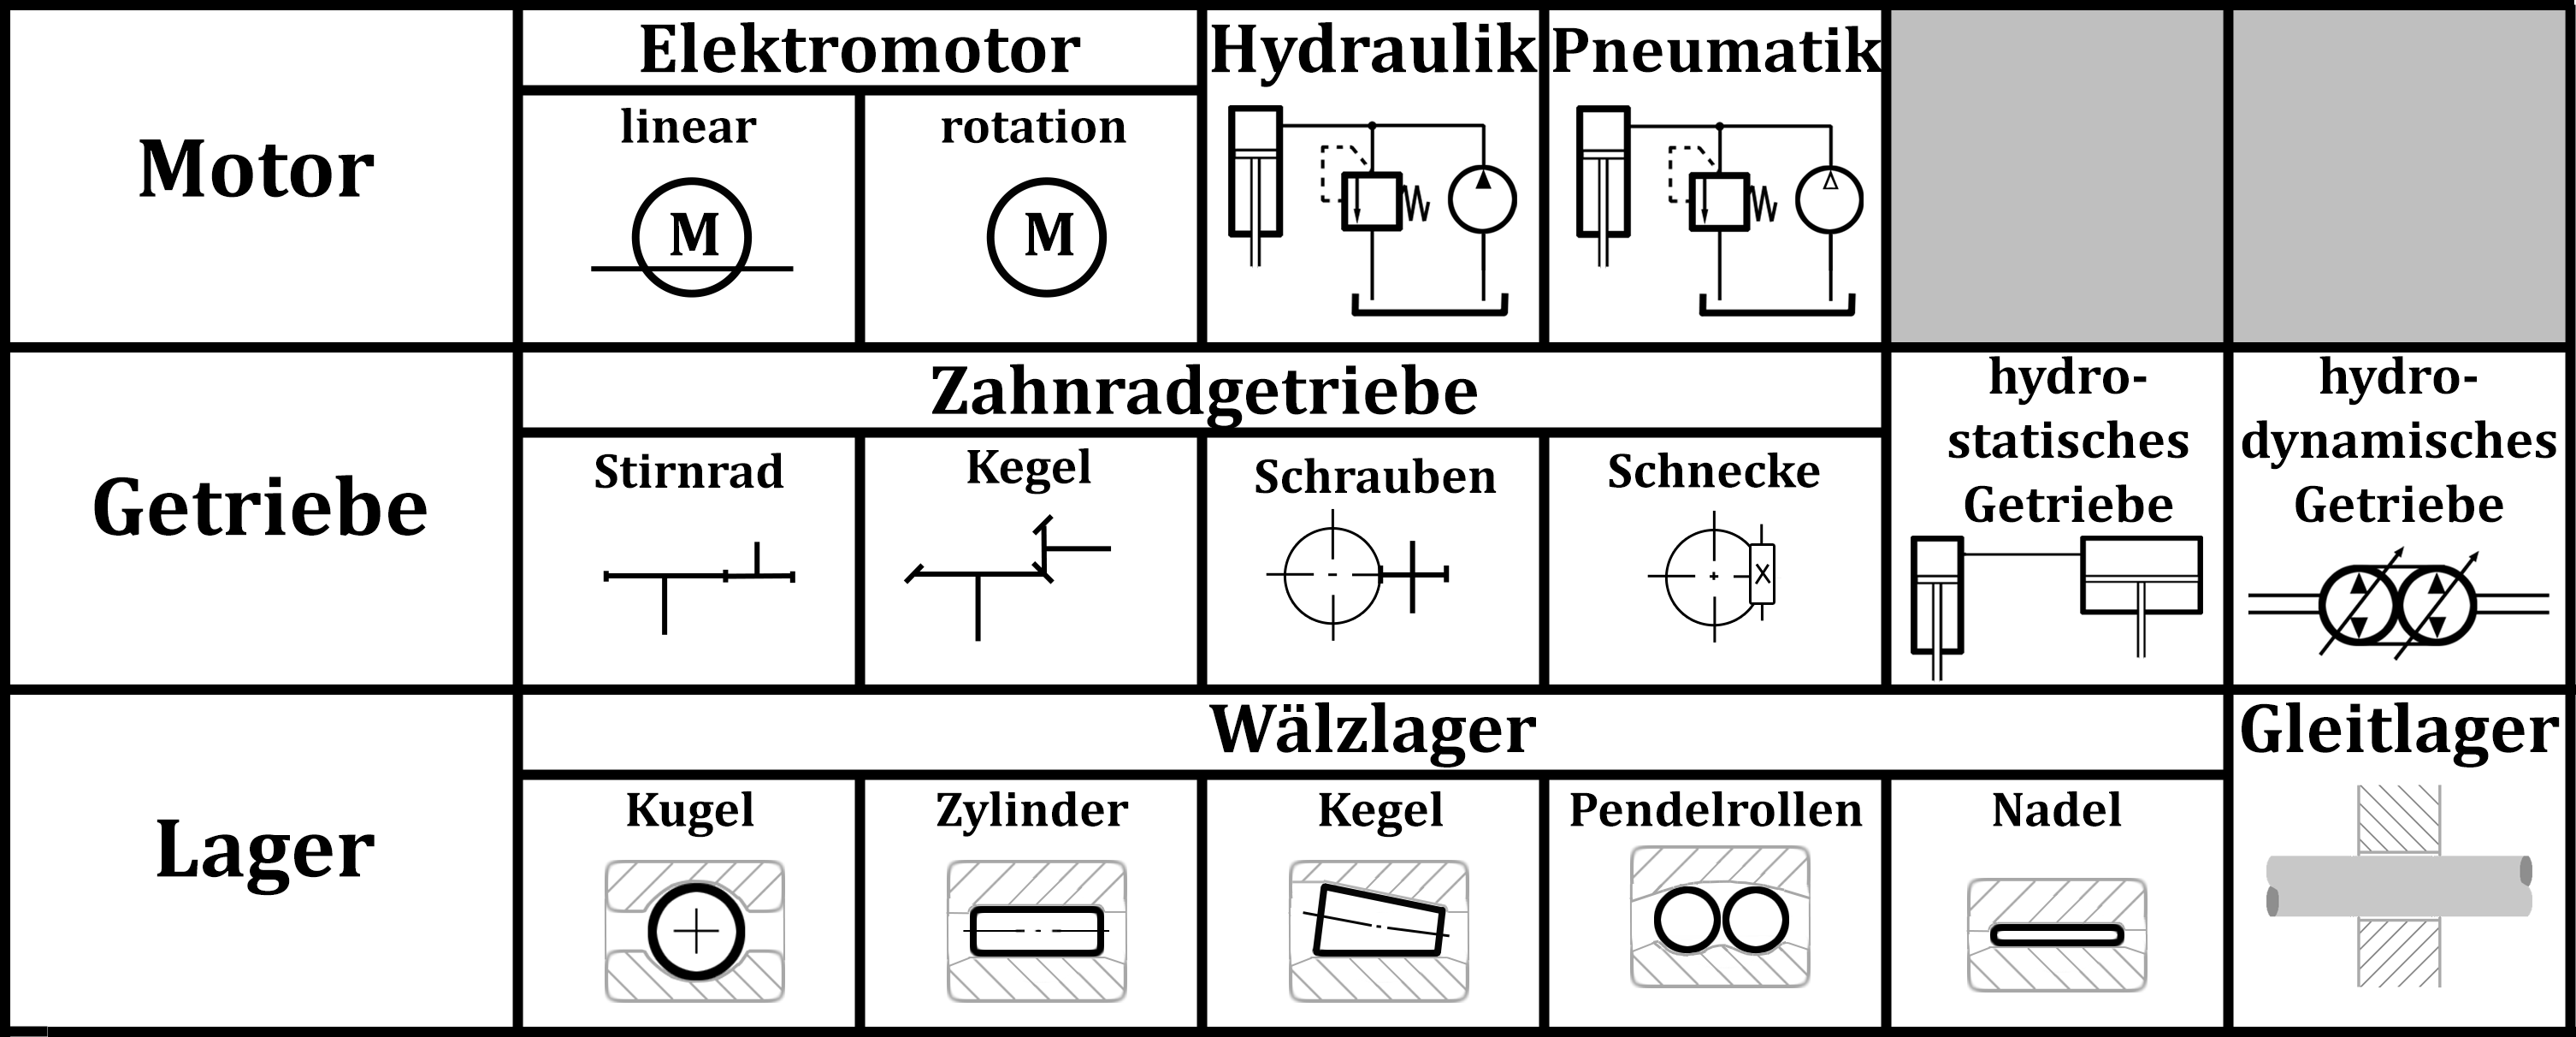
\includegraphics[width=\textwidth]{Morphologischer Kasten Ak.png}
	\caption{Morphologischer Kasten für die Grid Fin Aktuatorik}
	\label{abb_MorphKastAk}
\end{figure}\\
Es gibt jedoch noch weitere Designentscheidungen, die sich nicht in einem morphologischen Kasten pragmatisch darstellen lassen. So müssen zum einen noch die Dimensionen des Moduls und Lage der Aktuatoren in der Rakete definiert werden. Zum anderen stellt sich die Frage welche Zellgröße $g$ und Wandstärke $d$ an welcher Stelle gewählt wird. Es besteht auch noch die Möglichkeit die Grid Fins mit zusätzlichen Features auszustatten. Eine Option wären hier zusätzliche Stützstreben oder sogar durch die additive Fertigung ermöglichte, in das Material integrierte Strukturen, wie zum Beispiel Kühlkanäle oder Drucksensoren.
\newpage
\section{Komponentenrecherche und -auswahl}
Als nächstes werden nun die Ergebnisse der Komponentenrecherche beschrieben und auf Grund der Systemanforderungen mit Hilfe der morphologischen Kästen eine vorläufige Wahl getroffen.
\subsection{Materialwahl}
Es stehen vier verschiedene Werkstoffe zur Auswahl, die sowohl für die Raumfahrt, als auch additive Fertigung in Frage kommen: Edelstahl, Inconel (eine Nickellegierung), Aluminium- und Titanlegierungen. Tabelle \ref{tab_Werkstoffe} im Anhang zeigt Vertreter dieser Werkstoffgruppen, wie sie vom 3D-Druck-Anbieter EOS benutzt werden, und vergleicht ihre Eigenschaften. Die vielversprechendsten Vertreter der jeweiligen Werkstoffgruppen, oder jede zu denen genügend Daten vorliegen, sind zusätzlich der Übersicht halber ein weiteres Mal in Tabelle \ref{tab_WerkstoffeKlein} dargestellt.
\\~\\
Eine wichtige Eigenschaft ist natürlich die Dichte $\rho$. Hier liegen die Aluminiumlegierungen ganz klar vorne mit nur $2,57$g/cm$^3$, aber auch Titan bietet vergleichsweise gute Werte. Die Edelstähle und Nickellegierungen hingegen sind deutlich schwerer, was wiederum zu einer geringeren Wirtschaftlichkeit der Rakete führen würde, da die Masse stattdessen als Nutzlast genutzt werden könnte. Die Dichte alleine ist jedoch nicht sehr aussagekräftig, da bei geringerer Festigkeit auch dickere Strukturen benötigt werden. So zeigt Tabelle \ref{tab_Werkstoffe} zusätzlich die Streckgrenze $R_{p,0.2}$. Pro Werkstoff sind hier zwei Werte angegeben, da durch die additive Fertigung die Homogenität verloren geht, sodass die Festigkeit in den Schichten höher ist als senkrecht zu ihnen. Nur der hier ausgewählte Edelstahl hat vernachlässigbare Inhomogenitäten. Die Werte sind in Tabelle \ref{tab_WerkstoffeKlein} für alle Werkstück direkt nach der Fertigung außer beim Inconel. Mit einer thermischen Nachbearbeitung können die Streckgrenzen noch etwas erhöht und die Inhomogenitäten abgeschwächt werden. Es zeigt sich, dass die Festigkeiten der Materialien weit auseinander gehen. So kann zum Beispiel Aluminium fast nur 20\% der maximal Belastung von Titan aushalten. Um nun die beiden Aspekte der Dichte und Streckgrenze miteinander zu verbinden wird die spezifische Festigkeit $R_\mathrm{spez.}=\frac{R_{p,0.2}}{\rho}$ , also die Streckgrenze im Bezug auf die Masse, eingeführt. Es wurde der untere Wert der Streckgrenze verwendet und wenn verfügbar ohne Wärmebehandlung. Hier hebt sich Titan mit $R_\mathrm{spez.}=254$Nm/g klar von den anderen ab, während Aluminium trotz der geringen Dichte von den anderen Werkstoffgruppen großteils übertroffen wird. Hier sei auch anzumerken, dass der Vorsprung von Inconel über den Edelstählen auf die Verwendung der Materialwerte bei Wärmebehandlung zurück zu führen sind. Rechne man die spezifische Festigkeit des in diesem Kapitel dargestellten Stahls 1.4542, so erhält man einen noch besseren Wert von $R_\mathrm{spez.} = 162,0$Nm/g. Die Materialwerte von Titan scheinen sich zwar nicht groß durch eine Wärmebehandlung zu ändern, jedoch ist der Werkstoff in dieser Bewertungskategorie dank der geringen Dichte noch immer deutlich überlegen.
\\~\\
Auch wenn die Maximierung der spezifischen Festigkeit und somit eine Minimierung der Masse eine Senkung der Kosten zur Folge hat, ist der Materialpreis nicht zu vernachlässigen. Es lässt sich zwar kein genauer kg-Preis festlegen, da die entstehenden Kosten am Ende von der genauen Geometrie des Bauteils abhängen, dennoch kann eine qualitative Einordnung der verschiedenen Materialien vorgenommen werden. Hierzu wurden von der Rapidobject GmbH für die Fertigung eines Grid Fins Modells ($V \approx 100\mathrm{mm}^3$) mit verschiedenen Materialien erstellt. Dieses Modell ist etwas kleiner, als das spätere Endprodukt und auch die Geometrie steht noch nicht fest. Es zeigt dennoch gut die preislichen Unterschiede der Werkstoffe.
SO hat zum Beispiel Aluminium mit nur $1.508,9$€ die mit Abstand geringsten Kosten, während Titan das doppelte kostet. Der Edelstahl und Inconel liegen beide eng aneinander dazwischen.
\\~\\
Nicht zur die mechanische Belastbarkeit der Materialien ist entscheidend, sondern natürlich auch die thermische, um die extremen Temperaturen des Wiedereintritts zu überstehen. Hierfür muss ein Blick auf die maximale Einsatztemperatur $T_\mathrm{E, max}$ geworfen werden. Dies ist die Temperatur, bei der die mechanischen Eigenschaften des Werkstoffs stark abnehmen, sodass nicht mehr sein volles Potenzial genutzt werden kann. Aus Mangel an Daten wurde jedoch für Titan hier die Temperatur, bei der Warmumformung stattfindet, verwendet. Bei dieser Temperatur sind die Metalle weich genug, um sie verarbeiten zu können. Die wahre maximale Einsatztemperatur sollte also etwas niedriger liegen. Diese darf jedoch nur nicht langfristig überschritten werden, sodass bei der kurzen Wiedereintrittsphase auch höher Temperaturen auftreten können, ohne zum Versagen zu führen. Ein Blick auf andere Raketen, wie zum Beispiel die Flacon 9, zeigt, dass Grid Fins aus Titan und Edelstahl in diesem Fall den Bedingungen standhalten während es bei Aluminium Grid Fins zum Verlust der Form kam. Um also eine bessere Vergleichbarkeit zu erreichen, wurde zusätzlich auch noch die Schmelztemperatur aufgelistet.
\begin{table}[h] 
	\centering 
	\begin{tabular}{c|c|c|c|c|c|c|c} 
		Werkstoff&Bezeichnung&$\rho$/$\frac{k\mathrm{g}}{\mathrm{cm}^3}$&$R_{p,0.2}$/MPa&$R_\mathrm{spez.}$/Nm/g&Preis/€&$T_\mathrm{E, max}$/$^\circ$C&$T_\mathrm{Schmelz}$/$^\circ$C\\ 
		\hline 
		Aluminium&AlSi10Mg&2,57&230-270&89,5&1.508,93&530&557\\ 
		Edelstahl&1.4542&7,79&861-861&110,5&2.559,27&550&1400\\ 
		Inconel&IN 718&8,15&1140-1245&140,5&2.597,71&700&1260\\ 
		Titan&TiAl6V4&4,41&1120-1140&254,0&3.085,12&>700&1630\\ 
	\end{tabular} 
	\begin{flushright} 
		\flushbottom{Quellen: \cite{eos, preise, T1.1, T1.4, T2.1, T2.4, T2.3, T3.5, T3.8}} 
	\end{flushright} 
	\caption{Vergleichsdaten der unterschiedlichen Werkstoffe (Auswahl)}
	\label{tab_WerkstoffeKlein}
\end{table} \\
Aluminiumlegierungen zeigen bei der thermischen Belastbarkeit sehr große Schwäche, was sie für diese Anwendung zu ungünstigen Kandidaten macht. Die Titanlegierungen hingegen haben zwar mit einer extrem hohen spezifischen Festigkeit $R_\mathrm{spez.}$ ein exzellentes Leichtbaupotenzial und auch ihre ertragbaren Temperatur sind unschlagbar, sodass sie eigentlich ideale Kandidaten als Werkstoff für Grid Fins sind. Titan hat jedoch einen enormen Nachteil, was den Preis betrifft. Für einen kleinen Microlaucher, der sich gegenüber vielen Konkurrenten durchsetzten muss, ist Preis ein sehr großer Faktor der Titan als Material disqualifiziert. Edelstahl und Inconel hingegen überzeugen mit ähnlichen Werten, so ist der Preis für diese beiden Werkstoffe beinahe identisch. Wir für beide Materialien der wärmebehandelte Zustand betrachtet, hat der Edelstahl 1.4542 zwar einen höheren Wert, die maximale Einsatztemperatur $T_\mathrm{E, max}$ ist nach Angaben der Rapidobject GmbH für Inconel 718 höher \cite{preise}. Da jedoch die Schmelztemperaturen auf ähnlich hohem Niveau liegen und Anwendungsbeispiele wie die Grid Fins der Falcon 9 zeigen, dass die Einsatztemperatur von Edelstahl hoch genug liegt, sind die $\Delta R_\mathrm{spez.} = 21,5$Nm/g ein wichtigere Vorteil. Die Grid Fins werden folglich aus \textbf{Edelstahl 1.4542} hergestellt.
\subsection{Gitterdesign}
Für den Design des Gitters wird eine Auswahl der einzelnen Komponenten aus dem morphologische Kasten in Abbildung \ref{abb_MorphKastGF} getroffen.
\\~\\
Als erster Punkt werden dort verschiedene Zellformen dargestellt. Wie im Grundlagenkapitel in Abschnitt \ref{sec_zellform} dargelegt, hat die Zellform so gut wie keinen Einfluss auf die Aerodynamik. Nur im Transschall erzeugt die Wabenstruktur weniger Normalkraft. Dies kann jedoch vernachlässigt werden, da nur Machzahlen $Ma_\infty >2$ relevant ist, weil unterhalb der Ballute auslöst und die Grid Fins nicht mehr relevant sind. Bei traditionellen Fertigungsverfahren ist es in den meisten Fällen einfacher und somit günstiger die Struktur aus geraden Elementen zu fertigen. Bei der additiven Herstellung ist dieser Aspekt jedoch irrelevant, sodass nur die strukturmechanischen Eigenschaften der Zellform relevant sind. Da in den meisten Fällen \textbf{viereckige Zellen} mit maximal \textbf{dreieckigen Seitenelementen} benutzt wurden, wird auch diese praxiserprobte Variante gewählt. Zudem gibt es hierzu die meisten Daten, was die Wahrscheinlichkeit von unerwartetem Verhalten minimiert.
\\~\\
Auch für die Gitterform gibt es unterschiedliche Möglichkeiten. Da jedoch keine Studien über ihren Einfluss auf die erzeugbaren Kräfte existieren, muss auch hier in anderer Hinsicht argumentiert werden. Um den rechteckigen Baumraum eines 3D-Drucker ideal nutzen zu, bietet sich auch eine rechteckige Gitterform an. Dies ermöglicht eventuelle einen kleineren Drucker zu nutzen und somit Fertigungskosten einzusparen. Auch auf diese Form lässt sich die Zuspitzung des Grid Fins, wie sie bei den anderen beiden Varianten zu sehen ist anwenden, um einen besseren Kraftfluss zu ermöglichen. Zusätzlich lassen sich durch additive Fertigung die Außenkanten ohne großen Mehraufwand wie beim Insektenflügel abrunden, was die Struktur weiter entlasten sollte. Somit ist die Wahl auf ein \textbf{Rechteckgitter} mit \textbf{Zuspitzung zur Einspannung} hin und \textbf{abgerundeten Außenkanten }gefallen.
\\~\\
Die Wandquerschnittsform hat im Gegensatz zu den anderen beiden bisherigen Aspekten einen großen Einfluss auf die Aerodynamik oder genauer gesagt den Widerstand. Dieser Effekt wurde im Grundlagenkapitel in Abschnitt \ref{sec_wandquerschnitt} behandelt. Auch wenn Widerstand nicht zwangsläufig negativ zu bewerten ist, da die Rakete so beim Wiedereintritt stärker abgebremst wird, bedeutet mehr Widerstand auch mehr Belastung, also kürzere Lebensdauer beziehungsweise schwererer Grid Fin. Der Mehraufwand von komplexeren Querschnittsformen fällt durch die additive Fertigung auch weg. So wird für das \textbf{Gitter} eine \textbf{beidseitig spitze} Form gewählt, wegen des geringeren Widerstandes. Für den \textbf{Rahmen} wird die \textbf{Trapezform} verwendet, da die Außenkante flach sein kann. Es wurde sich gegen die Dreiecksform entschieden, obwohl die den geringsten Widerstand liefert, da weniger Material außen ist und somit schlechter Biegemomente um eine horizontale Achse aufgenommen werden können. Des Weiteren ist der Effekt auf die Normalkraft, wenn nur angeschrägte Flachen existieren unbekannt.
\\~\\
Auch die Krümmung hat wieder eine vernachlässigbar kleinen Einfluss auf die Aerodynamik von Grid Fins. Durch die additive Fertigung im 3D-Drucker ist auch kein wirklicher zusätzlicher Aufwand damit verbunden. Um beim Wiedereintritt den Grid Fin nicht gegen die Widerstandskraft halten zu müssen, soll er zum Triebwerk hin angelegt werden. Somit wird der Grid Fin mit einer zur Anströmung \textbf{konkaven Krümmung} modelliert.
\\~\\
Mit einer Pfeilung lässt sich nun wiederum die wirkenden Axialkräfte verändern. Mit der konfigurellen Pfeilung lassen sich diese Kräfte um bis zu das 4-fache erhöhe. Dies würde zu einer deutlich stärkeren Belastung führen, wodurch der Grid Fin stabiler und somit schwerer und unwirtschaftlicher wird. Sollte nun hingegen eine verstellbare konfigurelle Pfeilung implementiert werden, so steigen die Anforderungen an den Aktuator wieder deutlich an. Dies würde zu einer deutlichen Kostensteigerung führen ohne signifikante Vorteile, da der restliche Körper noch immer deutlich größere Anteile zum aerodynamischen Widerstand liefert. Somit wir eine Pfeilung der Konfiguration an dieser Stelle ausgeschlossen.

Die Pfeilung des Gitters ist wiederum nicht mit der Krümmung verträglich. Das bessere Anlegen des Grid Fins an die Außenhülle der Rakete ist an dieser Stelle der Widerstandsreduzierung einer solchen Pfeilung vorzuziehen.

Bleibt nun also nur noch die lokale Pfeilung, welche keinen Einfluss auf andere Designparameter hat. Auf der Außenseite, beziehungsweise der Stromabwärtsseite, kommt sie jedoch auch nicht in Frage, da sie im eingeklappten Zustand beim Raketenstart in die Strömung ragt und somit zusätzlichen Widerstand verursachen würde. Auf der \textbf{luv-Seite} hingegen ist die \textbf{lokale Pfeilung} eine gute Möglichkeit der Widerstandsreduzierung und wird deswegen implementiert. Die wohl bekannteste Verwendung der lokalen Pfeilung befindet sich an den Grid Fins der Falcon 9, welche den Berg-Typus verwendet. Die Analysen von Guyot und Schülein \cite{PeakValley}, dass, auch wenn beide Varianten den gleichen Widerstandsvorteil habe, die Normalkraft, bei dem Tal-Typus jedoch höher ist. Da die Grid Fins von SpaceX aber auch keine spitze Vorderkante haben, würden bei ihnen eine lokale Pfeilung des Tal-Typus an den Schnittstellen nahezu zu einer Sackgasse für die Strömung kommen, was einen großen Widerstand bewirkt. Da bei diesem Grid Fin die Gitterwände eine doppel-spitzen Wandquerschnitt haben, wie es auch bei den Untersuchungen von Guyot und Schülein der Fall war, wird hier der \textbf{Tal-Typus} verwendet. Da das größte Bedenken hier die Stabilität der Zacken betrifft, die sich im Gegenteil zum Berg-Typus nicht gegenseitig stützen, kann es sein, dass nach der FEM-Anaylse der Typus noch gewechselt wird.
\subsection{Peripherie und Aktuator}
Für alle der drei Energiemedien ist sind schon Vertreter in der Rakete installiert, die unter Umständen genutzt werden könnten. Da sich die Grid Fin Aktuatorik im selben Abschnitt wie die Boardelektronik der ersten Stufe befindet, sind auch hier direkt die Batterien, mit denen Elektromotoren betrieben werden können. So wird mit ihnen zum Beispiel auch die elektrischen Treibstoffpumpen für die Triebwerke mit Strom versorgt. Somit liegt direkt auch schon ein Hochdruckfluid vor, welches als Druckmittel für die Hydraulik genutzt werden könnte. Da sich dieses jedoch am anderen Ende der Rakete befindet und dafür sowohl ein Eingriff in die komplexen Triebwerke, so wie eine Abhängigkeit von vorhandenem Treibstoff oder LOX zu Stande kommt, ist dies eine weniger plausible Möglichkeit. Sodass eine eigene elektrische Pumpe und Druckmittel eine realistischere Umsetzung für eine Hydraulik wären. Für eine Pneumatik könnte jedoch ein vorhandenes System genutzt werden. Der Heliumtank für den Druckausgleich in den Tanks liegt direkt unterhalb der Elektronik und es existieren sogar schon Leitungen, die das Gas in diesen Bereich der Rakete für das RCS transportieren.
\\~\\
Da sowohl für den Klappwinkel, als auch den Steuerwinkel unterschiedliche Anforderungen existieren, die auch andere Lösungsmöglichkeiten zulassen, werden diese im Folgenden getrennt betrachtet.
\subsubsection{Klappwinkel}
\subsubsection{Steuerwinkel}
\subsection{Getriebe und Lagerung}

\section{Festlegung des Modelldesigns}\label{sec:modelldesign}
Nun da das Design feststeht, muss nur noch die Größe der einzelnen Parameter festgelegt werden. Die Größe der Querschnittsfläche $A$ ist abhängig von der Auftriebserzeugung, die gewährleistet werden soll. Aus der Simulation ist bekannt, dass ungefähr
\begin{equation}
	A \cdot C_{N\alpha}= 0,00432 \mathrm{m}^2/^\circ
\end{equation}
bei einer Machzahl von $Ma_\infty = 2.0$ und $\alpha = 0^\circ$ gelten soll. Da die einzelnen Modellierungsparameter hauptsächlich einen Einfluss auf den Widerstand haben und die Normalkraft, wir von einem ähnlichen Wert von $C_{N\alpha}$ ausgegangen, sodass auch eine Fläche von $A=0,9\mathrm{m}^2$ benötigt wird.

Das Verhältnis von Zellgröße zur Sehnenlänge kann jedoch den Auftriebsbeiwert verändern. Da aber nur Studien zum niedrigen Unterschall, bei denen ein Maximum bei gleicher Länge dieser beiden Parameter erreicht wird, wird hier ein Blick auf die bisher verwendeten Grid Fins geworfen. Wie Abbildung \ref{abb_f9_GF} zu erkenn gibt verwendet SpaceX bei seiner Falcon 9 auch ein Verhältnis von ungefähr 1:1, während Chinas Chang'e eine etwas kleinere Zellgröße zu besitzen scheint (vgl. Abbildung \ref{abb_change}). Da jedoch die Grid Fins in den meisten Studien die gleiche Zellgröße wie Sehnenlänge haben, lässt dies vermuten, dass die auch im Überschall dadurch die höchsten Normalkraftwerte erzeugt werden. Also wird auch hier dieses Verhältnis verwendet und der Wert $C_{N\alpha}$ und somit auch die Fläche müssen nicht verändert werden. Nun wird aus gängigen Werten für die Sehen ein Wert für diese festgelegt, sodass die zwei Parameter mit $\mathbf{s=g=0,04m}$ festgelegt werden.

Bei der Höhe $h$ und Breite $b$ können nun Werte gewählt werden, die ganzzahlig durch die Diagonale in der Zelle teilbar ist. Wird nun ein Seitenverhältnis von 5:6 gewählt, was zu einer Höhe von $\mathbf{h= }6\cdot g\sqrt{2}=\mathbf{339,4mm}$ und einer von $\mathbf{b= }5\cdot g\sqrt{2}=\mathbf{282,8mm}$ führt. Dies muss auch in den Bauraum eines Druckers passen. Dieser hat zwar nur eine Grundfläche von 300x300mm$^2$, aber da er 400mm hoch ist kann dich Diagonale von 500mm genutzt werden, indem in diese Eben auch die Höhe des Grid Fins gelegt wird. Die Fläche die durch die Höche und Breite des Grid Fins aufgespannt wird liegt mit $0,096\mathrm{m}^2$ noch etwas über der angestrebten Fläche. Jedoch muss diese noch um die vier halbe Zellen reduziert werden, da sich die Geometrie zur Einspannung hin schmälern soll. Übrig bleibt eine Fläche von $A=h\cdot b-2g^2=0,0928\mathrm{m}^2$.

Da sich an der Wanddicke $d$ im Laufe der FEM-Simulationen vermutlich am meisten ändern wird, soll an dieser Stelle nur ein kurze Überschlagsrechnung gemacht werden. Angenommen wird, dass die Wandstärke nicht in der Gitterform über die Breite verteilt ist, sondern alle zusammen addiert einen Balken mit der Gesamtdicke $d_\mathrm{ges.}(x_h)$ bilden. $x_h$ ist hierbei eine Koordinate die sich über den Grid Fin in Höhenrichtung spannt mit $x \epsilon [0, h]$. Dieser wird nur durch die maximale Kraft in Sehnenrichtung gleichmäßig auf der gesamten Länge $h$ und Breite $d_\mathrm{ges}(x_h)$ belastet. Die Kraft in Sehnenrichtung $F_s$ wird aus dem maximalen Kraftvektor in Gleichung \ref{eq_Fmax} bestimmt. Dieser ist im körperfesten Koordinatensystem gegeben, sodass er bei einem Steuerwinkel von $\delta = 10^\circ$ und in x-Konfiguration $\lambda=45^\circ$ noch wie folgt umgerechnet werden muss.
\begin{equation}
	F_s = F_x\cos{\delta}+\sqrt{F_y^2+F_z^2}\sin{\delta}
\end{equation}
Es bildet sich ein Momentenverlauf 
\begin{equation}
	M(x_h) =\frac{F_{s}}{d_\mathrm{ges.}}\left(-\frac{1}{2}x_h^2+hx_h-\frac{1}{2}h^2\right)
\end{equation}
aus. Die größte Spannung herrscht in der äußersten Faser bei
\begin{equation}
	 \sigma(\pm \frac{s}{2}, x_h)=\frac{6M(x_h)}{s^2d_\mathrm{ges.}}.
\end{equation}
Wie dick nun für die jeweiligen x-Werte die Zellwände insgesamt sein müssen, hängt von der Festigkeit des Materials ab.
\begin{equation}
	R_{p, 0.2} \geq\sigma_\mathrm{max}
\end{equation}
Somit ergibt sich die Gesamtdicke zu
\begin{equation}
	d_\mathrm{ges}\geq \sqrt{\frac{6F_{s}\left(  -\frac{1}{2}x_h^2+hx_h-\frac{1}{2}h^2\right)}{R_{p, 0.2}s^2}}
\end{equation}
Wir nun noch ein Sicherheitsfaktor von 1,5 dazu multipliziert, da die Kraftanteile in Breiten- und Höhenrichtung nicht mit einbezogen wurden, erhält man den Verlauf der einzelnen Wandstärken $d(x_h)$, indem die Gesamtdicke gleichmäßig auf die zwei Rahmenwände und fünf Schnittstellen der Gitterwände verteilt wird.
\begin{figure}[h]
	\centering
	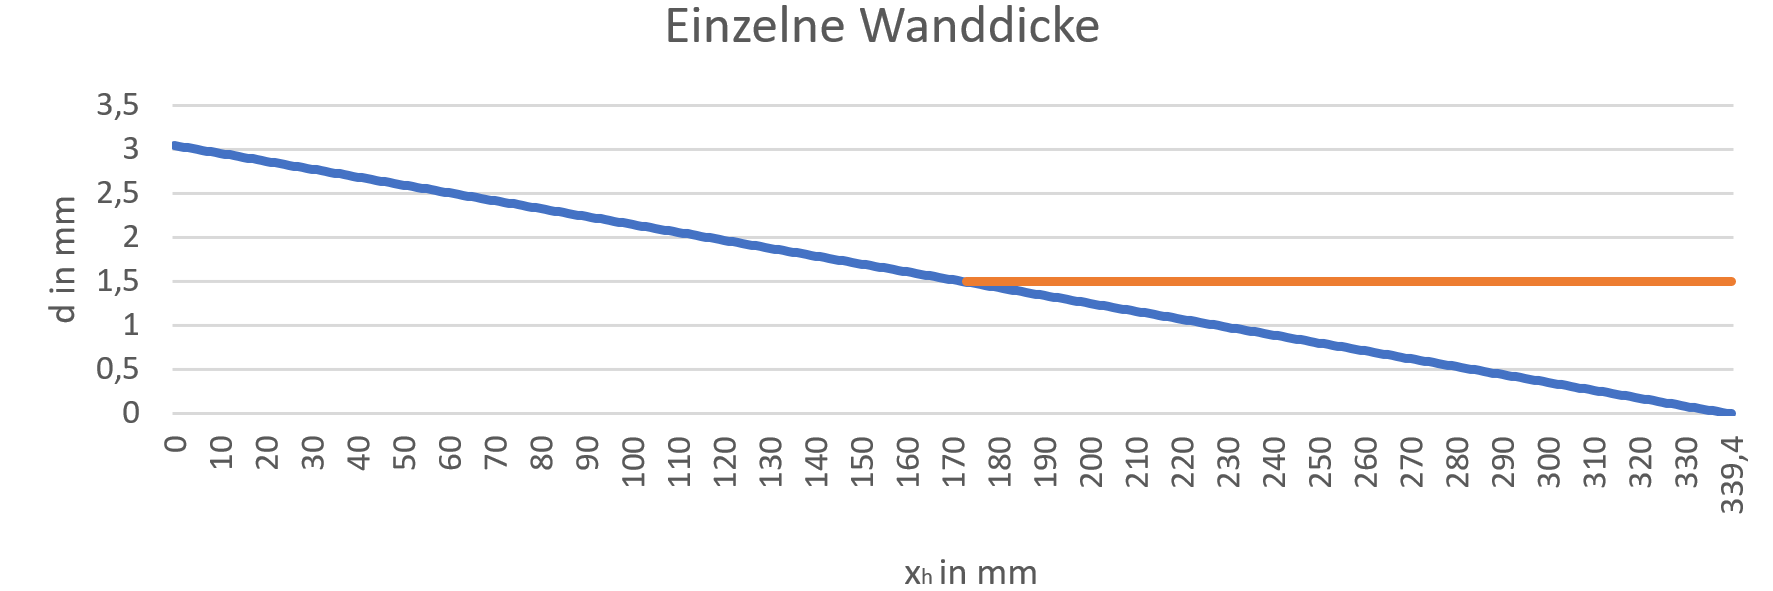
\includegraphics[width=0.85\textwidth]{d_einzel.png}
	\caption{Der Verlauf der Wanddicke $d$ in Abhängigkeit von $x_h$}
	\label{abb_d_einzel}
\end{figure}\\
Da das Moment unter diesen einfachen Annahmen am Ende des Grid Fins auf null fällt, errechnet sich dort auch ein Wandstärke von null. Dies ist natürlich kein sinnvolles Ergebnis, sodass eine minimale Wanddicke von $d_\mathrm{min}=1,5$ mm definiert wird. Des Weiteren ist noch zu beachten, dass die Dicke in der Nähe der Einspannung noch höher als dargestellt ist, da dort weniger Wände liegen, auf die die Gesamtdicke verteilt wird.
\\~\\
Nun steht schon mal eine erste Geometrie des Grid Fins, jedoch benötigen auch die zusätzlichen Designelement, die aus dem morphologischen Kasten gewählt wurde Festlegung weitere Werte. Einer davon ist der Pfeilungswinkel $\Lambda_\mathrm{lokal}$. Je größer dieser ist, desto geringer ist die axiale Kraft, doch große Pfeilung schwächt gleichzeitig die Sehne in den Tälern. Also Kompromiss wird der Pfeilungswinkel variiert. An den \textbf{Spitzen} soll ein $\mathbf{\Lambda_\mathrm{lokal}=70^\circ}$ gelten in den Tälern jedoch nur $\Lambda_\mathrm{\textbf{lokal}}=20^\circ$. Der Berg soll $20$mm höher liegen als das Tal und verbunden werden sie über einen Tangentenbogen. Die Fläche dieser Pfeilung entspricht einem Rechteck gleicher Breite mit der Höhe $7$mm. Um also auf eine Sehnenlänge von $s=40$mm zu kommen, muss sich noch $33$mm restliche Wand unter der Pfeilung befinden.

Der Wandquerschnitt spitzt sich auch zu und der zugehörige Winkel wurde für das Gitter auf $70^\circ$ gesetzt. Die Position in wieder so gewählt, dass die durchschnittliche Sehnenlänge sich immer auf dem Wert befindet, der durch die lokale Pfeilung herrschen sollte. Die Rahmenwände haben nur auf einer Seite eine schräge. Der Winkel wurde hier auf\ $54^\circ$ herab gesetzt, sodass Rahmen und Gitter bei gleicher Wandstärke und Sehnenlänge, die selbe maximale Höhe haben.
\begin{figure}[h]
	\begin{minipage}[t]{0.45\linewidth}
		\centering
		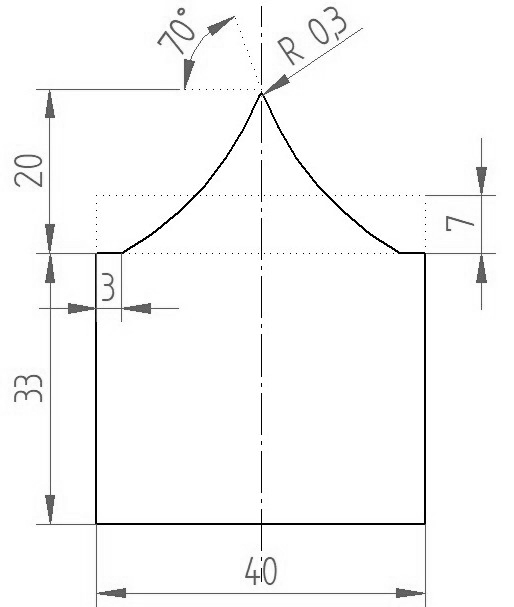
\includegraphics[width=0.85\textwidth]{Pfeil_lok.png}
		\caption{Die Geometrischer Zusammenhänge einer gepfeilten Zellwand}
	\end{minipage}
	\hfill
	\begin{minipage}[t]{0.45\linewidth}
		\centering
		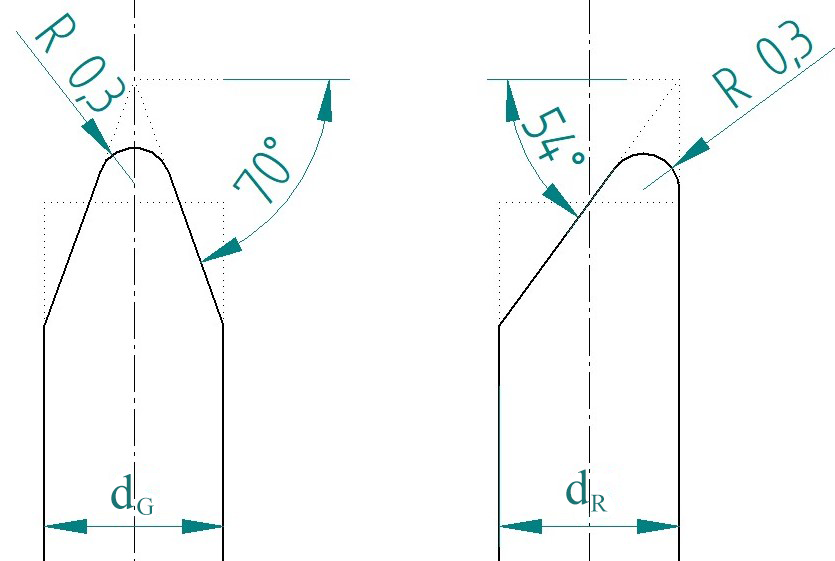
\includegraphics[width=\textwidth]{Wandquerschnitt.png}
		\caption{Zuspitzung der Wände im Querschnitt}
	\end{minipage}
\end{figure}\\
Die Krümmung soll für die Vorderkante der nominellen Sehne ausgelegt werden, also für den Fall, dass keine Pfeilung oder Zuspitzung vorliegt (gepunktete Linie). Da an den Bergen der Pfeilung die Spitze $13$mm und mit der Zuspitzung bei eine Wandstärke von $4$mm einen weiteren Millimeter über der nominelle Sehne liegt, müssen noch mindestens $14$mm auf die $550$mm Raketenradius drauf addiert werden. Somit wird der Krümmungsradius auf $570$mm gesetzt.
\\~\\
Es sind noch weitere Optionen möglich, mit denen sich die Grid Fins modifizieren lassen würden. Diese werden hier jedoch zunächst nur kurz vorgestellt und erst nach den ersten Analysen beurteilt, ob sie eventuell doch noch implementiert werden sollen.

Die additive Fertigung des Grid Fins ermöglicht neue Optionen, die für klassische Herstellungsverfahren nicht wirtschaftlich umsetzbar sind. So können zum Beispiel Kanäle in das Material integriert werden, welche genutzt werden können, um den Werkstoff zu kühlen oder gar das Air Flush System mit weiteren Drucksensoren ergänzen. Es wäre auch denkbar diese einfach nur zur weiteren Gewichtsreduzierung zu nutzen.

Auch denkbar ist es die scharfen Kanten, die senkrecht zur Strömung liegen, abzurunden und so einen besseren Kraftfluss zu erlauben.
\\~\\
Zum Schluss muss an dieser Stelle noch angemerkt werden, dass 3D-Drucker natürlich nur eine begrenzte Auflösung haben. Je nach Hersteller kann somit die minimale Wandstärke $0,4-1,0$mm \cite{eos, preise} und die Schichtdicke $0,04-0,075$mm \cite{preise} betragen. Die Ausrichtung im Drucker hat also auch Einfluss auf den Detailgrad. Somit kann es sein, dass die spitzen Kanten und die Pfeilung in der Fertigung stumpfer werden, als sie ausgelegt wurden. Auch das Hinzufügen von Kanälen ist nur möglich, wenn die Wände dick genug sind.
\section{Modellierung des Modells}
  \chapter{Systemanalyse}\label{sec:simulation}
Nachdem nun im vorherigen Kapitel ein erstes Modell mitsamt Aktuatorik entwurfen wurde, soll nun überprüft werden, ob dieses unter Last zum einen genügend Festigkeit besitzt und zum anderen, ob die Aktuatorik auch die entsprechenden Leistungen liefern kann. Auf Basis dieser Analysen werden anschließend Optimierungen der in Kapitel \ref{sec:modellentwurf} getroffenen Entscheidungen vorgenommen.


\section{FEM-Analyse}
Solid Edge bietet direkt das integrierte FEM-Program "NX Nastran" an, was einen schnellen Designzyklus von berechnen und Modell bearbeiten ermöglicht. Für eine effiziente FEM-Analyse werden die Modellvarianten zunächst vereinfacht, indem die Verrundungen und Anschrägungen der Wände entfernt werden. Auch einige der steilen Spitzen der Pfeilung werden abgerundet, da diese bei der Vernetzung nur zu Problemen führt und die Belastungen im Material so gut wie gar nicht verändern.

Bevor dir Kräfte aus Formel \ref{eq_Fmax} und \ref{eq_Fmax2} auf die Geometrie angewandt werden können, müssen sie noch aus dem körperfesten in ein Grid Fin festes Koordinatensystem übertragen werden. Dieses ist in Abbildung \ref{abb_gitter} dargestellt und wurde so definiert, dass die Kräfte $F_2$ und $F_3$ genau normal auf den Gitterwänden stehen, sodass sie sich einfach in der FEM-Analyse implementieren lassen. $F_1$ ist parallel zur Sehne und kann somit, genau wie die anderen beiden Kräfte, gleichmäßig auf alle Flächen verteilt werden, die eine Normale haben, die zum Teil in diese Richtung zeigt.
\begin{figure}[h] 
	\centering
	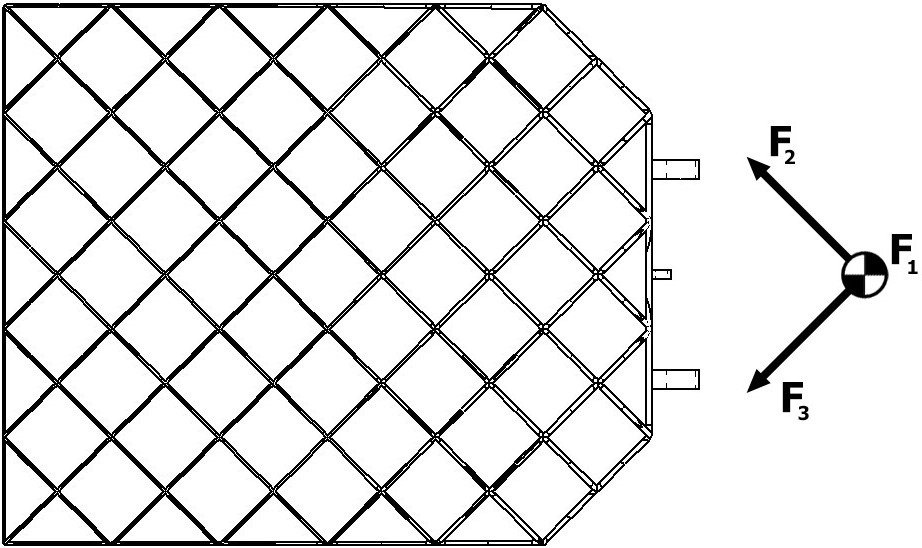
\includegraphics[width=0.9\textwidth]{Gitter.jpg}
	\caption{Kräfte im Grid Fin festen Koordinatensystem}
	\label{abb_gitter}
\end{figure}\\
Somit ergeben sich die Kräfte für die einzelnen Grid Fins zu:
\begin{table}[h]
	\centering
	\begin{tabular}{c||c|c|c|c}
		&D1&R1&D2&R2\\
		\hline
		$F_1/$N&$413,5$&$389,3$&$389,3$&$413,5$\\
		$F_2/$N&$6276,0$&$4970,8$&$-4970,8$&$-6276,0$\\
		$F_3/$N&$4934,0$&$6474,2$&$-6474,2$&$-4934,0$\\
	\end{tabular}
\end{table}
Als Randbedingung werden die Innenflächen der Halterung zylindrisch festgelegt. Das heißt die dort liegenden Knoten können sich weder axial noch radial bewegen, jedoch um die Achse drehen.
\subsection{Optimierung der Halterung}
Bei beiden Pfeilungstypen lässt sich für alle Lastfälle sofort erkennen, dass es zu massiven Lastspitzen an der Halterung kommt. Währenddessen bleiben die Werte im Gitter deutlich niedriger. Der Grund für die hohen Spannungen an der Einspannung ist die ungünstige Lage in der Mitte der Wände anstatt der Schnittstellen, Somit bilden sich vergleichsweise hohe Biegemomente in den Wänden aus. Dieser ungünstige Kraftfluss wird durch die scharfen Kanten weiter verschlimmert. Um nun diese Spannungsspitzen zu vermeiden, sollte, neben einer Abrundung der Kanten, die Position der Halterungen verändert werden.
\begin{figure}[h] 
	\centering
	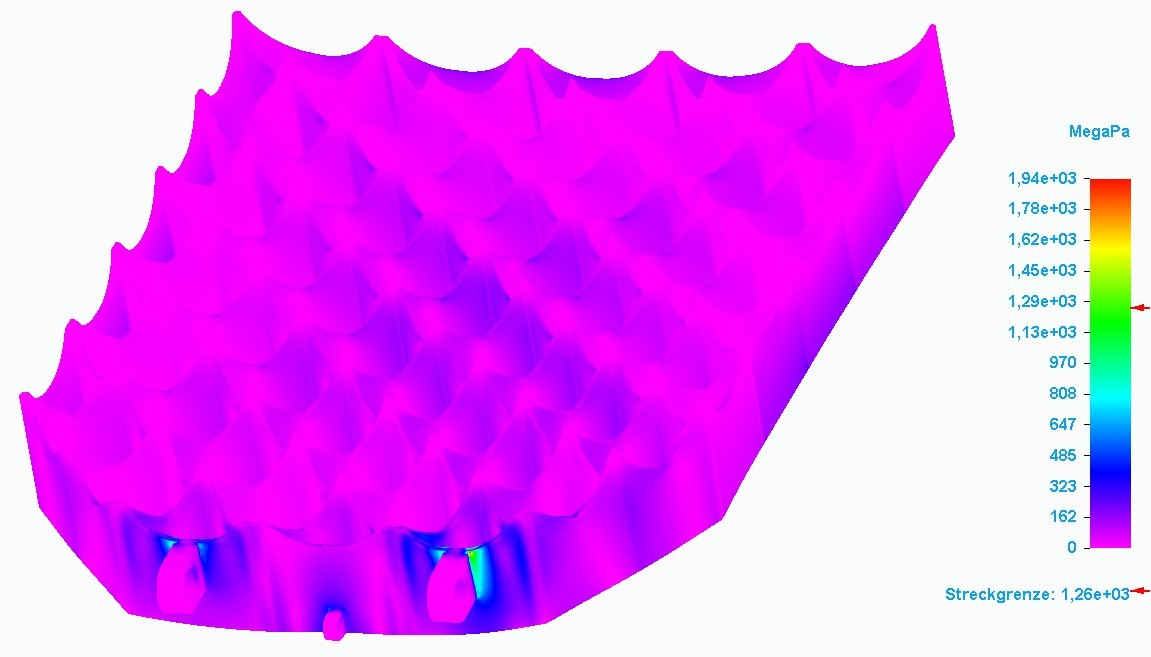
\includegraphics[width=0.9\textwidth]{D1 3.3b max 1.jpg}
	\caption{Maximale Spannungen am Grid Fin D1}
\end{figure}\\
Da sich die Anbringung der Halterungen genau ein der Mitte Zelle befinden, auch wenn sie in diesem Fall halbiert sind, lassen sie sich entweder tangential oder normal zum Raketenkörper verschieben, um sie auf einen Schnittpunkt der Wände zu legen. Soll Halterung B nicht in zwei Teile aufgeteilt werden, so kommt nur eine Bewegung senkrecht zum Körper in Frage. Anstatt die Halterung nun in das Gitter hinein zu legen, was zu einer Verkleinerung der durschdtrömten Querschnittfläche führen würde und somit geringer Normalkräfte, werden zwei der Wände weiter fortgesetzt. Diese schneiden sich dann in der Mitte, wo die Halterung B platziert wird. Die Halterung wird jedoch nicht direkt an der Schnittstelle konstruiert, sondern noch ein bisschen weiter vom Gitter entfernt, sodass die Kraft gradliniger über die Beiden Hubstangen geleitet werden kann.

Für die Halterungen A passiert das gleiche. Die nebenliegenden Gitterwänder werden bis zu ihrer Schnittstelle fortgesetzt. Im Gegensatz zur Halterung B befindet sich jedoch direkt hier die Bohrung, an der das Grid Fin montiert werden soll.
\begin{figure}[h]
	\begin{minipage}[t]{0.45\linewidth}
		\centering
		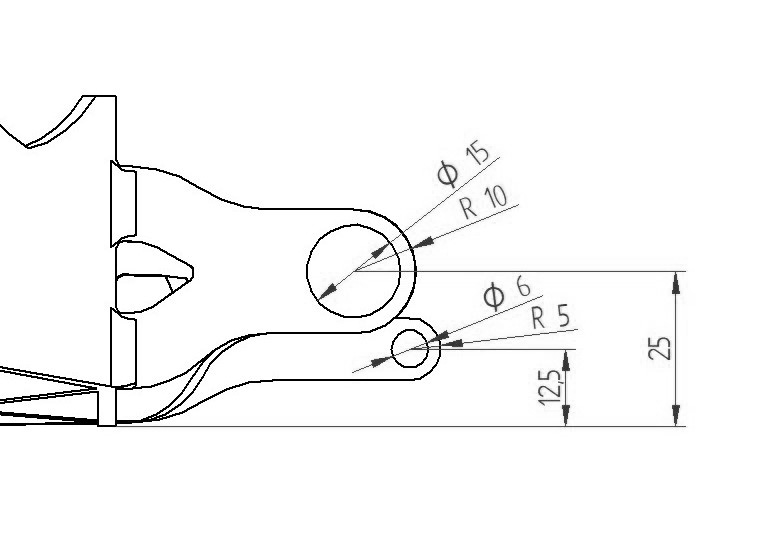
\includegraphics[width=0.85\textwidth]{Skizze Halterung 2.0 1.jpg}
	\end{minipage}
	\hfill
	\begin{minipage}[t]{0.45\linewidth}
		\centering
		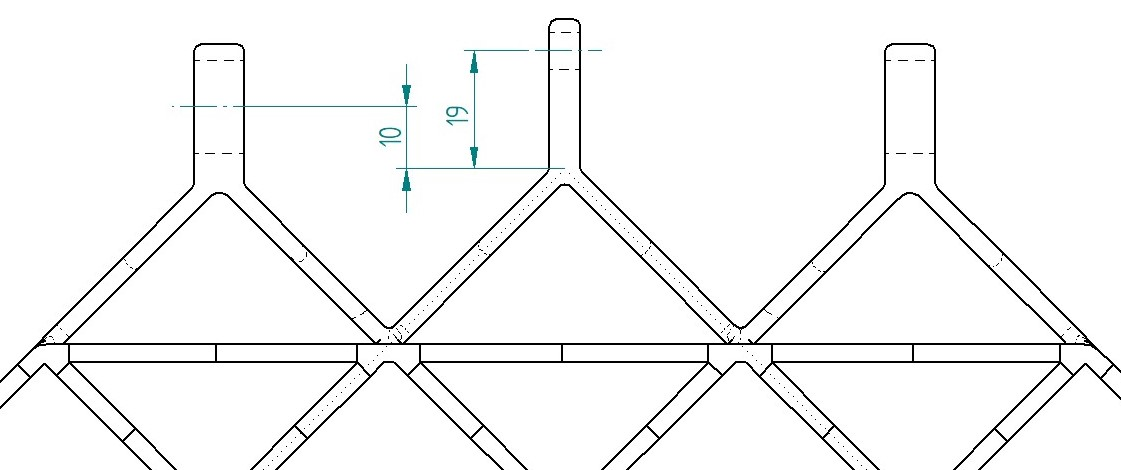
\includegraphics[width=1\textwidth]{Skizze Halterung 2.0 2.jpg}
	\end{minipage}
	\caption{Verbesserte Version der Halterung (1)}
\end{figure}\\
Dies sorgt zwar schon für eine deutlichere Verbesserung, jedoch ist der Hebelarm trotz der Versetzung der Halterung B recht kurz. Dies sorgt dafür, dass dort direkt an der Bohrung noch immer Spannungsspitzen auftreten, die die Streckgrenze von $R_{p, 0.2} = 1262$MPa unterschreiten.
\begin{figure}[h] 
	\centering
	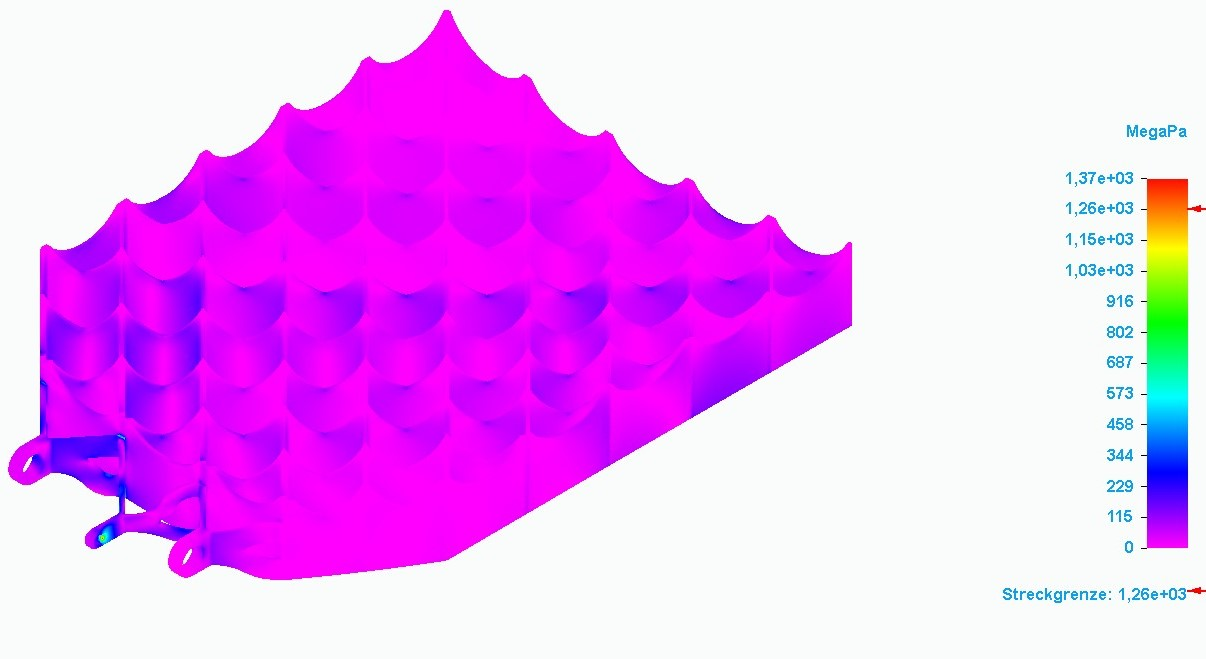
\includegraphics[width=0.9\textwidth]{D2 3.4 b max.jpg}
	\caption{Maximale Spannungen am Grid Fin D2 bei veränderter Halterung(1)}
\end{figure}\\
Um dem Hebelarm zu Verlängern wird nun die Halterung B auf die Höhe der konvexen Seite gebracht. Sie wird außerdem in einer geschwungen Form noch weiter nach vorne gelegt, damit die Verbindungslinie der beiden Halterungen im $45^\circ$ Winkel zur Gitterebene liegt. Dadurch ist die Klappbewegung möglichst gleichmäßig, was den Aktuator schont und gleichzeitig garantiert, dass der Verfahrweg minimal für den gegeben Hebelarm ist.
\begin{figure}[h] 
	\centering
	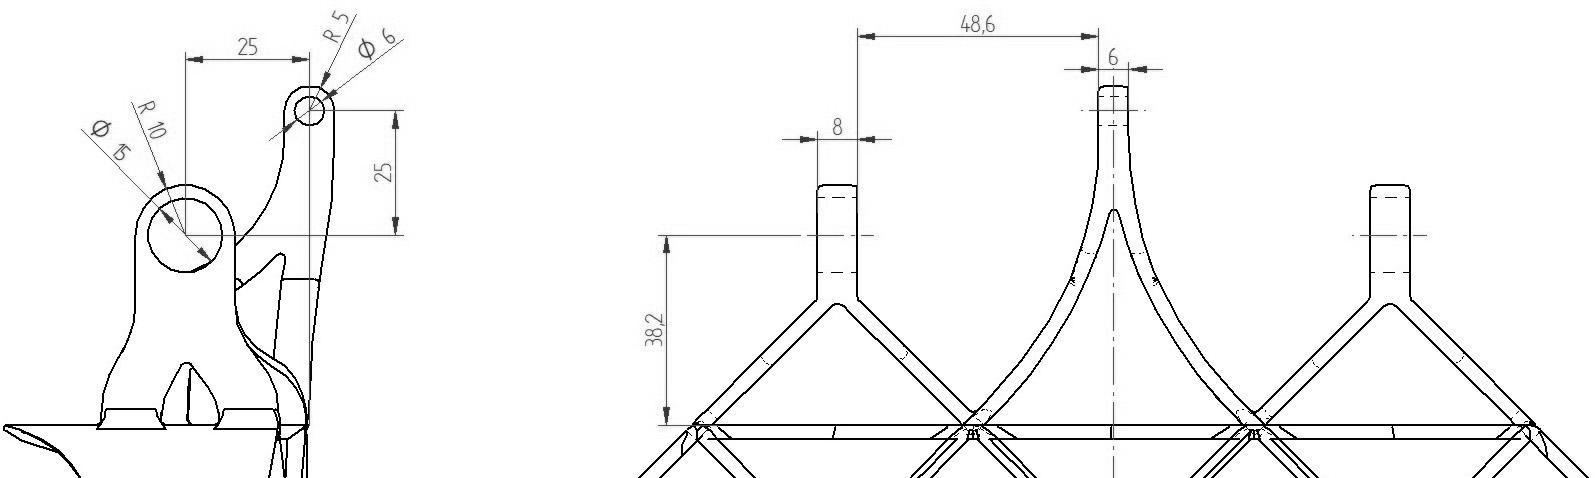
\includegraphics[width=0.9\textwidth]{Skizze Halterung 3.5.jpg}
	\caption{Verbesserte Version der Halterung (2)}
\end{figure}\\
Dies hat nun endlich den gewünschten Effekt, dass die Spannung im Material deutlich niedriger werden. Bei allen Grid Fins treten nur noch Spannungen auf die deutlich unter der Streckgrenze des Materials liegen und somit den Belastungen im Einsatz standhalten.
\begin{figure}[h] 
	\centering
	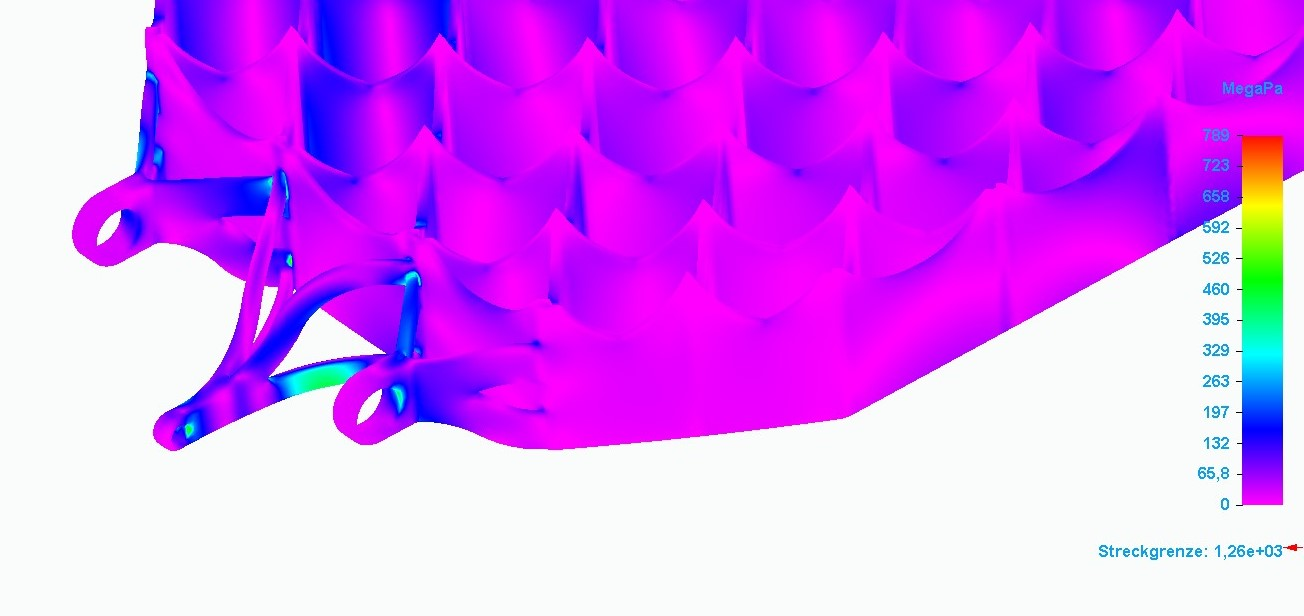
\includegraphics[width=0.9\textwidth]{3.5 b Halterung max.jpg}
	\caption{Maximale Spannungen am Grid Fin D2 bei veränderter Halterung (2)}
\end{figure}\\
Somit wäre die Auslegung der Halterung nach den aerodynamischen Kräften theoretisch abgeschlossen, jedoch muss hierbei auch noch auf die Aktuatorik und das maximale Lastenvielfache geachtet werden. Aktuell hat der Grid Fin eine Masse von $m = 3,5$kg und der Massenschwerpunkt liegt $185$mm von der Halterung A entfernt. Mit dem Lastenvielfachen von ca. 20 beim auslösen des Ballutes entsteht nun also ein Moment von ungefähr $M=127Nm$, welches von der Halterung B kompensiert werden muss. Die Halterung B ist an der Spindelstange montiert und leitet somit die Kraft an diese weiter. Der Hebelarm der Halterung B und die maximale ertragbare Axialkraft der Spindel müssen also aufeinander abgestimmt sein. Maxon Motoren stellt nur Spindeln mit Axiallasten von bis zu $2700$N her, welche folglich einen Hebelarm von $\frac{127Nm}{2700N}=47mm$ erfordert, was noch gerade so für den Grid Fin annehmbar ist. Der Wert liegt laut dieser Rechnung zwar minimal drüber jedoch wird das Lastenvielfache von 20 gar nicht wirklich erreicht, sodass die Rundung annehmbar ist. Da die Hubstange gelenkig mit dem Grid Fin verbunden ist, ist zu beachten, dass nur der Abstand der Haltungen in Sehnenlänge als effektiver Hebelarm wirkt. Somit muss die Halterung B nicht länger weiter vorne positioniert sein, was Material spart. Wird die Verbindungsstange zwischen Halterung und Hubstange auf die gleiche Länge wie der Hebelarm gesetzt, verlängert sich auch nicht der Hub und da die Hubstange nun weiter außerhalb der Rakete im eingeklappten Zustand befindet, braucht sie auch weniger Platz innerhalb der Rakete, wenn der Grid Fin ausklappt. Um auf den gewünschten Hebelarm zu kommen werden nun beide Halterungen noch ein wenig nach außen gelegt, sodass sich die endhültige Geometrie, wie sie in Abbildung \ref{abb_Halterung-fertig} zu sehen ist, ergibt.
\begin{figure}[h] 
	\centering
	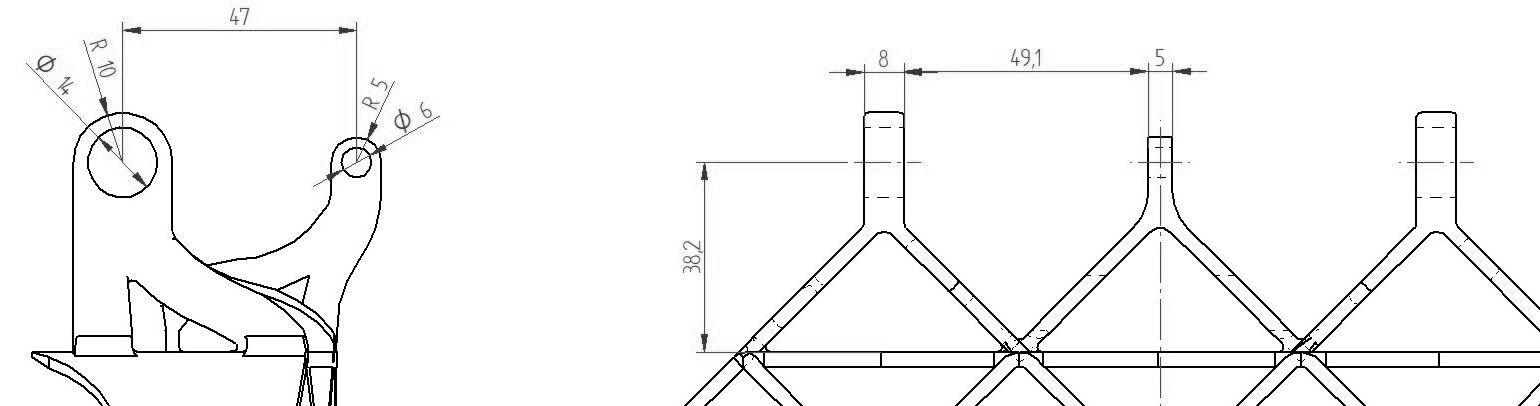
\includegraphics[width=0.9\textwidth]{Skizze Halterung 3.6.jpg}
	\caption{Endgültige Geometrie der Halterung}
	\label{abb_Halterung-fertig}
\end{figure}\\
Zur Bestätigung werden wieder FEM Analysen durchgeführt und diesmal werden ergänzend zu den aerodynamischen Kräften auch in einem separaten Lastfall die Beschleunigungskräfte untersucht. Bei den Lastvielfachen werden die anderen Kräfte ignoriert, da sie eher eine Stützwirkung habe und somit die Spannungen nur weiter senken würde. Beim Auftreten der Ruckartigen Abbremsung durch den Ballonschirm ist der Max Q sowieso schon überschritten uns somit die anderen Kräfte nur noch deutlich geringer. Wie Abbildungen QQQQQQQQQQQQQQ und AAAAAAAAA zeigen wird die Streckgrenze weiterhin nicht unterschritten. Somit gibt die Halterung als bestätigt.
\subsection{Optimierung des Gitters}
Als nächstes wird das Gitter untersucht. Es ist sofort erkenntlich, dass die Belastungen überall relativ niedrig, deutlich unter der Streckgrenze, liegen. Egal ob beim Tal- oder Berg-Typus, die Spannungsspitzen, die auftreten, sind keines Wegs kritisch. Somit ist eine Aufdickung des Material nicht nötig, sondern es kann über eine Reduzierung der Wandstärke nachgedacht werden.

Die Wanddicke ist jedoch nicht nur durch die mechanische Belastung, sondern auch die thermische, nach unten hin beschränkt. Diese ist jedoch ein sehr komplexes Phänomen, das von der Zusammensetzung der Atmosphäre, den zeitlich ändernden Strömungsbedingungen, die Postion des Verdichtungsstoßes und dem Aufbau des Grid Fins abhängen, sodass es nicht auch nur überschlägig in dieser Arbeit behandelt werden kann.
\\~\\
Der Grid Fin ist momentan am von der Rakete weg zeigenden Ende schon nur $1,5$mm dick, was für den Wiedereintritt schon ein relativ kleiner Wert sein könnte. Deswegen soll dieser zunächst nicht unterschritten werden.



~\\~\\
Der Vergleich von der Berg- und Tal-Konfiguration zeigt, 


\section{Bestätigung der Akuatorik}
Nun da die Geometrie des Grid Fins, insbesondere der Halterung fest steht, kann überprüft werden, ob auch alles auf der wellenseitig den mechanischen Lasten stand hält. Hierfür werden die Kräfte, die an den einzelnen Halterungen wirken benötigt. Die detaillierte Rechnung befindet sich im Anhang \ref{sec_halterkraefte}. Wenn angenommen wird, dass die Halterung B, da sie deutlich weniger steif als die Halterungen A sind, nur Belastung in $\eta$-Richtung aufnehmen kann ergeben sich die Kräfte wie folgt. Links sind Kräfte am Grid Fin R1 dargestellt, was die höchste Belastung für das Lager A bedeutet, und rechts R2 mit der höchsten Belastung für Lager B.
\begin{table}[h] 
	\centering 
	\begin{tabular}{c|c|c|cc||c|c|c|c} 
		\textbf{R1}&$F_{\zeta}$[N]&$F_\eta$[N]&$F_\xi$[N]&&\textbf{R2}&$F_{\zeta}$[N]&$F_\eta$[N]&$F_\xi$[N]\\ 
		\hline 
		A1& 612,00&-5601,54&-531,55&&A1&599,90&5,16&-474,45\\
		A2&-1001,31&-1624,49&-531,54&&A2&.1013,41&3554,87&-474,45\\
		B&0&-886,81&0&&B&0&4366,53&0\\
	\end{tabular}
\end{table} \\
Für die Bauteile, die nicht so hohen Lasten wie der Grid Fin ausgesetzt sind, wird im folgenden nicht mit den Werkstoffwerten des teuren Edelstahls 1.4542 gerechnet. Für die Teile, die nicht mit der Strömung in Kontakt kommen, wird eine Aluminiumlegierung mit $R_{p,0.2} = $MPa verwendet, und für die anderen Bauteile, wie weiterhin auch hohen thermischen Lasten ausgesetzt sind, wird ein Edelstahl mit einer Streckgrenze von $R_{p,0.2} = 400$MPa angenommen.
\subsection{Lager der Halterung}
Für die Lasten an den Lagern ist nur die Aufteilung in Radial- $F_r$ und Axialkraft $F_a$ von Bedeutung. Dabei sei noch zu bedenken, dass die Kraft in $\xi$-Richtung auf Grund des Aufbaus nur von einem der A Lager kompensiert werden kann. Auch wenn das für die vorherige Berechnung keine Rolle spielte, da die beiden Halterungen A auf einer Achse liegen, wird es im folgenden berücksichtigt.
\begin{table}[h] 
	\centering 
	\begin{tabular}{c|c|cc||c|c|c} 
		\textbf{R1}&$F_{r}$[N]&$F_a$[N]&&\textbf{R2}&$F_{a}$[N]&$F_r$[N]\\ 
		\hline 
		A1& 5634,87&-1063,10&&A1&599,92&948,90\\
		A2&1908,29&0&&A2&3696,60&0\\
		B&866,81&0&&B&4366,53&0\\
	\end{tabular}
\end{table} \\
Aus diesen Werten lässt sich nun über die Flächenpressung und Abscherung den erforderlichen Durchmesser $D$ und die benötigte Auflagebreite $B$ der Hilfswelle bestimmen. Für die Abscherung git
\begin{equation}
	\tau_{\mathrm{zul.}}\leq\tau_\mathrm{scher}=\frac{F_r}{m\pi D^2/4}.
\end{equation}
Mit $\tau_{\mathrm{zul.}}=R_{p, 0.2}\cdot 0,6$ \cite{metall} und $m$ als die Anzahl der Schnittflächen lässt sich der Mindestdurchmesser bestimmen.
\begin{equation}
	D \leq \sqrt{\frac{4F}{m\pi 0,6 R_{p, 0.2}}}= 5,5\mathrm{mm}
\end{equation}
Für die Halterung A ist $m=1$, sodass eine Mindestdicke von $D=5,5$mm benötigt wird. Aus der sich eine Auflagebreite von $B = 3,1$mm ergibt. Da sich der Aufbau des Grid Fins seit dem ersten Modell verändert hat, kann auch die Anbringung an der Welle, welche in Abbildung \ref{abb_Welle} zu sehen war, angepasst werden. Durch wie Verlegung der Halterung A rückt der Grid Fin näher an den Raketenkörper ran. Statt nun Greifarme aus der Welle raus ragen zu lassen, wir diese nur ein wenig verlängert, sodass die Verbindungslinie durch die beiden Halterungen A die Welle durchstößt. Auf diese Verbindungslinie wird eine Stange, im weiteren Verbindungswelle genannt, gelegt, auf der der Grid Fin montiert wird. Diese Variante der Halterung hat zum einen den Vorteil, dass keine komplizierte Greiferstruktur gefertigt werden muss, und zum anderen steht nun ein Großteil der planaren Wand im eingeklappten Zustand nicht mehr direkt in der Strömung, sondern im Windschatten der Welle. Dadurch wird ungewollter Widerstand und Belastung der Grid Fins verhindert. Um den Grid Fin reibungsarm zu sicher, muss er sowohl axial als auch radial mit Wälzlagern gelagert werden. Zylinderrollenlager, wie sie auch bei der Welle verwendet werden, sind hier jedoch eine ungünstige Wahl, da sie recht großen Bauraum benötigen. Stattdessen wird die Halterung A auf beiden Seiten mit einem schmalen Nadellager radial und mit einem Kugellager axial mit der Welle verbunden. Diese Kombinationslager werden von außen mit Nutmuttern, die auf die Verbindungswelle aufgeschraubt und durch Sicherungsbleche gesichert werden, an den Grid Fin gedrückt. Um ein Verrutschen der Verbindungswelle in der Welle zu verhindern, muss diese noch durch eine Passschraube fixiert werden. Für diese Passschraube werden wieder aus der Flächenpresssung und der Abscherung die Mindestmaße des Durchmessers und der Breite bestimmt. Mit eim Durchmesser von $D = 10\mathrm{mm}> 1,2$mm und einer Kontaktbreite von $B = 8\mathrm{mm}> 1,3$mm ist sie für diese Anwendung ausreichend.
\begin{figure}[h] 
	\centering
	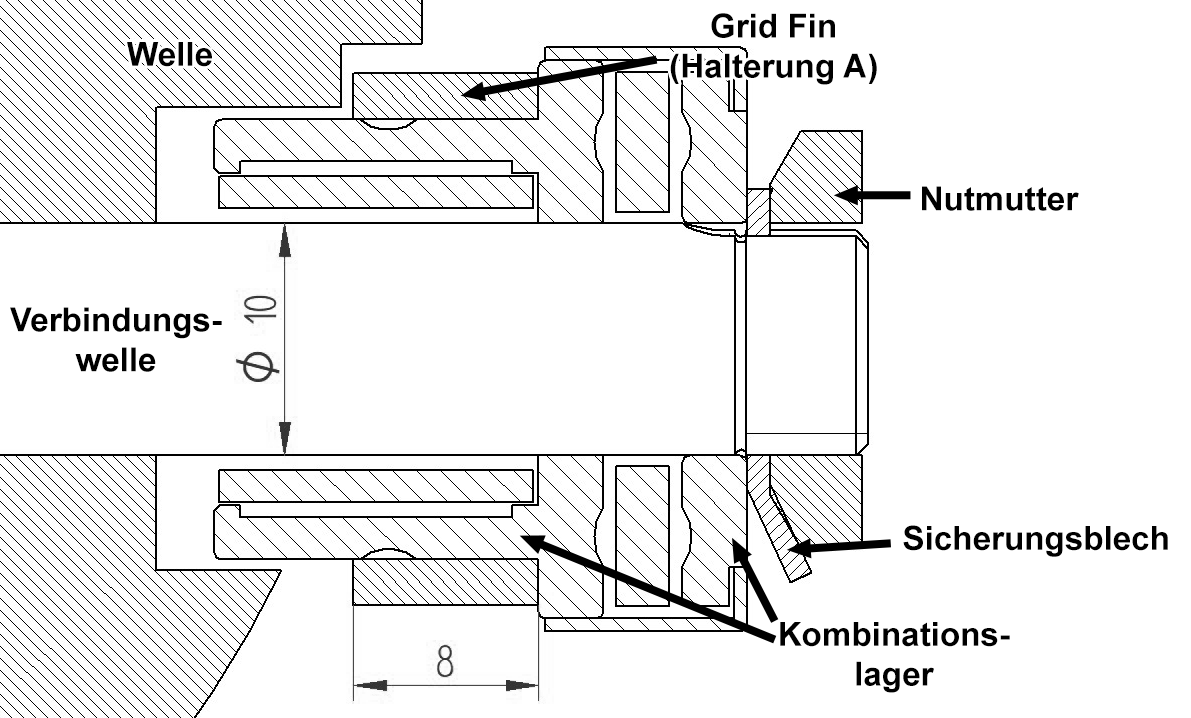
\includegraphics[width=0.75\textwidth]{Skizze Halterung A.png}
	\caption{Lagerung der Halterung A}
\end{figure}\\
Die Halterung B wird von beiden Seiten gestützt, sodass mit $m = 2$ ein Mindestdurchmesser von $D = 3,4$mm errechnet wird. Die zugehörige Breite beläuft sich somit auf $B = 3,8$mm. Wie schon angemerkt treten hier kaum Axialkräfte auf, sodass ein Rillenkugellager ausreicht, um diese aufzunehmen. Es wird auf der einen Seite gegen eine Schulter in der Halterung B des Grid Fins gedrückt und auf der anderen Seite durch ein Sicherungsring fixiert. Zwei Stifte werden von beiden Seiten gegen die innere Kante des Lagers gedrückt und miteinander schraubt. Diese Stifte können anschließend von außen mit Muttern an die Verbindungsstange für den Hub fixiert werden. Somit ist auch die Halterung B Axial und Radial bestimmt, kann sich aber noch immer reibungsarm um ihre Achse drehen. Das Kugellager hat zwar nur eine Breite von 3mm, was unter dem Wert liegt, der sich aus der Flächenpressung ergeben hat. Jedoch wurde dort mit dem Mindestdurchmesser gerechnet, sodass, wenn mit dem Innendurchmesser des Kugellagers von $D = 5$mm die Rechnung wiederholt wird, nur noch eine Breite von $B =2,6$ benötigt wird. Diese Lagerung wird genau so auch ein zweites Mal auf der anderen Seite der Verbindungsstange verwendet.
\begin{figure}[h] 
	\centering
	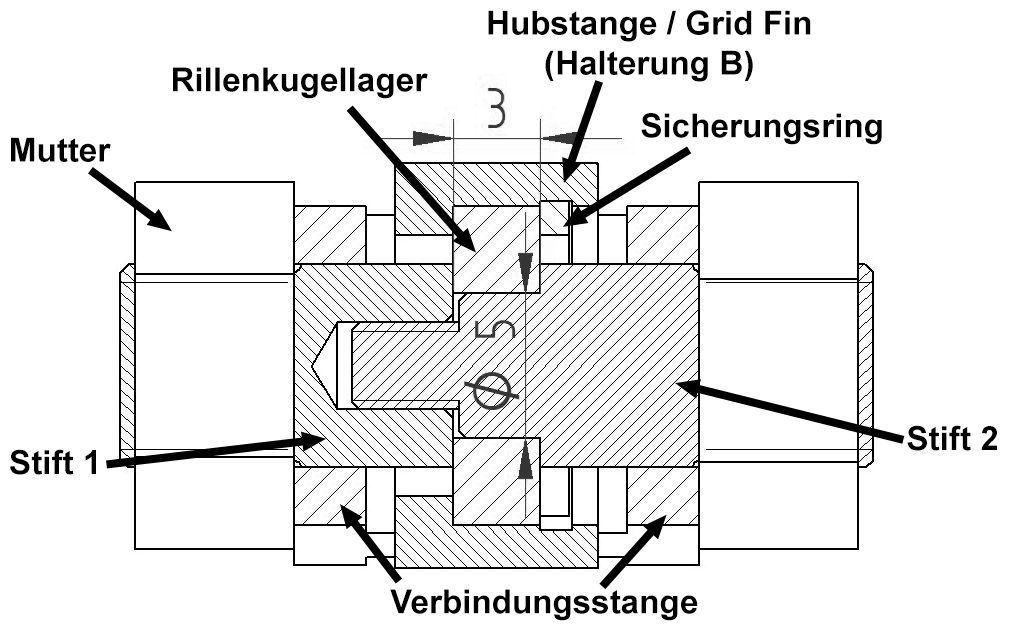
\includegraphics[width=0.75\textwidth]{Skizze Halterung B.png}
	\caption{Lagerung in der Halterung B}
\end{figure}
\subsection{Lagerung der Welle}
Als nächstes wird die Lagerung der Welle überprüft, da diese sich auch unter Last bewegen müssen. Hierzu werden zunächst über das Kräftegleichgewicht die Lasten in den beiden Kegelrollenlagern bestimmt.
\begin{figure}[h] 
	\centering
	\includegraphics[width=0.9\textwidth]{Skizze Lager.png}
	\caption{Lagerkräfte an den Kegelrollenlagern}
\end{figure}\\
Für den Fall, dass die am Grid Fin angreifende Axialkraft in positive $\eta$-Richtung zeig, ist die Axialkraft am vorderen Kegellager $F_{a, \mathrm{K1}} = 0$ und am hinteren $F_{a, \mathrm{K2}} = F_\eta$. Da es für den anderen Fall genau umgekehrt ist, wird bei der Untersuchung der maximalen Belastung für beide Lager angenommen, dass sie die Axiallast aufnehmen. Die Radialkräfte ergibt sich aus der Kraft in $\zeta$- und $\xi$-Richtung und lässt sich mit dem Kräfte- und Momentengleichgewicht bestimmen.
\begin{equation}
	F_{r, \mathrm{K1}} = F_r\cdot\frac{208\mathrm{mm}}{265\mathrm{mm}}=6359,5\mathrm{N}
\end{equation}
\begin{equation}
	F_{r, \mathrm{K2}} = F_r-F_{r, \mathrm{K1}}=1742,7\mathrm{N}
\end{equation}
Aus den Lasten in den Lagern und den in den Herstellerangaben genannten statischen Tragzahlen lässt sich die äqivaltene Belastung berechnen. Mittels der ebenfalls vom Hersteller gegebenen dynamische Tragzahl ergibt sich für beide Lager eine Lebensdauer vom mehreren tausend Stunden \cite{metall}. Es wurde dabei mit der maximal auftretenden Drehzahl, die sich aus der in Kapitel \ref{sec:betriebssim} beschriebenen Betriebssimulation ergibt, gerechnet. Trotzdem liegt der Wert noch immer deutlich über der benötigten Lebensdauer. Dies liegt jedoch daran, dass die große der Lager sich aus der Geometrie der Welle und des Grid Fins ergeben hat, wodurch kein kleines Modell in Frage kommt und bei den gewählten Exemplaren wurde schon versucht die preislich günstigste Option zu wählen.
\subsection{Belastung der Welle}
Die Welle selbst hat zum einen den groben Verlauf, wie er in Abbildung \ref{abb_Welle} zu sehen war, zum anderen weicht sie an einigen Stellen von dieser rotationssymmetrischen Geometrie ab. Ein Aspekt ist die schon im Abschnitt zu der Halterung angesprochenen Verbindungswelle, die die Welle durchstößt. Auf der gleich Höhe, aber auf der Stirnseite befindet sich Mittig eine Bohrung und Senkung für die Passfeder. Für die Hubstange befindet sich des Weiteren ein großer Ausschnitt durch den größten Durchmesser der Welle. Damit im eingeklappten Zustand die Berge des Grid Fins nicht gegen die Welle stoßen, ist die untere Vorderkante ausgehöhlt. Das Linearlager der Hubstange muss von unten festgeschraubt werden, sodass zunächst ein flacher Ausschnitt in die Welle eingebracht wird, auf der eine Platte festgeschraubt werden kann. Diese Platte wird anschließend von unten mit dem Lager verschraubt. Um ein montieren der Schrauben zu ermöglichen werden jedoch noch Einbuchtungen an der Welle benötigt. Von den sechs Bohrungen auf der Welle für die Platte sind die hinteren zwei größer Dimensioniert, da dort noch ein weiteres Bauteil montiert werden soll, an dem anschließend die das Spindelgetriebe festschraubt wird.
Für das Spindelgetriebe mit dem integrierten Motor sind auch noch kleine Einbuchtungen in der Welle nötig. Am hinteren Ende befindet sich dann noch das Gewinde für die Nutmutter und die Nut für das Sicherungsblech. Schlussendlich befindet sich an der hinteren Stirnseite der Welle eine Bohrung mit Passfedernut, mit die Welle des Getriebes montiert wird.
\begin{figure}[h] 
	\centering
	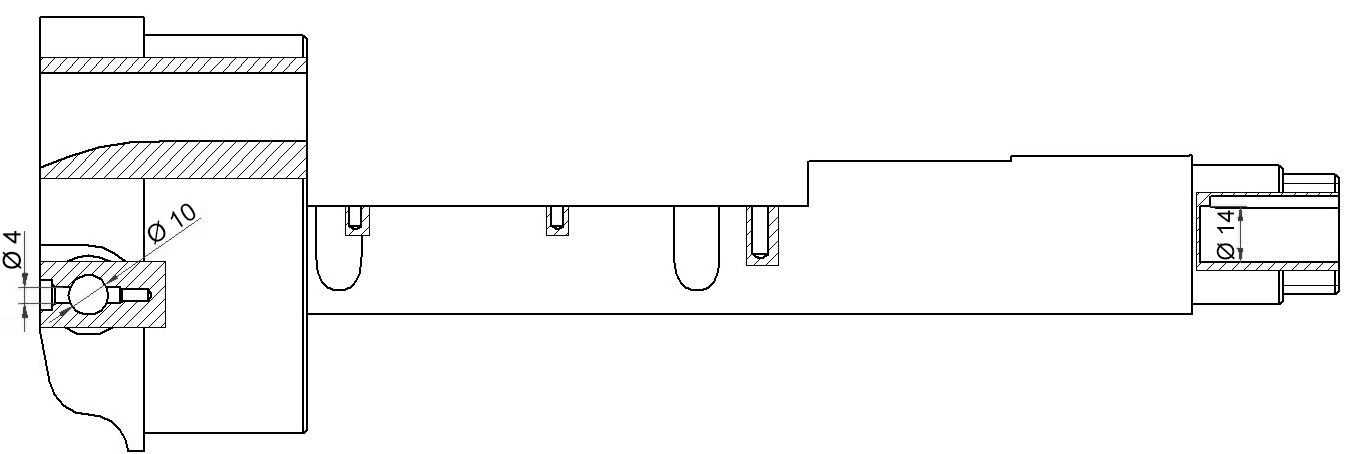
\includegraphics[width=0.9\textwidth]{Skizze Welle ausbruch.jpg}
	\caption{Aufbau der Welle}
\end{figure}\\
Für die Analyse der Welle wurden wieder FEM-Berechnungen durchgeführt. Auf den Flächen, wo die Lager aufliegen, wird wie schon beim Grid Fin zylindrische Bedingungen festgelegt, wobei die axiale Beschränkung nur bei jeweils einem der beiden Lager angewandt wird. Zusätzlich wird ein Drehung der Welle um ihre Achse durch ein festhalten in tangentiale Richtung der Passfedernut am hinteren Ende verhindert.
Die Kräfte der Halterung A werden an den Stellen eingeleitet, wo die Verbindungswelle in die Welle führt, mit Ausnahme der $xi$-Kraft, die durch die Passschraube übertragen wird. 
Die Kraft der Halterung B hingegen wird erst über das Spindelgetriebe auf die Welle übertragen. Somit greift die resultierende Kraft in der Simulation in den Bohrlöcher an, an denen die Spindel befestigt ist.
\begin{figure}[h] 
	\centering
	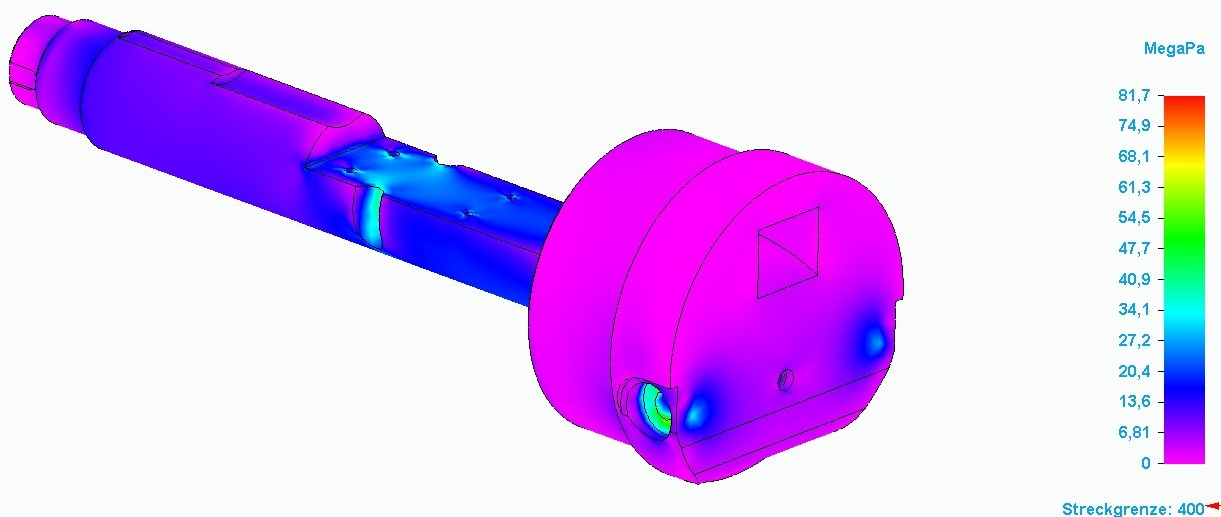
\includegraphics[width=0.9\textwidth]{FEM Welle.jpg}
	\caption{FEM-Ergebnisse der Welle \textbf{UPDATENNNN!!!}}
	\label{abb_Well_FEM}
\end{figure}\\
Wie auch bei den Lagern, ist die Dimensionierung der Welle nicht durch die mechanischen Lasten sondern geometrischen Randbedingungen bestimmt.

\subsection{Belastung des Gehäuse}
Schlussendlich wird noch das Gehäuse betrachtet. Es hat nicht nur die Aufgabe den Rest der Rakete von den beweglichen Teilen zu trennen, um zum Beispiel ein verfangen von Kabeln zu verhindern, sondern auch die Funktion die Lager und den Motor mit Getriebe in Postion zu halten. Somit überträgt das Gehäuse auch die Kräfte und Momente die in dem System wirken auf den Raketenkörper. Für eine einfache Montage und Fertigung besteht das Gehäuse aus eine Unter- und Oberseite, die mit Schrauben aneinander und an der Außenhülle befestigt werden. Im vorderen Bereich benötigt die Oberseite der Welle auf Grund der Klappaktuatorik deutlich mehr Platz als auf der Unterseite. Deshalb bildet die Oberseite des Gehäuse einen Halbkreis, während die Unterseite eine Halbe Ellipse darstellt, deren große Halbachse dem Radius der Oberseite entspricht, um bündig mit ihr abzuschließen. Hinter dem Kegelrollenlager sind beide Seiten symmetrisch aufbaut mit Ausnahme der Wände, an denen das Getriebe und der Motor montiert werden. Somit muss bei der Montage als letzter Schritt nur noch die Gehäuseoberseite auf die Unterseite platziert und dann befestigt werden.
Diese Befestigung findet mit der Raketenhülle mit sechs gleichmäßig über einen Flansch verteilte Schrauben statt. Auch miteinander werden die beiden Hälften zunächst über sechs Schrauben, die gleichmäßig verteilt platziert und mit Mutter befestigt werden.
\\~\\
Auch hier wird wieder eine FEM-Anaylse benutzt, um die Spannungen im Material zu bestimmen. Hierbei werden die Lagerkräfte auf die Flächen aufgebracht, auf denen die Lager aufliegen und gegen drücken. Das Moment um die Wellenachse wird über das Getriebe und den Motor auf das Gehäuse übertragen. Da das Getriebe eine Übersetzung von 200:1 besitzt und der Motor nur sehr kleine Momente liefert, wird vereinfacht angenommen, dass das gesamte Moment an Löchern für die Schraube des Gewindes angreift.
\begin{figure}[h] 
	\centering
	\includegraphics[width=0.9\textwidth]{FEM Gehäuse.jpg}
	\caption{Ergebnisse der FEM-Berechnung der Gehäusebaugruppe}
\end{figure}\\
Die FEM-Anaylse zeigt, dass die Beanspruchungen im Material überall recht gering sind. Nur die Schrauben und Mutter werden stark mit Spannungen von bis zu $900$MPa belastet.
\section{Betriebssimulation}\label{sec:betriebssim}
Da nun bewiesen wurde, dass die Konstruktion den mechanischen Lasten des Betriebs stand hält, soll an dieser Stelle überprüft werden, ob die Antriebe über genug Leistung verfügen die gewünschten Manöver durchzuführen. Deswegen wird zur Überprüfung der Aktuatorik Betriebssimulationen in Simulink durchgeführt.
\subsection{Klappwinkel}
Zuerst wird der Prozess des Ausklappens simuliert. Dieses System besteht aus drei Teilen. Das erste Subsystem stellt der Motor dar, dessen Kennlinie sich mit Gleichung \ref{eq_kennlinie} beschreiben lässt.
\begin{equation}\label{eq_kennlinie}
	n =k_nU-\frac{\Delta n}{\Delta M}M_{Motor}
\end{equation}
$k_n$ ist dabei die Drehzahlkonstante des Motors und ist zusammen mit der Kennliniensteigung $\frac{\Delta n}{\Delta M}$ als konstante Kenngröße dem Datenblatt zu entnehmen. Die Spannung $U$ wird von außen angelegt und die Drehzahl $n$ ergibt sich aus der Lösung des Systems, sodass die Gleichung nach dem Motormoment umgestellt werden kann. Dieses Moment wird dann jedoch noch vom Getriebe verstärkt, sodass sich das Antriebsmoment ergibt. Dieses Getriebe besteht zwar sowohl aus der Spindelstange, die die Rotions- in eine Linearbewegung umwandelt, und einem vorgeschalteten Planetengetriebe, jedoch wird im ersten Subsystem nur das Planetengetriebe berücksichtig, während die Spindelstange vorerst ignoriert wird. Das Antriebsmoment wird dann an das zweite Subsystem weiter gegeben, in dem die Differenzialgleichung
\begin{equation}
	I\ddot{\varphi} = M_{Antrieb} - M_{R}(\dot{\varphi})
\end{equation}
gelöst wird. Die Beschleunigung des Trägheitsmoments $I$ um den Verdrehwinkel $\varphi$ hängt also von der Differenz des Antrieb- und Reibmoments ab. Letzteres ergibt sich aus dem Hebelarm $r$ und der Reibkraft, die wiederum vom Reibungsbeiwert $\mu$ und der Normalkraft $F_N$ abhängig ist, des jeweiligen Kontaktpunktes ab und ist immer der Bewegung entgegen gerichtet. Für das Getriebe ist zwar kein Reibungsbeiwert bekannt, aber eine Nenneffizienz $\eta$, sodass das Reibmoment als ein nur vom Antriebsmoment abhängiger Wert angenommen wird.
\begin{equation}\label{eq_reibmoment}
	M_R = M_{Antrieb}\cdot(1-\eta)+\frac{\dot{\varphi}}{|\dot{\varphi}|}\sum F_N \mu r
\end{equation}
Aus dem Ergebnis dieser Differenzialgleichung, die Drehbeschleunigung $\varphi$, lässt sich dann zum einen die Drehgeschwindigkeit $\dot{\varphi}$ mittels einfacher und den Verdrehwinkel $\varphi$ mit zweifacher Integration bestimmen. Die Drehgeschwindigkeit wird zum einen für die Richtung des Reibmoments, wie es in Gleichung \ref{eq_reibmoment} zu sehen ist, benötigt und zum anderen für die Umrechnung zur Drehzahl an den Motor zurück gegeben. Der Verdrehwinkel wird jedoch an das dritte und letzte Subsystem, welches sich mit der Geometrie der Kinematik beschäftigt, weiter geleitet.

Hier wird die Verdrehung über die Steigung der Spindelstange erst in eine Linearbewegung der Hubstange und dann wieder in die Rotation des Grid Fins um den Klappwinkel $\Lambda$ umgewandelt. Abbildung \ref{abb_kinklapp} zeigt, wie aus den geometrischen Zusammenhängen sich zuerst der Winkel $\alpha$ aus dem Hubweg $x$ ergibt, der dann genutzt werden kann, um den $\Lambda$ zu bestimmen.
%\begin{figure}[h] 
%	\centering
%	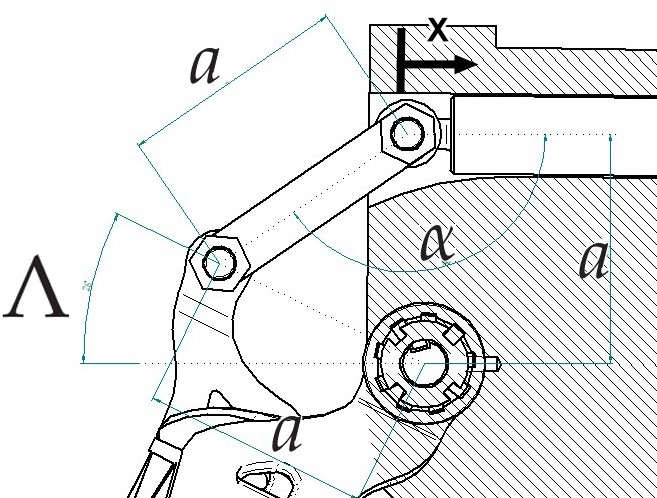
\includegraphics[width=0.9\textwidth]{KinKlapp.jpg}
%	\caption{Kinematischer Zusammenhang von Hubweg und Klappwinkel}
%	\label{abb_kinklapp}
%\end{figure}
\begin{figure}[h] 
\centering
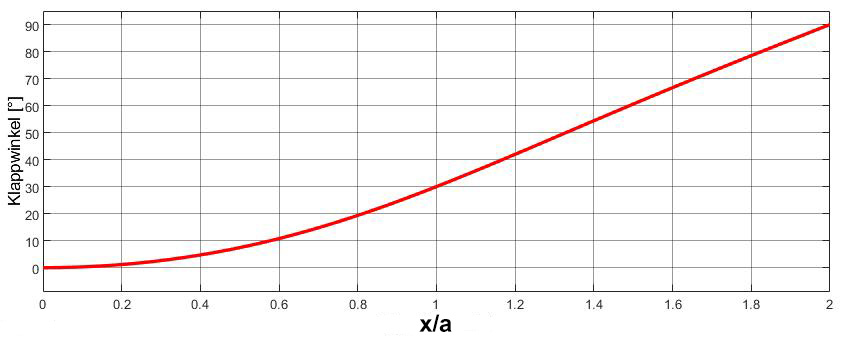
\includegraphics[width=0.9\textwidth]{KinKlappGraph.jpg}
\caption{Klappwinkel in Abhängigkeit vom normalisierten Hubweg}
\end{figure}\\	
Sobald der Klappwinkel von $\Lambda = 90^\circ$ erreicht wird, beziehungsweise wenn die Hubstange sich um eine Länge von $x = 2a = 94$mm bewegt hat, stößt sie gegen die Welle und kann sich nicht weiter in diese Richtung bewegen. Sobald dieser Fall eintritt wird die Spannung am Motor




\subsection{Steurwinkel}
Im Zentrum steht die Differenzialgleichung der Verdrehung des Grid Fins $\delta$, die abhängig vom Moment, dass der Motor liefert, ist. Dieses Moment lässt sich aus der Gleichung
\begin{equation}
	n =k_nU-\frac{\Delta n}{\Delta M}M_{Motor}
\end{equation}
berechnen. $n$ ist hierbei die Drehzahl des Motors, $U$ die Spannung, die am Motor angelegt wird, $\frac{\Delta n}{\Delta M}$ die Steigung der Motorkennlinie und schlussendlich $M_{Motor}$ als das vom Motor erzeugte Moment. Die Größen $k_n$ und $\frac{\Delta n}{\Delta M}$ sind konstante Kenngrößen des Motors und werden vom Herstellen angegeben. Die Drehzahl hingeben ergibt sich aus der Differenzialgleichung des Systems. Das Moment wird anschließend nur noch durchs Getriebe zum Antriebsmoment $M_{Antrieb}$ übersetzt und dann an die Differenzialgleichung übergeben.
\\~\\
Diese ergibt sich nun aus dem Momentengleichgewicht zu:
\begin{equation}
	I\ddot{\delta} = M_{Antrieb} - M_{m, \delta}\delta - M_{R}(\dot{\delta})
\end{equation}
Das Trägheitsmoment setzt sich aus dem des Motors, des Getriebes und des Grid Fins zusammen. Dabei muss das Trägheitsmoment des Motors noch mit der Übersetzung des Getriebes multipliziert werden, da dieser um jenen Faktor stärker beschleunigt. Das aerodynamische Moment wird als linear vom Steuerwinkel abhängig angenommen, was sich bei den Analysen von Miller und Washington \cite{synopsis} (vgl. Abbildung \ref{abb_krumm}) erkennen lässt. Somit ergibt sich $M_{m, \delta} = M_{m, max}/\delta = 4,455Nm/^\circ$. Das Reibmoment setzt sich aus der Reibung des Motors, des Getriebes und der Lagerung zusammen.

Während die Motorspannung $U$ als Eingangsgröße für das System geregelt wird, ergibt sich der Sollwert für den Steuerwinkel aus der Bedingung den auftretenden Schwingungen ausgleichen zu können. Da also eine solche komplette Schwingung innerhalb von $T = 0,73$s stattfinden soll, wird der Sollwert für den Steuerwinkel bis $t = 1/4T$ auf $\delta = 20^\circ$ gesetzt. Danach springt der Wert auf $\delta = -20^\circ$ und ab $t = 3/4T$ soll Steuerwinkel wieder auf $\delta = 0^\circ$ zurück gehen, wo er auch gestartet ist.
\section{Systembewertung}

\section{Fazit}
  \chapter{Zusammenfassung}

In der Zusammenfassung (mindestens 1,5 Seiten) sollen die theoretische Herleitung
und die wesentlichen Ergebnisse so aufgelistet werden, dass sie ohne Kenntnis der
vorherigen Abhandlung verständlich sind. Dabei wird in der Vergangenheit geschrieben und die wichtigsten Ergebnisse
der Arbeit wiedergegeben.

  %===================================================
  %
  % Literaturverzeichnis
  %
  %---------------------------------------------------
  \addcontentsline{toc}{chapter}{Literaturverzeichnis}
    \bibliographystyle{unsrt}
    \bibliography{literatur}
  
  %===================================================
  %
  % Abbildungsverzeichnis
  %
  %---------------------------------------------------
  \addcontentsline{toc}{chapter}{Abbildungsverzeichnis}
  \listoffigures
  \newpage
  
  %===================================================
  %
  % Tabellenverzeichnis
  %
  %---------------------------------------------------
  \addcontentsline{toc}{chapter}{Tabellenverzeichnis}
  \listoftables							% Tabellenverzeichnis
  \newpage
  
  %===================================================
  %
  % Symbol- und Abkürzungsverzeichnis
  %
  %---------------------------------------------------
  \chapter*{Symbolverzeichnis}						% Symbolverzeichnis
    \addcontentsline{toc}{chapter}{Symbolverzeichnis}			% fügt Symbolverzeichnis trotz * in das Inhaltsverzeichnis ein
          \printglossary[type=symbolslist, title=Symbole und Indizes]		% symbols
    \printglossary[type=acronymlist, title=Abk\"urzungen]		% abbreviations
 \glsaddall 
  %===================================================
  %
  % Anhang
  %
  %---------------------------------
  \begin{appendix}
    \chapter{Projektmanagement}
\label{cha:projekt}

\section{Work Breakdown Structure}
\label{sec:wbs}

\begin{landscape}
\begin{tikzpicture}[
  basic/.style   = {draw, text width=2.7cm, align=left, drop shadow, rectangle},
  root/.style    = {basic, text width=12cm, rounded corners=2pt, thin, align=center, fill=gray90},
  level 2/.style = {basic, rounded corners=2pt, thin, fill=gray80},
  level 3/.style = {basic, thin, fill=gray90, text width=2.6cm},
  level 1/.style={sibling distance=38mm}, edge from parent fork down, 
  edge from parent/.style={->,draw}, level distance=3.2cm,  >=latex]

% root of the the initial tree, level 1
\node[root] {\tb{Titel}}
% The first level, as children of the initial tree
  child {node[level 2] (c1) {\tb{AP~1000} \\ Literatur-recherche}}
  child {node[level 2] (c2) {\tb{AP~2000} \\ Anforderungs-definition}}
  child {node[level 2] (c3) {\tb{AP~3000} \\ Lösungs-varianten: Suche und Vergleich}}
  child {node[level 2] (c4) {\tb{AP~4000} \\ Modellentwurf und -test}}
  child {node[level 2] (c5) {\tb{AP~5000} \\ Dokumentation \\ $~~$}};

% The second level, relatively positioned nodes
\begin{scope}[every node/.style={level 3}, node distance=6pt]
\node [below=of c1, xshift=10pt] (c11) {\tb{AP~1100} \\ Vergleich zum planaren Leitwerk};
\node [below=of c11] (c12) {\tb{AP~1200} \\ Einfluss der Gitterform};
\node [below=of c12] (c13) {\tb{AP~1300} \\ Aktuatorik};
\node [below=of c13] (c14) {\tb{AP~1400} \\ Wiedereintritts-bedingungen};

\node [below=of c2, xshift=10pt] (c21) {\tb{AP~2100} \\ Anforderungen an Aerodynamik};
\node [below=of c21] (c22) {\tb{AP~2200} \\ Anforderungen an die Aktuatorik};
\node [below=of c22] (c23) {\tb{AP~2300} \\ Anforderungen an Struktur und Werkstoff};

\node [below=of c3, xshift=10pt] (c31) {\tb{AP~3100} \\ Gitter-varianten};
\node [below=of c31] (c32) {\tb{AP~3200} \\ Aktuatoren und Stell-glieder};
\node [below=of c32] (c33) {\tb{AP~3300} \\ Werkstoff und Nachbearbeitung};
\node [below=of c33] (c34) {\tb{AP~3400} \\ Morpho-logischen Kasten erstellen};

\node [below=of c4, xshift=10pt] (c41) {\tb{AP~4100} \\ Lösungs-varianten auswählen und zu Modell zusammenstellen};
\node [below=of c41] (c42) {\tb{AP~4200} \\ CAD-Modell anfertigen};
\node [below=of c42] (c43) {\tb{AP~4300} \\ FEM-Analyse durchführen};
\node [below=of c43] (c44) {\tb{AP~4400} \\ Betriebs-simulation durchführen};
\node [below=of c44] (c45) {\tb{AP~4500} \\ Kritische Bewertung};

\node [below=of c5, xshift=10pt] (c51) {\tb{AP~5100} \\ Ausarbeitung};
\node [below=of c51] (c52) {\tb{AP~5200} \\ Präsentation};

\end{scope}

% lines from each level 1 node to every one of its "children"
\foreach \value in {1,2,3,4}
  \draw[->] (c1.212) |- (c1\value.west);

\foreach \value in {1,2,3}
  \draw[->] (c2.212) |- (c2\value.west);

\foreach \value in {1,2,3,4}
  \draw[->] (c3.212) |- (c3\value.west);

\foreach \value in {1,2,3,4,5}
  \draw[->] (c4.212) |- (c4\value.west);

\foreach \value in {1,2}
  \draw[->] (c5.212) |- (c5\value.west);
  
\end{tikzpicture}
\end{landscape}

\section{Zeitplan}
\label{sec:zeitplan}

\begin{landscape}
	\noindent\resizebox{\textwidth}{!}{	% Einfügen, falls zu groß
	\begin{ganttchart}[hgrid,
		time slot format = isodate, 
		x unit=0.28cm,	% Zum komprimieren des Charts in x-Richtung
		%y unit chart=0.7cm,
		%compress calendar,	% Komprimiert den Chart in der Breite
		calendar week text = {Woche~\currentweek},
		chart element start border = right,
		bar/.append style={fill=blue!40, rounded corners=2pt},
		bar incomplete/.append style={fill=blue!10},
		bar label node/.append style={align=left, text width=7cm},
		group label node/.append style={align=left, text width=8cm},
		milestone label node/.append style={align=left, text width=8cm},
		bar progress label node/.style={right=2mm},
		progress label text = {\pgfmathprintnumber[precision=0, verbatim]{#1}\%},
		]{2021-05-01}{2021-08-03}
		\gantttitlecalendar{year, month=shortname, week}\\
		%\gantttitle{2013}{59}\\
		\ganttgroup{AP 1000: Literaturrecherche}{2021-05-01}{2021-05-14}\\
		\ganttbar {AP 1100: Vergleich zum planaren Flügel}{2021-05-01}{2021-05-14}\\
		\ganttbar {AP 1200: Einfluss der Gitterform}{2021-05-01}{2021-05-14}\\
		\ganttbar {AP 1300: Aktuatorik}{2021-05-01}{2021-05-14}\\
		\ganttbar {AP 1400: Wiedereintrittsbedingungen}{2021-05-01}{2021-05-14}\\
		%\ganttbar[progress=100]{AP 1300: TEXT}{2013-01-01}{2013-01-30}\\	% Beispiel für Fortschrittsbalken!
		
		\ganttgroup{AP 2000: Anforderungsdefinition}{2021-05-14}{2021-05-25}\\
		\ganttbar  {AP 2100: Anforderungen an die Aerodynamik}{2021-05-14}{2021-05-18}\\
		\ganttlinkedbar  {AP 2200: Anforderungen an die Aktuatorik}{2021-05-18}{2021-05-22}\\
		\ganttlinkedbar  {AP 2300: Anforderungen an Struktur und Werkstoff}{2021-05-22}{2021-05-25}\\
		
		\ganttgroup{AP 3000: Lösungsvarianten: Suche und Vergleich}{2021-05-26}{2021-06-10}\\
		\ganttbar  {AP 3100: Gittervarianten}{2021-05-26}{2021-05-30}\\
		\ganttlinkedbar  {AP 3200: Aktuatoren und Stellglieder}{2021-05-31}{2021-06-04}\\
		\ganttlinkedbar  {AP 3300: Werkstoff und Nachbearbeitung}{2021-06-05}{2021-06-9}\\
		\ganttlinkedbar  {AP 3400: Morphologischen Kasten erstellen}{2021-06-10}{2021-06-10}\\
		
		\ganttgroup{AP 4000: Modellentwurf und -test}{2021-06-11}{2021-07-19}\\
		\ganttbar  {AP 4100: Lösungsvarianten wählen und zu Modell zusammenstellen}{2021-06-11}{2021-06-13}\\
		\ganttlinkedbar  {AP 4200: CAD-Modell anfertigen}{2021-06-14}{2021-06-21}\\
		\ganttlinkedbar  {AP 4300: FEM-Analyse durchführen}{2021-06-22}{2021-07-04}\\
		\ganttlinkedbar  {AP 4400: Betriebssimulation durchführen}{2021-07-05}{2021-07-19}\\
		
		\ganttgroup{AP 5000: Dokumentation}{2021-05-25}{2021-07-31}\\
		\ganttbar  {AP 5100: Ausarbeitung}{2021-05-25}{2021-07-25}\\
		\ganttmilestone  {AP 5200: Präsentation}{2021-08-01}\\
		
%		\ganttmilestone{Meilenstein}{2013-02-20}\\
		
	\end{ganttchart}
	}
\end{landscape}

\section{Work Package Description}
\label{sec:wpd}
		%AP1100
\begin{table}[!h]
	\begin{center}
		\begin{tabular}{|p{35mm}||p{55mm}|p{50mm}||p{40mm}|}
			\hline
			\multicolumn{3}{|l||}{\textbf{}} & \multicolumn{1}{c|}{}\\
			\multicolumn{3}{|l||}{\textbf{}} & \multicolumn{1}{c|}{\textbf{AP 1100}}\\
			\multicolumn{3}{|l||}{\textbf{}} & \multicolumn{1}{c|}{}\\
			\hline\hline
			\textbf{Titel} & \multicolumn{2}{p{7cm}||}{\textbf{Vergleich zum planaren Leitwerk}} 
			& \textbf{Seite:} 1 von 1\\
			\hline
			\textbf{Verantwortlicher} & \multicolumn{2}{l||}{Ole Scholz} & \textbf{Version:} 1.0\\
			\hline
			\multicolumn{3}{|l||}{} & \textbf{Datum:} DD.MM.YYYY\\
			\hline\hline
			\textbf{Beginn} & \multicolumn{2}{l||}{T$_0$} & \\
			\hline
			\textbf{Ende} & \multicolumn{2}{l||}{T$_0$+1 Woche} & \textbf{Dauer}: 1 Woche\\
			\hline\hline
			\textbf{Bearbeiter} & \multicolumn{3}{l|}{Ole Scholz}\\
			\hline\hline
			\multicolumn{4}{|p{150mm}|}{\textbf{Ziele:}}\\
			\multicolumn{4}{|p{150mm}|}{$\bullet$ Kenntnisse über Vor- und Nachteile von Grid Fins im Vergleich zu planaren Leitwerken bezüglich}\\
			\multicolumn{4}{|p{150mm}|}{\qquad \textbf{-} Aerodynamik, bei unterschiedlichen Anströmungsbedingungen}\\
			\multicolumn{4}{|p{150mm}|}{\qquad \textbf{-} Strukturmechanische Eigenschaften}\\
			\multicolumn{4}{|p{150mm}|}{\qquad \textbf{-} Allgemeine Unterschiede}\\
			\multicolumn{4}{|p{150mm}|}{}\\
			\multicolumn{4}{|p{150mm}|}{\textbf{Input:}}\\
			\multicolumn{4}{|p{150mm}|}{$\bullet$ Literatur zum Vergleich der beiden}\\
			\multicolumn{4}{|p{150mm}|}{}\\
			\multicolumn{4}{|p{150mm}|}{\textbf{Schnittstellen zu anderen APs:}}\\
			\multicolumn{4}{|p{150mm}|}{$\bullet$ \textbf{AP 2200} zur Bestimmung aerodynamischen Einflüsse}\\
			\multicolumn{4}{|p{150mm}|}{}\\
			\multicolumn{4}{|p{150mm}|}{\textbf{Aufgaben:}}\\
			\multicolumn{4}{|p{150mm}|}{$\bullet$ Literatur zur Thematik lesen}\\
			\multicolumn{4}{|p{150mm}|}{}\\
			\multicolumn{4}{|p{150mm}|}{\textbf{Ergebnisse:}}\\
			\multicolumn{4}{|p{150mm}|}{$\bullet$ Vor- und Nachteile von Grid Fins kennen}\\
			\multicolumn{4}{|p{150mm}|}{$\bullet$ Wissen, wo und wie sie entsprechend ihrer Eigenschaften einzusetzen sind}\\
			\hline
		\end{tabular}
	\end{center}
\end{table}
	
\clearpage
		%AP1200
\begin{table}[!h]
	\begin{center}
		\begin{tabular}{|p{35mm}||p{55mm}|p{50mm}||p{40mm}|}
			\hline
			\multicolumn{3}{|l||}{\textbf{}} & \multicolumn{1}{c|}{}\\
			\multicolumn{3}{|l||}{\textbf{}} & \multicolumn{1}{c|}{\textbf{AP 1200}}\\
			\multicolumn{3}{|l||}{\textbf{}} & \multicolumn{1}{c|}{}\\
			\hline\hline
			\textbf{Titel} & \multicolumn{2}{p{7cm}||}{\textbf{Einfluss der Gitterform}} 
			& \textbf{Seite:} 1 von 1\\
			\hline
			\textbf{Verantwortlicher} & \multicolumn{2}{l||}{Ole Scholz} & \textbf{Version:} 1.0\\
			\hline
			\multicolumn{3}{|l||}{} & \textbf{Datum:} DD.MM.YYYY\\
			\hline\hline
			\textbf{Beginn} & \multicolumn{2}{l||}{T$_0$} & \\
			\hline
			\textbf{Ende} & \multicolumn{2}{l||}{T$_0$+1 Woche} & \textbf{Dauer}: 1 Woche\\
			\hline\hline
			\textbf{Bearbeiter} & \multicolumn{3}{l|}{Ole Scholz}\\
			\hline\hline
			\multicolumn{4}{|p{150mm}|}{\textbf{Ziele:}}\\
			\multicolumn{4}{|p{150mm}|}{$\bullet$ Kenntnisse über verschiedene Gitterformen und ihren Einfluss auf das aerodynamische Verhalten und die Struktur}\\
			\multicolumn{4}{|p{150mm}|}{}\\
			\multicolumn{4}{|p{150mm}|}{\textbf{Input:}}\\
			\multicolumn{4}{|p{150mm}|}{$\bullet$ Literatur zu den verschiedenen Formen}\\
			\multicolumn{4}{|p{150mm}|}{}\\
			\multicolumn{4}{|p{150mm}|}{\textbf{Schnittstellen zu anderen APs:}}\\
			\multicolumn{4}{|p{150mm}|}{$\bullet$ \textbf{AP 2200} zur Berücksichtigung der Gitterform auf die Aerodynamik}\\
			\multicolumn{4}{|p{150mm}|}{$\bullet$ \textbf{AP 2300} zum Einfluss der Gitterform auf die Struktur}\\
			\multicolumn{4}{|p{150mm}|}{}\\
			\multicolumn{4}{|p{150mm}|}{\textbf{Aufgaben:}}\\
			\multicolumn{4}{|p{150mm}|}{$\bullet$ Literatur zur Thematik lesen}\\
			\multicolumn{4}{|p{150mm}|}{}\\
			\multicolumn{4}{|p{150mm}|}{\textbf{Ergebnisse:}}\\
			\multicolumn{4}{|p{150mm}|}{$\bullet$ Vor- und Nachteile unterschiedlicher Gitterformen kennnen}\\
			\hline
		\end{tabular}
	\end{center}
\end{table}
	
\clearpage
		%AP1300
\begin{table}[!h]
	\begin{center}
		\begin{tabular}{|p{35mm}||p{55mm}|p{50mm}||p{40mm}|}
			\hline
			\multicolumn{3}{|l||}{\textbf{}} & \multicolumn{1}{c|}{}\\
			\multicolumn{3}{|l||}{\textbf{}} & \multicolumn{1}{c|}{\textbf{AP 1300}}\\
			\multicolumn{3}{|l||}{\textbf{}} & \multicolumn{1}{c|}{}\\
			\hline\hline
			\textbf{Titel} & \multicolumn{2}{p{7cm}||}{\textbf{Aktuatorik}} 
			& \textbf{Seite:} 1 von 1\\
			\hline
			\textbf{Verantwortlicher} & \multicolumn{2}{l||}{Ole Scholz} & \textbf{Version:} 1.0\\
			\hline
			\multicolumn{3}{|l||}{} & \textbf{Datum:} DD.MM.YYYY\\
			\hline\hline
			\textbf{Beginn} & \multicolumn{2}{l||}{T$_0$} & \\
			\hline
			\textbf{Ende} & \multicolumn{2}{l||}{T$_0$+1 Woche} & \textbf{Dauer}: 1 Woche\\
			\hline\hline
			\textbf{Bearbeiter} & \multicolumn{3}{l|}{Ole Scholz}\\
			\hline\hline
			\multicolumn{4}{|p{150mm}|}{\textbf{Ziele:}}\\
			\multicolumn{4}{|p{150mm}|}{$\bullet$ Kenntnisse über Aktuatoren zur Steuerung der Grid Fins}\\
			\multicolumn{4}{|p{150mm}|}{}\\
			\multicolumn{4}{|p{150mm}|}{\textbf{Input:}}\\
			\multicolumn{4}{|p{150mm}|}{$\bullet$ Literatur zur Aktuatorik}\\
			\multicolumn{4}{|p{150mm}|}{$\bullet$ Kataloge von Herstellern}\\
			\multicolumn{4}{|p{150mm}|}{}\\
			\multicolumn{4}{|p{150mm}|}{\textbf{Schnittstellen zu anderen APs:}}\\
			\multicolumn{4}{|p{150mm}|}{$\bullet$ \textbf{AP 3200} zur Auswahl stehende Aktuatoren}\\
			\multicolumn{4}{|p{150mm}|}{}\\
			\multicolumn{4}{|p{150mm}|}{\textbf{Aufgaben:}}\\
			\multicolumn{4}{|p{150mm}|}{$\bullet$ Literatur zur Thematik lesen}\\
			\multicolumn{4}{|p{150mm}|}{$\bullet$ sich bei Herstellern informieren}\\
			\multicolumn{4}{|p{150mm}|}{}\\
			\multicolumn{4}{|p{150mm}|}{\textbf{Ergebnisse:}}\\
			\multicolumn{4}{|p{150mm}|}{$\bullet$ Überblick über mögliche Aktuatorik}\\
			\hline
		\end{tabular}
	\end{center}
\end{table}

\clearpage
		%AP1400
\begin{table}[!h]
	\begin{center}
		\begin{tabular}{|p{35mm}||p{55mm}|p{50mm}||p{40mm}|}
			\hline
			\multicolumn{3}{|l||}{\textbf{}} & \multicolumn{1}{c|}{}\\
			\multicolumn{3}{|l||}{\textbf{}} & \multicolumn{1}{c|}{\textbf{AP 1400}}\\
			\multicolumn{3}{|l||}{\textbf{}} & \multicolumn{1}{c|}{}\\
			\hline\hline
			\textbf{Titel} & \multicolumn{2}{p{7cm}||}{\textbf{Wiedereintrittsbedingungen}} 
			& \textbf{Seite:} 1 von 1\\
			\hline
			\textbf{Verantwortlicher} & \multicolumn{2}{l||}{Ole Scholz} & \textbf{Version:} 1.0\\
			\hline
			\multicolumn{3}{|l||}{} & \textbf{Datum:} DD.MM.YYYY\\
			\hline\hline
			\textbf{Beginn} & \multicolumn{2}{l||}{T$_0$} & \\
			\hline
			\textbf{Ende} & \multicolumn{2}{l||}{T$_0$+1 Woche} & \textbf{Dauer}: 1 Woche\\
			\hline\hline
			\textbf{Bearbeiter} & \multicolumn{3}{l|}{Ole Scholz}\\
			\hline\hline
			\multicolumn{4}{|p{150mm}|}{\textbf{Ziele:}}\\
			\multicolumn{4}{|p{150mm}|}{$\bullet$ Kenntnisse zu den Bedingungen beim Wiedereintritt}\\
			\multicolumn{4}{|p{150mm}|}{}\\
			\multicolumn{4}{|p{150mm}|}{\textbf{Input:}}\\
			\multicolumn{4}{|p{150mm}|}{$\bullet$ Literatur zum Wiedereintritt}\\
			\multicolumn{4}{|p{150mm}|}{}\\
			\multicolumn{4}{|p{150mm}|}{\textbf{Schnittstellen zu anderen APs:}}\\
			\multicolumn{4}{|p{150mm}|}{$\bullet$ \textbf{AP 2100} Aerodynamische Einflüsse des Wiedereintritts}\\
			\multicolumn{4}{|p{150mm}|}{$\bullet$ \textbf{AP 2300} Strukturmechanische Einflüsse des Wiedereintritts}\\
			\multicolumn{4}{|p{150mm}|}{}\\
			\multicolumn{4}{|p{150mm}|}{\textbf{Aufgaben:}}\\
			\multicolumn{4}{|p{150mm}|}{$\bullet$ Literatur zur Thematik lesen}\\
			\multicolumn{4}{|p{150mm}|}{}\\
			\multicolumn{4}{|p{150mm}|}{\textbf{Ergebnisse:}}\\
			\multicolumn{4}{|p{150mm}|}{$\bullet$ Kenntnisse zu Bedingungen beim Wiedereintritt}\\
			\hline
		\end{tabular}
	\end{center}
\end{table}
	
\clearpage
		%AP2100
\begin{table}[!h]
	\begin{center}
		\begin{tabular}{|p{35mm}||p{55mm}|p{50mm}||p{40mm}|}
			\hline
			\multicolumn{3}{|l||}{\textbf{}} & \multicolumn{1}{c|}{}\\
			\multicolumn{3}{|l||}{\textbf{}} & \multicolumn{1}{c|}{\textbf{AP 2100}}\\
			\multicolumn{3}{|l||}{\textbf{}} & \multicolumn{1}{c|}{}\\
			\hline\hline
			\textbf{Titel} & \multicolumn{2}{p{7cm}||}{\textbf{Anforderungen an die Aerodynamik}} 
			& \textbf{Seite:} 1 von 1\\
			\hline
			\textbf{Verantwortlicher} & \multicolumn{2}{l||}{Ole Scholz} & \textbf{Version:} 1.0\\
			\hline
			\multicolumn{3}{|l||}{} & \textbf{Datum:} DD.MM.YYYY\\
			\hline\hline
			\textbf{Beginn} & \multicolumn{2}{l||}{T$_0$} & \\
			\hline
			\textbf{Ende} & \multicolumn{2}{l||}{T$_0$+1 Woche} & \textbf{Dauer}: 1 Woche\\
			\hline\hline
			\textbf{Bearbeiter} & \multicolumn{3}{l|}{Ole Scholz}\\
			\hline\hline
			\multicolumn{4}{|p{150mm}|}{\textbf{Ziele:}}\\
			\multicolumn{4}{|p{150mm}|}{$\bullet$ Sammlung aller aerodynamischen Anforderungen an die Grid Fins}\\
			\multicolumn{4}{|p{150mm}|}{}\\
			\multicolumn{4}{|p{150mm}|}{\textbf{Input:}}\\
			\multicolumn{4}{|p{150mm}|}{$\bullet$ Vorgaben aus Gespräch mit Betreuer}\\
			\multicolumn{4}{|p{150mm}|}{}\\
			\multicolumn{4}{|p{150mm}|}{\textbf{Schnittstellen zu anderen APs:}}\\
			\multicolumn{4}{|p{150mm}|}{$\bullet$ \textbf{AP 2200} Aerodynamische Kräfte bestimmen Leistung des Aktuators}\\
			\multicolumn{4}{|p{150mm}|}{$\bullet$ \textbf{AP 2200} Aerodynamische Kräfte bestimmen Belastung der Konstruktion}\\
			\multicolumn{4}{|p{150mm}|}{}\\
			\multicolumn{4}{|p{150mm}|}{\textbf{Aufgaben:}}\\
			\multicolumn{4}{|p{150mm}|}{$\bullet$ Aerodynamische Anforderungen definieren}\\
			\multicolumn{4}{|p{150mm}|}{$\bullet$ Ggf. nach Wichtigkeit sortieren und in Pflicht und Wunschbedingungen einteilen}\\
			\multicolumn{4}{|p{150mm}|}{}\\
			\multicolumn{4}{|p{150mm}|}{\textbf{Ergebnisse:}}\\
			\multicolumn{4}{|p{150mm}|}{$\bullet$ Liste aerodynamischer Anforderungen}\\
			\hline
		\end{tabular}
	\end{center}
\end{table}

\clearpage
		%AP2200
\begin{table}[!h]
	\begin{center}
		\begin{tabular}{|p{35mm}||p{55mm}|p{50mm}||p{40mm}|}
			\hline
			\multicolumn{3}{|l||}{\textbf{}} & \multicolumn{1}{c|}{}\\
			\multicolumn{3}{|l||}{\textbf{}} & \multicolumn{1}{c|}{\textbf{AP 2200}}\\
			\multicolumn{3}{|l||}{\textbf{}} & \multicolumn{1}{c|}{}\\
			\hline\hline
			\textbf{Titel} & \multicolumn{2}{p{7cm}||}{\textbf{Anforderungen an die Aktuatorik}} 
			& \textbf{Seite:} 1 von 1\\
			\hline
			\textbf{Verantwortlicher} & \multicolumn{2}{l||}{Ole Scholz} & \textbf{Version:} 1.0\\
			\hline
			\multicolumn{3}{|l||}{} & \textbf{Datum:} DD.MM.YYYY\\
			\hline\hline
			\textbf{Beginn} & \multicolumn{2}{l||}{T$_0$} & \\
			\hline
			\textbf{Ende} & \multicolumn{2}{l||}{T$_0$+1 Woche} & \textbf{Dauer}: 1 Woche\\
			\hline\hline
			\textbf{Bearbeiter} & \multicolumn{3}{l|}{Ole Scholz}\\
			\hline\hline
			\multicolumn{4}{|p{150mm}|}{\textbf{Ziele:}}\\
			\multicolumn{4}{|p{150mm}|}{$\bullet$ Sammlung aller Anforderungen an die Aktuatorik der Grid Fins}\\
			\multicolumn{4}{|p{150mm}|}{}\\
			\multicolumn{4}{|p{150mm}|}{\textbf{Input:}}\\
			\multicolumn{4}{|p{150mm}|}{$\bullet$ Vorgaben aus Gespräch mit Betreuer}\\
			\multicolumn{4}{|p{150mm}|}{$\bullet$ Kennwerte der Aktuatorik aus Verwendungsbeispielen von Grid Fins als Orientierungswerte}\\
			\multicolumn{4}{|p{150mm}|}{}\\
			\multicolumn{4}{|p{150mm}|}{\textbf{Schnittstellen zu anderen APs:}}\\
			\multicolumn{4}{|p{150mm}|}{$\bullet$ \textbf{AP 4400} Anforderungen müssen in Betriebssimulation erfüllt werden}\\
			\multicolumn{4}{|p{150mm}|}{}\\
			\multicolumn{4}{|p{150mm}|}{\textbf{Aufgaben:}}\\
			\multicolumn{4}{|p{150mm}|}{$\bullet$ Anforderungen an Aktuatorik definieren}\\
			\multicolumn{4}{|p{150mm}|}{$\bullet$ Ggf. nach Wichtigkeit sortieren und in Pflicht und Wunschbedingungen einteilen}\\
			\multicolumn{4}{|p{150mm}|}{}\\
			\multicolumn{4}{|p{150mm}|}{\textbf{Ergebnisse:}}\\
			\multicolumn{4}{|p{150mm}|}{$\bullet$ Liste der Anforderungen an die Aktuatorik}\\
			\hline
		\end{tabular}
	\end{center}
\end{table}

\clearpage
	%AP2300
\begin{table}[!h]
	\begin{center}
		\begin{tabular}{|p{35mm}||p{55mm}|p{50mm}||p{40mm}|}
			\hline
			\multicolumn{3}{|l||}{\textbf{}} & \multicolumn{1}{c|}{}\\
			\multicolumn{3}{|l||}{\textbf{}} & \multicolumn{1}{c|}{\textbf{AP 2300}}\\
			\multicolumn{3}{|l||}{\textbf{}} & \multicolumn{1}{c|}{}\\
			\hline\hline
			\textbf{Titel} & \multicolumn{2}{p{7cm}||}{\textbf{Anforderungen an Struktur und Werkstoff}} 
			& \textbf{Seite:} 1 von 1\\
			\hline
			\textbf{Verantwortlicher} & \multicolumn{2}{l||}{Ole Scholz} & \textbf{Version:} 1.0\\
			\hline
			\multicolumn{3}{|l||}{} & \textbf{Datum:} DD.MM.YYYY\\
			\hline\hline
			\textbf{Beginn} & \multicolumn{2}{l||}{T$_0$} & \\
			\hline
			\textbf{Ende} & \multicolumn{2}{l||}{T$_0$+1 Woche} & \textbf{Dauer}: 1 Woche\\
			\hline\hline
			\textbf{Bearbeiter} & \multicolumn{3}{l|}{Ole Scholz}\\
			\hline\hline
			\multicolumn{4}{|p{150mm}|}{\textbf{Ziele:}}\\
			\multicolumn{4}{|p{150mm}|}{$\bullet$ Sammlung aller Anforderungen an die Struktur und dem Werkstoff im Bezug auf die Festigkeit und thermische Belastbarkeit}\\
			\multicolumn{4}{|p{150mm}|}{}\\
			\multicolumn{4}{|p{150mm}|}{\textbf{Input:}}\\
			\multicolumn{4}{|p{150mm}|}{$\bullet$ Angaben von 3D-Druck-Anbietern}\\
			\multicolumn{4}{|p{150mm}|}{$\bullet$ \textbf{AP 1400}}\\
			\multicolumn{4}{|p{150mm}|}{}\\
			\multicolumn{4}{|p{150mm}|}{\textbf{Schnittstellen zu anderen APs:}}\\
			\multicolumn{4}{|p{150mm}|}{$\bullet$ \textbf{AP 4100} Anforderungen müssen vom Modell erfüllt werden}\\
			\multicolumn{4}{|p{150mm}|}{$\bullet$ \textbf{AP 1400} Wiedereintrittsbedingungen müssen ausgehalten werden}\\
			\multicolumn{4}{|p{150mm}|}{}\\
			\multicolumn{4}{|p{150mm}|}{\textbf{Aufgaben:}}\\
			\multicolumn{4}{|p{150mm}|}{$\bullet$ Anforderungen Werkstoff und Struktur definieren}\\
			\multicolumn{4}{|p{150mm}|}{$\bullet$ Ggf. nach Wichtigkeit sortieren und in Pflicht und Wunschbedingungen einteilen}\\
			\multicolumn{4}{|p{150mm}|}{}\\
			\multicolumn{4}{|p{150mm}|}{\textbf{Ergebnisse:}}\\
			\multicolumn{4}{|p{150mm}|}{$\bullet$ Liste der Anforderungen an Werkstoff und Struktur}\\
			\hline
		\end{tabular}
	\end{center}
\end{table}

\clearpage
		%AP3100
\begin{table}[!h]
	\begin{center}
		\begin{tabular}{|p{35mm}||p{55mm}|p{50mm}||p{40mm}|}
			\hline
			\multicolumn{3}{|l||}{\textbf{}} & \multicolumn{1}{c|}{}\\
			\multicolumn{3}{|l||}{\textbf{}} & \multicolumn{1}{c|}{\textbf{AP 3100}}\\
			\multicolumn{3}{|l||}{\textbf{}} & \multicolumn{1}{c|}{}\\
			\hline\hline
			\textbf{Titel} & \multicolumn{2}{p{7cm}||}{\textbf{Gittervarianten}} 
			& \textbf{Seite:} 1 von 1\\
			\hline
			\textbf{Verantwortlicher} & \multicolumn{2}{l||}{Ole Scholz} & \textbf{Version:} 1.0\\
			\hline
			\multicolumn{3}{|l||}{} & \textbf{Datum:} DD.MM.YYYY\\
			\hline\hline
			\textbf{Beginn} & \multicolumn{2}{l||}{T$_0$} & \\
			\hline
			\textbf{Ende} & \multicolumn{2}{l||}{T$_0$+1 Woche} & \textbf{Dauer}: 1 Woche\\
			\hline\hline
			\textbf{Bearbeiter} & \multicolumn{3}{l|}{Ole Scholz}\\
			\hline\hline
			\multicolumn{4}{|p{150mm}|}{\textbf{Ziele:}}\\
			\multicolumn{4}{|p{150mm}|}{$\bullet$ Überblick über die verschiedenen Gittervarianten und ihre Unterschiede haben}\\
			\multicolumn{4}{|p{150mm}|}{}\\
			\multicolumn{4}{|p{150mm}|}{\textbf{Input:}}\\
			\multicolumn{4}{|p{150mm}|}{$\bullet$ Bisher verwendete Gittervarianten in der Raketentechnik}\\
			\multicolumn{4}{|p{150mm}|}{}\\
			\multicolumn{4}{|p{150mm}|}{\textbf{Schnittstellen zu anderen APs:}}\\
			\multicolumn{4}{|p{150mm}|}{$\bullet$ \textbf{AP 3400} Varianten in Morphologischen Kasten eintragen}\\
			\multicolumn{4}{|p{150mm}|}{}\\
			\multicolumn{4}{|p{150mm}|}{\textbf{Aufgaben:}}\\
			\multicolumn{4}{|p{150mm}|}{$\bullet$ Gittervarianten sammeln}\\
			\multicolumn{4}{|p{150mm}|}{$\bullet$ Unterschiede untersuchen}\\
			\multicolumn{4}{|p{150mm}|}{}\\
			\multicolumn{4}{|p{150mm}|}{\textbf{Ergebnisse:}}\\
			\multicolumn{4}{|p{150mm}|}{$\bullet$ Liste von Gittervarianten}\\
			\hline
		\end{tabular}
	\end{center}
\end{table}

\clearpage
		%AP3200
\begin{table}[!h]
	\begin{center}
		\begin{tabular}{|p{35mm}||p{55mm}|p{50mm}||p{40mm}|}
			\hline
			\multicolumn{3}{|l||}{\textbf{}} & \multicolumn{1}{c|}{}\\
			\multicolumn{3}{|l||}{\textbf{}} & \multicolumn{1}{c|}{\textbf{AP 3200}}\\
			\multicolumn{3}{|l||}{\textbf{}} & \multicolumn{1}{c|}{}\\
			\hline\hline
			\textbf{Titel} & \multicolumn{2}{p{7cm}||}{\textbf{Aktuatoren und Stellglieder}} 
			& \textbf{Seite:} 1 von 1\\
			\hline
			\textbf{Verantwortlicher} & \multicolumn{2}{l||}{Ole Scholz} & \textbf{Version:} 1.0\\
			\hline
			\multicolumn{3}{|l||}{} & \textbf{Datum:} DD.MM.YYYY\\
			\hline\hline
			\textbf{Beginn} & \multicolumn{2}{l||}{T$_0$} & \\
			\hline
			\textbf{Ende} & \multicolumn{2}{l||}{T$_0$+1 Woche} & \textbf{Dauer}: 1 Woche\\
			\hline\hline
			\textbf{Bearbeiter} & \multicolumn{3}{l|}{Ole Scholz}\\
			\hline\hline
			\multicolumn{4}{|p{150mm}|}{\textbf{Ziele:}}\\
			\multicolumn{4}{|p{150mm}|}{$\bullet$ Überblick über die verschiedenen Aktuatoren und Stellglieder so wie ihre Unterschiede haben}\\
			\multicolumn{4}{|p{150mm}|}{}\\
			\multicolumn{4}{|p{150mm}|}{\textbf{Input:}}\\
			\multicolumn{4}{|p{150mm}|}{$\bullet$ Bisher verwendete Steuervarianten für Grid Fins}\\
			\multicolumn{4}{|p{150mm}|}{}\\
			\multicolumn{4}{|p{150mm}|}{\textbf{Schnittstellen zu anderen APs:}}\\
			\multicolumn{4}{|p{150mm}|}{$\bullet$ \textbf{AP 3400} Varianten in Morphologischen Kasten eintragen}\\
			\multicolumn{4}{|p{150mm}|}{}\\
			\multicolumn{4}{|p{150mm}|}{\textbf{Aufgaben:}}\\
			\multicolumn{4}{|p{150mm}|}{$\bullet$ Akuatoren- und Stellgliedervarianten sammeln}\\
			\multicolumn{4}{|p{150mm}|}{$\bullet$ Unterschiede untersuchen}\\
			\multicolumn{4}{|p{150mm}|}{}\\
			\multicolumn{4}{|p{150mm}|}{\textbf{Ergebnisse:}}\\
			\multicolumn{4}{|p{150mm}|}{$\bullet$ Liste von Aktuatoren und Stellgliedern}\\
			\hline
		\end{tabular}
	\end{center}
\end{table}

\clearpage
		%AP3300
\begin{table}[!h]
	\begin{center}
		\begin{tabular}{|p{35mm}||p{55mm}|p{50mm}||p{40mm}|}
			\hline
			\multicolumn{3}{|l||}{\textbf{}} & \multicolumn{1}{c|}{}\\
			\multicolumn{3}{|l||}{\textbf{}} & \multicolumn{1}{c|}{\textbf{AP 3300}}\\
			\multicolumn{3}{|l||}{\textbf{}} & \multicolumn{1}{c|}{}\\
			\hline\hline
			\textbf{Titel} & \multicolumn{2}{p{7cm}||}{\textbf{Morphologischen Kasten erstellen}} 
			& \textbf{Seite:} 1 von 1\\
			\hline
			\textbf{Verantwortlicher} & \multicolumn{2}{l||}{Ole Scholz} & \textbf{Version:} 1.0\\
			\hline
			\multicolumn{3}{|l||}{} & \textbf{Datum:} DD.MM.YYYY\\
			\hline\hline
			\textbf{Beginn} & \multicolumn{2}{l||}{T$_0$} & \\
			\hline
			\textbf{Ende} & \multicolumn{2}{l||}{T$_0$+1 Woche} & \textbf{Dauer}: 1 Woche\\
			\hline\hline
			\textbf{Bearbeiter} & \multicolumn{3}{l|}{Ole Scholz}\\
			\hline\hline
			\multicolumn{4}{|p{150mm}|}{\textbf{Ziele:}}\\
			\multicolumn{4}{|p{150mm}|}{$\bullet$ Überblick über alle Lösungsvarianten haben}\\
			\multicolumn{4}{|p{150mm}|}{}\\
			\multicolumn{4}{|p{150mm}|}{\textbf{Input:}}\\
			\multicolumn{4}{|p{150mm}|}{$\bullet$ Lösungsvarinaten aus den \textbf{APs 3100, 3200, 3300}}\\
			\multicolumn{4}{|p{150mm}|}{}\\
			\multicolumn{4}{|p{150mm}|}{\textbf{Schnittstellen zu anderen APs:}}\\
			\multicolumn{4}{|p{150mm}|}{$\bullet$ \textbf{AP 4100} Modell mit Lösungsvarianten aus Morphologischen Kasten zusammen stellen}\\
			\multicolumn{4}{|p{150mm}|}{}\\
			\multicolumn{4}{|p{150mm}|}{\textbf{Aufgaben:}}\\
			\multicolumn{4}{|p{150mm}|}{$\bullet$ Aus den vorher erarbeiteten Lösungsvarianten Morphlogischen Kasten erstellen}\\
			\multicolumn{4}{|p{150mm}|}{}\\
			\multicolumn{4}{|p{150mm}|}{\textbf{Ergebnisse:}}\\
			\multicolumn{4}{|p{150mm}|}{$\bullet$ Morphologischer Kasten}\\
			\hline
		\end{tabular}
	\end{center}
\end{table}

\clearpage
		%AP4100
\begin{table}[!h]
	\begin{center}
		\begin{tabular}{|p{35mm}||p{55mm}|p{50mm}||p{40mm}|}
			\hline
			\multicolumn{3}{|l||}{\textbf{}} & \multicolumn{1}{c|}{}\\
			\multicolumn{3}{|l||}{\textbf{}} & \multicolumn{1}{c|}{\textbf{AP 4100}}\\
			\multicolumn{3}{|l||}{\textbf{}} & \multicolumn{1}{c|}{}\\
			\hline\hline
			\textbf{Titel} & \multicolumn{2}{p{7cm}||}{\textbf{Lösungsvarianten auswählen und zu Modell zusammen stellen}} 
			& \textbf{Seite:} 1 von 1\\
			\hline
			\textbf{Verantwortlicher} & \multicolumn{2}{l||}{Ole Scholz} & \textbf{Version:} 1.0\\
			\hline
			\multicolumn{3}{|l||}{} & \textbf{Datum:} DD.MM.YYYY\\
			\hline\hline
			\textbf{Beginn} & \multicolumn{2}{l||}{T$_0$} & \\
			\hline
			\textbf{Ende} & \multicolumn{2}{l||}{T$_0$+1 Woche} & \textbf{Dauer}: 1 Woche\\
			\hline\hline
			\textbf{Bearbeiter} & \multicolumn{3}{l|}{Ole Scholz}\\
			\hline\hline
			\multicolumn{4}{|p{150mm}|}{\textbf{Ziele:}}\\
			\multicolumn{4}{|p{150mm}|}{$\bullet$ Vollständiges Modell für eine spätere Fertigung}\\
			\multicolumn{4}{|p{150mm}|}{}\\
			\multicolumn{4}{|p{150mm}|}{\textbf{Input:}}\\
			\multicolumn{4}{|p{150mm}|}{$\bullet$ Morphologischer Kasten aus \textbf{AP 3400}}\\
			\multicolumn{4}{|p{150mm}|}{$\bullet$ In \textbf{AP 2000} definierte Anforderungen}\\
			\multicolumn{4}{|p{150mm}|}{}\\
			\multicolumn{4}{|p{150mm}|}{\textbf{Schnittstellen zu anderen APs:}}\\
			\multicolumn{4}{|p{150mm}|}{$\bullet$ \textbf{AP 2000} definierte Anforderungen erfüllen}\\
			\multicolumn{4}{|p{150mm}|}{$\bullet$ \textbf{AP 3400} Lösungsvarianten aus Morphologischen Kasten auswählen}\\
			\multicolumn{4}{|p{150mm}|}{$\bullet$ \textbf{AP 4200} gewählte Lösungsvarianten ins CAD-Modell einbauen}\\
			\multicolumn{4}{|p{150mm}|}{$\bullet$ \textbf{AP 4400} in Betriebssimulation einbinden}\\
			\multicolumn{4}{|p{150mm}|}{}\\
			\multicolumn{4}{|p{150mm}|}{\textbf{Aufgaben:}}\\
			\multicolumn{4}{|p{150mm}|}{$\bullet$ Nicht anforderungsgerechte Lösungsvariaten ausschließen}\\
			\multicolumn{4}{|p{150mm}|}{$\bullet$ Beste und kombinierbare Varianten auswählen}\\
			\multicolumn{4}{|p{150mm}|}{$\bullet$ Gewählte Lösungen zu einem Modell zusammen fassen}\\
			\multicolumn{4}{|p{150mm}|}{}\\
			\multicolumn{4}{|p{150mm}|}{\textbf{Ergebnisse:}}\\
			\multicolumn{4}{|p{150mm}|}{$\bullet$ Prototyp}\\
			\hline
		\end{tabular}
	\end{center}
\end{table}

\clearpage
		%AP4200
\begin{table}[!h]
	\begin{center}
		\begin{tabular}{|p{35mm}||p{55mm}|p{50mm}||p{40mm}|}
			\hline
			\multicolumn{3}{|l||}{\textbf{}} & \multicolumn{1}{c|}{}\\
			\multicolumn{3}{|l||}{\textbf{}} & \multicolumn{1}{c|}{\textbf{AP 4200}}\\
			\multicolumn{3}{|l||}{\textbf{}} & \multicolumn{1}{c|}{}\\
			\hline\hline
			\textbf{Titel} & \multicolumn{2}{p{7cm}||}{\textbf{CAD-Modell anfertigen}} 
			& \textbf{Seite:} 1 von 1\\
			\hline
			\textbf{Verantwortlicher} & \multicolumn{2}{l||}{Ole Scholz} & \textbf{Version:} 1.0\\
			\hline
			\multicolumn{3}{|l||}{} & \textbf{Datum:} DD.MM.YYYY\\
			\hline\hline
			\textbf{Beginn} & \multicolumn{2}{l||}{T$_0$} & \\
			\hline
			\textbf{Ende} & \multicolumn{2}{l||}{T$_0$+1 Woche} & \textbf{Dauer}: 1 Woche\\
			\hline\hline
			\textbf{Bearbeiter} & \multicolumn{3}{l|}{Ole Scholz}\\
			\hline\hline
			\multicolumn{4}{|p{150mm}|}{\textbf{Ziele:}}\\
			\multicolumn{4}{|p{150mm}|}{$\bullet$ CAD-Modell für}\\
			\multicolumn{4}{|p{150mm}|}{\qquad \textbf{-}Import in FEM-Programm}\\
			\multicolumn{4}{|p{150mm}|}{\qquad \textbf{-}Fertigung mit 3D-Drucker}\\
			\multicolumn{4}{|p{150mm}|}{}\\
			\multicolumn{4}{|p{150mm}|}{\textbf{Input:}}\\
			\multicolumn{4}{|p{150mm}|}{$\bullet$ Modell aus \textbf{AP 4100}}\\
			\multicolumn{4}{|p{150mm}|}{}\\
			\multicolumn{4}{|p{150mm}|}{\textbf{Schnittstellen zu anderen APs:}}\\
			\multicolumn{4}{|p{150mm}|}{$\bullet$ \textbf{AP 4100} CAD-Modell aus gewählten Teillösungen erstellen}\\
			\multicolumn{4}{|p{150mm}|}{$\bullet$ \textbf{AP 4300} CAD-Modell in FEM-Programm importieren}\\
			\multicolumn{4}{|p{150mm}|}{}\\
			\multicolumn{4}{|p{150mm}|}{\textbf{Aufgaben:}}\\
			\multicolumn{4}{|p{150mm}|}{$\bullet$ Vorher gewähltes Modell in CAD-Programm implementieren}\\
			\multicolumn{4}{|p{150mm}|}{}\\
			\multicolumn{4}{|p{150mm}|}{\textbf{Ergebnisse:}}\\
			\multicolumn{4}{|p{150mm}|}{$\bullet$ CAD-Modell}\\
			\hline
		\end{tabular}
	\end{center}
\end{table}

\clearpage
		%AP4300
\begin{table}[!h]
	\begin{center}
		\begin{tabular}{|p{35mm}||p{55mm}|p{50mm}||p{40mm}|}
			\hline
			\multicolumn{3}{|l||}{\textbf{}} & \multicolumn{1}{c|}{}\\
			\multicolumn{3}{|l||}{\textbf{}} & \multicolumn{1}{c|}{\textbf{AP 4300}}\\
			\multicolumn{3}{|l||}{\textbf{}} & \multicolumn{1}{c|}{}\\
			\hline\hline
			\textbf{Titel} & \multicolumn{2}{p{7cm}||}{\textbf{FEM-Analyse durchführen}} 
			& \textbf{Seite:} 1 von 1\\
			\hline
			\textbf{Verantwortlicher} & \multicolumn{2}{l||}{Ole Scholz} & \textbf{Version:} 1.0\\
			\hline
			\multicolumn{3}{|l||}{} & \textbf{Datum:} DD.MM.YYYY\\
			\hline\hline
			\textbf{Beginn} & \multicolumn{2}{l||}{T$_0$} & \\
			\hline
			\textbf{Ende} & \multicolumn{2}{l||}{T$_0$+1 Woche} & \textbf{Dauer}: 1 Woche\\
			\hline\hline
			\textbf{Bearbeiter} & \multicolumn{3}{l|}{Ole Scholz}\\
			\hline\hline
			\multicolumn{4}{|p{150mm}|}{\textbf{Ziele:}}\\
			\multicolumn{4}{|p{150mm}|}{$\bullet$ Strukturelle Optimierung des Modells}\\
			\multicolumn{4}{|p{150mm}|}{$\bullet$ Numerische Bestätigung der Festigkeit einer optimierten Konstruktion}\\
			\multicolumn{4}{|p{150mm}|}{}\\
			\multicolumn{4}{|p{150mm}|}{\textbf{Input:}}\\
			\multicolumn{4}{|p{150mm}|}{$\bullet$ CAD-Modell aus \textbf{AP 4200}}\\
			\multicolumn{4}{|p{150mm}|}{}\\
			\multicolumn{4}{|p{150mm}|}{\textbf{Schnittstellen zu anderen APs:}}\\
			\multicolumn{4}{|p{150mm}|}{$\bullet$ \textbf{AP 4200} CAD-Modell analysieren und anpassen}\\
			\multicolumn{4}{|p{150mm}|}{}\\
			\multicolumn{4}{|p{150mm}|}{\textbf{Aufgaben:}}\\
			\multicolumn{4}{|p{150mm}|}{$\bullet$ Beanspruchung unter Last untersuchen}\\
			\multicolumn{4}{|p{150mm}|}{$\bullet$ Über-/unterbeanspruchte Teile der Konstruktion lokalisieren}\\
			\multicolumn{4}{|p{150mm}|}{$\bullet$ CAD-Modell rekursiv anpassen und erneut testen}\\
			\multicolumn{4}{|p{150mm}|}{}\\
			\multicolumn{4}{|p{150mm}|}{\textbf{Ergebnisse:}}\\
			\multicolumn{4}{|p{150mm}|}{$\bullet$ Für Festigkeit optimiertes und überprüftes Modell}\\
			\hline
		\end{tabular}
	\end{center}
\end{table}

\clearpage
		%AP4400
\begin{table}[!h]
	\begin{center}
		\begin{tabular}{|p{35mm}||p{55mm}|p{50mm}||p{40mm}|}
			\hline
			\multicolumn{3}{|l||}{\textbf{}} & \multicolumn{1}{c|}{}\\
			\multicolumn{3}{|l||}{\textbf{}} & \multicolumn{1}{c|}{\textbf{AP 4400}}\\
			\multicolumn{3}{|l||}{\textbf{}} & \multicolumn{1}{c|}{}\\
			\hline\hline
			\textbf{Titel} & \multicolumn{2}{p{7cm}||}{\textbf{Betriebssimulation durchführen}} 
			& \textbf{Seite:} 1 von 1\\
			\hline
			\textbf{Verantwortlicher} & \multicolumn{2}{l||}{Ole Scholz} & \textbf{Version:} 1.0\\
			\hline
			\multicolumn{3}{|l||}{} & \textbf{Datum:} DD.MM.YYYY\\
			\hline\hline
			\textbf{Beginn} & \multicolumn{2}{l||}{T$_0$} & \\
			\hline
			\textbf{Ende} & \multicolumn{2}{l||}{T$_0$+1 Woche} & \textbf{Dauer}: 1 Woche\\
			\hline\hline
			\textbf{Bearbeiter} & \multicolumn{3}{l|}{Ole Scholz}\\
			\hline\hline
			\multicolumn{4}{|p{150mm}|}{\textbf{Ziele:}}\\
			\multicolumn{4}{|p{150mm}|}{$\bullet$ Bestätigung der anforderungsgerechten Auslegung der Aktuatorik}\\
			\multicolumn{4}{|p{150mm}|}{}\\
			\multicolumn{4}{|p{150mm}|}{\textbf{Input:}}\\
			\multicolumn{4}{|p{150mm}|}{$\bullet$ Anforderungen aus \textbf{AP 2200}}\\
			\multicolumn{4}{|p{150mm}|}{$\bullet$ Modell aus \textbf{AP 4100}}\\
			\multicolumn{4}{|p{150mm}|}{}\\
			\multicolumn{4}{|p{150mm}|}{\textbf{Schnittstellen zu anderen APs:}}\\
			\multicolumn{4}{|p{150mm}|}{$\bullet$ \textbf{AP 2200} Erfüllung der Anforderungen}\\
			\multicolumn{4}{|p{150mm}|}{$\bullet$ \textbf{AP 4100} Analyse des Modells}\\
			\multicolumn{4}{|p{150mm}|}{}\\
			\multicolumn{4}{|p{150mm}|}{\textbf{Aufgaben:}}\\
			\multicolumn{4}{|p{150mm}|}{$\bullet$ Verhalten der Steuerung unter Betriebsbedingungen mittels Matlab/Simulink untersuchen}\\
			\multicolumn{4}{|p{150mm}|}{$\bullet$ Erfüllung der Anforderungen überprüfen}\\
			\multicolumn{4}{|p{150mm}|}{$\bullet$ Eventuelle Anpassung der Aktuatorik}\\
			\multicolumn{4}{|p{150mm}|}{}\\
			\multicolumn{4}{|p{150mm}|}{\textbf{Ergebnisse:}}\\
			\multicolumn{4}{|p{150mm}|}{$\bullet$ Angemesse und überprüfte Aktuatorik der Grid Fins}\\
			\hline
		\end{tabular}
	\end{center}
\end{table}

\clearpage
		%AP4500
\begin{table}[!h]
	\begin{center}
		\begin{tabular}{|p{35mm}||p{55mm}|p{50mm}||p{40mm}|}
			\hline
			\multicolumn{3}{|l||}{\textbf{}} & \multicolumn{1}{c|}{}\\
			\multicolumn{3}{|l||}{\textbf{}} & \multicolumn{1}{c|}{\textbf{AP 4500}}\\
			\multicolumn{3}{|l||}{\textbf{}} & \multicolumn{1}{c|}{}\\
			\hline\hline
			\textbf{Titel} & \multicolumn{2}{p{7cm}||}{\textbf{Kritische Bewertung}} 
			& \textbf{Seite:} 1 von 1\\
			\hline
			\textbf{Verantwortlicher} & \multicolumn{2}{l||}{Ole Scholz} & \textbf{Version:} 1.0\\
			\hline
			\multicolumn{3}{|l||}{} & \textbf{Datum:} DD.MM.YYYY\\
			\hline\hline
			\textbf{Beginn} & \multicolumn{2}{l||}{T$_0$} & \\
			\hline
			\textbf{Ende} & \multicolumn{2}{l||}{T$_0$+1 Woche} & \textbf{Dauer}: 1 Woche\\
			\hline\hline
			\textbf{Bearbeiter} & \multicolumn{3}{l|}{Ole Scholz}\\
			\hline\hline
			\multicolumn{4}{|p{150mm}|}{\textbf{Ziele:}}\\
			\multicolumn{4}{|p{150mm}|}{$\bullet$ Kritische Auseinandersetzung mit den Ergebnissen der Arbeit}\\
			\multicolumn{4}{|p{150mm}|}{}\\
			\multicolumn{4}{|p{150mm}|}{\textbf{Input:}}\\
			\multicolumn{4}{|p{150mm}|}{$\bullet$ Anforderungen aus \textbf{AP 2000}}\\
			\multicolumn{4}{|p{150mm}|}{$\bullet$ Simulationsergebnisse von \textbf{AP 4300} und \textbf{AP 4400}}\\
			\multicolumn{4}{|p{150mm}|}{}\\
			\multicolumn{4}{|p{150mm}|}{\textbf{Schnittstellen zu anderen APs:}}\\
			\multicolumn{4}{|p{150mm}|}{$\bullet$ \textbf{AP 4300}, \textbf{AP 4400} Simulationsergebnisse im Abgleich mit: }\\
			\multicolumn{4}{|p{150mm}|}{$\bullet$ \textbf{AP 2000} Anforderungen}\\
			\multicolumn{4}{|p{150mm}|}{}\\
			\multicolumn{4}{|p{150mm}|}{\textbf{Aufgaben:}}\\
			\multicolumn{4}{|p{150mm}|}{$\bullet$ Kritische Einschätzung der Ergebnisse}\\
			\multicolumn{4}{|p{150mm}|}{$\bullet$ Eventuelle Fehler und Verbesserungsmöglichkeiten der Grid Fins aufzeigem}\\
			\multicolumn{4}{|p{150mm}|}{}\\
			\multicolumn{4}{|p{150mm}|}{\textbf{Ergebnisse:}}\\
			\multicolumn{4}{|p{150mm}|}{$\bullet$ Bewertung des Modells}\\
			\hline
		\end{tabular}
	\end{center}
\end{table}

\clearpage
	%AP5100
\begin{table}[!h]
	\begin{center}
		\begin{tabular}{|p{35mm}||p{55mm}|p{50mm}||p{40mm}|}
			\hline
			\multicolumn{3}{|l||}{\textbf{}} & \multicolumn{1}{c|}{}\\
			\multicolumn{3}{|l||}{\textbf{}} & \multicolumn{1}{c|}{\textbf{AP 5100}}\\
			\multicolumn{3}{|l||}{\textbf{}} & \multicolumn{1}{c|}{}\\
			\hline\hline
			\textbf{Titel} & \multicolumn{2}{p{7cm}||}{\textbf{Ausarbeitung}} 
			& \textbf{Seite:} 1 von 1\\
			\hline
			\textbf{Verantwortlicher} & \multicolumn{2}{l||}{Ole Scholz} & \textbf{Version:} 1.0\\
			\hline
			\multicolumn{3}{|l||}{} & \textbf{Datum:} DD.MM.YYYY\\
			\hline\hline
			\textbf{Beginn} & \multicolumn{2}{l||}{T$_0$} & \\
			\hline
			\textbf{Ende} & \multicolumn{2}{l||}{T$_0$+1 Woche} & \textbf{Dauer}: 1 Woche\\
			\hline\hline
			\textbf{Bearbeiter} & \multicolumn{3}{l|}{Ole Scholz}\\
			\hline\hline
			\multicolumn{4}{|p{150mm}|}{\textbf{Ziele:}}\\
			\multicolumn{4}{|p{150mm}|}{$\bullet$ Vollständige Dokumentation der Vorgehensweise und Ergebnisse}\\
			\multicolumn{4}{|p{150mm}|}{}\\
			\multicolumn{4}{|p{150mm}|}{\textbf{Input:}}\\
			\multicolumn{4}{|p{150mm}|}{$\bullet$ \textbf{APs 1000, 2000, 3000, 4000}}\\
			\multicolumn{4}{|p{150mm}|}{}\\
			\multicolumn{4}{|p{150mm}|}{\textbf{Schnittstellen zu anderen APs:}}\\
			\multicolumn{4}{|p{150mm}|}{$\bullet$ Ausarbeitung umfasst alle vorherigen \textbf{APs}}\\
			\multicolumn{4}{|p{150mm}|}{}\\
			\multicolumn{4}{|p{150mm}|}{\textbf{Aufgaben:}}\\
			\multicolumn{4}{|p{150mm}|}{$\bullet$ Alle Arbeitsschritte und Gedankengängen in fachlich korrekter Form schriftlich festhalten}\\
			\multicolumn{4}{|p{150mm}|}{}\\
			\multicolumn{4}{|p{150mm}|}{\textbf{Ergebnisse:}}\\
			\multicolumn{4}{|p{150mm}|}{$\bullet$ PDF-Dokument mit dem gesamten Inhalt dieser Arbeit}\\
			\hline
		\end{tabular}
	\end{center}
\end{table}

\clearpage
		%AP5200
\begin{table}[!h]
	\begin{center}
		\begin{tabular}{|p{35mm}||p{55mm}|p{50mm}||p{40mm}|}
			\hline
			\multicolumn{3}{|l||}{\textbf{}} & \multicolumn{1}{c|}{}\\
			\multicolumn{3}{|l||}{\textbf{}} & \multicolumn{1}{c|}{\textbf{AP 5200}}\\
			\multicolumn{3}{|l||}{\textbf{}} & \multicolumn{1}{c|}{}\\
			\hline\hline
			\textbf{Titel} & \multicolumn{2}{p{7cm}||}{\textbf{Präsentation}} 
			& \textbf{Seite:} 1 von 1\\
			\hline
			\textbf{Verantwortlicher} & \multicolumn{2}{l||}{Ole Scholz} & \textbf{Version:} 1.0\\
			\hline
			\multicolumn{3}{|l||}{} & \textbf{Datum:} DD.MM.YYYY\\
			\hline\hline
			\textbf{Beginn} & \multicolumn{2}{l||}{T$_0$} & \\
			\hline
			\textbf{Ende} & \multicolumn{2}{l||}{T$_0$+1 Woche} & \textbf{Dauer}: 1 Woche\\
			\hline\hline
			\textbf{Bearbeiter} & \multicolumn{3}{l|}{Ole Scholz}\\
			\hline\hline
			\multicolumn{4}{|p{150mm}|}{\textbf{Ziele:}}\\
			\multicolumn{4}{|p{150mm}|}{$\bullet$ Vorstellung der Arbeitsergebnisse}\\
			\multicolumn{4}{|p{150mm}|}{}\\
			\multicolumn{4}{|p{150mm}|}{\textbf{Input:}}\\
			\multicolumn{4}{|p{150mm}|}{$\bullet$ \textbf{APs 2000, 3000, 4000}}\\
			\multicolumn{4}{|p{150mm}|}{}\\
			\multicolumn{4}{|p{150mm}|}{\textbf{Schnittstellen zu anderen APs:}}\\
			\multicolumn{4}{|p{150mm}|}{$\bullet$ über die Inhalte der \textbf{APs 2000, 3000, 4000}}\\
			\multicolumn{4}{|p{150mm}|}{}\\
			\multicolumn{4}{|p{150mm}|}{\textbf{Aufgaben:}}\\
			\multicolumn{4}{|p{150mm}|}{$\bullet$ PowerPoint-Präsentation}\\
			\multicolumn{4}{|p{150mm}|}{$\bullet$ Präsentation über gesamte Arbeit halten}\\
			\multicolumn{4}{|p{150mm}|}{}\\
			\multicolumn{4}{|p{150mm}|}{\textbf{Ergebnisse:}}\\
			\multicolumn{4}{|p{150mm}|}{$\bullet$ Mit Poster unterstützte verbale Vorstellung der Arbeitsergebnisse}\\
			\hline
		\end{tabular}
	\end{center}
\end{table}

\clearpage
	
\begin{table}[!h]
	\begin{center}
		\begin{tabular}{|p{35mm}||p{55mm}|p{50mm}||p{40mm}|}
			\hline
			\multicolumn{3}{|l||}{\textbf{}} & \multicolumn{1}{c|}{}\\
			\multicolumn{3}{|l||}{\textbf{}} & \multicolumn{1}{c|}{\textbf{AP 1200}}\\
			\multicolumn{3}{|l||}{\textbf{}} & \multicolumn{1}{c|}{}\\
			\hline\hline
			\textbf{Titel} & \multicolumn{2}{p{7cm}||}{\textbf{Titel des Arbeitspakets}} & \textbf{Seite:} X von Y\\
			\hline
			\textbf{Verantwortlicher} & \multicolumn{2}{l||}{Dein Name} & \textbf{Version:} 1.1\\
			\hline
			\multicolumn{3}{|l||}{} & \textbf{Datum:} DD.MM.YYYY\\
			\hline\hline
			\textbf{Beginn} & \multicolumn{2}{l||}{T$_0$} & \\
			\hline
			\textbf{Ende} & \multicolumn{2}{l||}{T$_0$+X Wochen} & \textbf{Dauer}: X Wochen\\
			\hline\hline
			\textbf{Bearbeiter} & \multicolumn{3}{l|}{Dein Name}\\
			\hline\hline
			\multicolumn{4}{|p{150mm}|}{\textbf{Ziele:}}\\
			\multicolumn{4}{|p{150mm}|}{$\bullet$ Ziel 1}\\
			\multicolumn{4}{|p{150mm}|}{$\bullet$ Ziel 2}\\
			\multicolumn{4}{|p{150mm}|}{$\bullet$ ...}\\
			\multicolumn{4}{|p{150mm}|}{}\\
			\multicolumn{4}{|p{150mm}|}{\textbf{Input:}}\\
			\multicolumn{4}{|p{150mm}|}{$\bullet$ Input 1}\\
			\multicolumn{4}{|p{150mm}|}{$\bullet$ ...}\\
			\multicolumn{4}{|p{150mm}|}{}\\
			\multicolumn{4}{|p{150mm}|}{\textbf{Schnittstellen zu anderen APs:}}\\
			\multicolumn{4}{|p{150mm}|}{$\bullet$ \textbf{AP XXXX} Beschreibung}\\
			\multicolumn{4}{|p{150mm}|}{$\bullet$ \textbf{AP ....} ...}\\
			\multicolumn{4}{|p{150mm}|}{}\\
			\multicolumn{4}{|p{150mm}|}{\textbf{Aufgaben:}}\\
			\multicolumn{4}{|p{150mm}|}{$\bullet$ Aufgabe 1}\\
			\multicolumn{4}{|p{150mm}|}{$\bullet$ ...}\\
			\multicolumn{4}{|p{150mm}|}{}\\
			\multicolumn{4}{|p{150mm}|}{\textbf{Ergebnisse:}}\\
			\multicolumn{4}{|p{150mm}|}{$\bullet$ Ergebnis 1}\\
			\multicolumn{4}{|p{150mm}|}{$\bullet$ ...}\\
			\hline
		\end{tabular}
	\end{center}
\end{table}
    %\include{WEITERER ANHANG}
  \end{appendix}

\end{document}
